% Supplementary material: ONLY what the paper (specbridge.tex) leaves out. References to the paper's sections, figures, tables and
% equations resolve through specbridge-labels.tex (the paper's \newlabel lines; make writes it) and print the paper's numbers; the supplement's figures and tables are S1, S2, ...
\documentclass[sigconf, nonacm]{acmart}
% PVLDB Vol. 20 template: acmart.cls v2.19 + pvldb.sty, pinned copies from github.com/vldbproceedings/VLDB-Template.
% The whole supplement is in this one file; it complements the paper (specbridge.tex) and does not repeat it.
%%% VLDB block start %%%
\usepackage{pvldb}
%%% VLDB block end %%%
\renewcommand\vldbdoi{XX.XX/XXX.XX}
\renewcommand\vldbpages{XXX-XXX}
\renewcommand\vldbavailabilityurl{https://github.com/Xyc-arch/specbridge-artifact}
\setkeys{acmart.cls}{balance=false}
\usepackage{booktabs}
\usepackage{tabularx}
\usepackage{array}
\usepackage{amsmath}
\usepackage{placeins}
\usepackage{xltabular}

\usepackage{algorithm}
\usepackage{algpseudocode}
\setlength{\emergencystretch}{1em}
\setcounter{dbltopnumber}{3}
\hypersetup{hidelinks}
\AtBeginDocument{\color{black}}
\newcommand{\system}{SpecBridge}
\newcommand{\ext}[1]{Appendix~\ref{#1}}\newcommand{\extref}[1]{\ref{#1}}
\newcommand{\spec}{\ensuremath{V}}
\newcommand{\sql}[1]{\textnormal{\texttt{#1}}}
\newcolumntype{Y}{>{\raggedright\arraybackslash}X}
\graphicspath{{figures/}}
% >>> labels specbridge (written by make from specbridge.aux; do not edit by hand)
\AtBeginDocument{%
\newlabel{sec:intro}{{1}{1}{Introduction}{section.1}{}}
\newlabel{fig:teaser}{{1}{2}{One request, two correct interpretations (shaded: the SQL that differs), and four models' responses. Each specific request asks for one interpretation; the open request keeps the user's original wording unchanged.\relax }{figure.caption.4}{}}
\newlabel{tab:comparison}{{1}{2}{\system {} and the two closest benchmarks of ambiguous text-to-SQL. Schema: synonym or split columns and tables; wording: scope, attachment, vagueness; calculation: ties, counting units, missing values, aggregation level. Mined: in our library of choices from benchmark failures, but not built into the request sets we test here.\relax }{table.caption.5}{}}
\newlabel{fig:pipeline}{{2}{3}{The \system {} pipeline.\relax }{figure.caption.6}{}}
\newlabel{sec:framework}{{2}{3}{\system {} Overview}{section.2}{}}
\newlabel{fig:worked}{{3}{3}{A request set on \texttt {insider}, from the generated query to its checks. Shaded: the SQL that differs.\relax }{figure.caption.7}{}}
\newlabel{sec:worked}{{2.1}{3}{Two examples}{subsection.2.1}{}}
\newlabel{sec:test}{{2.1}{3}{Two examples}{subsection.2.1}{}}
\newlabel{sec:additionalexample}{{2.1}{3}{Two examples}{equation.2.1}{}}
\newlabel{sec:construction}{{2.2}{4}{Generating queries}{subsection.2.2}{}}
\newlabel{sec:querygen}{{2.2}{4}{Generating queries}{subsection.2.2}{}}
\newlabel{sec:writing}{{2.2}{4}{Generating queries}{subsection.2.2}{}}
\newlabel{sec:library}{{2.3}{4}{Mining choices from benchmark failures}{subsection.2.3}{}}
\newlabel{sec:apply}{{2.4}{4}{Building request sets}{subsection.2.4}{}}
\newlabel{sec:filters}{{2.4}{4}{Building request sets}{subsection.2.4}{}}
\newlabel{sec:metrics}{{3}{4}{Measures}{section.3}{}}
\newlabel{fig:choices}{{4}{5}{Choice types: an example open phrase with its two interpretations, choices found in benchmark failures (gray: open; white: settled), silent BIRD and Spider references that take the rarer interpretation, and accepted request sets.\relax }{figure.caption.8}{}}
\newlabel{tab:scoring}{{2}{5}{Four recorded responses and their scores.\relax }{table.caption.9}{}}
\newlabel{tab:data}{{3}{5}{The data and where each is used.\relax }{table.caption.10}{}}
\newlabel{sec:evaluation}{{4}{5}{Experimental Setup and Test Checks}{section.4}{}}
\newlabel{sec:setup}{{4.1}{5}{Experiment settings}{subsection.4.1}{}}
\newlabel{fig:funnel}{{5}{6}{What each construction stage keeps, from proposed choices to accepted request sets.\relax }{figure.caption.11}{}}
\newlabel{sec:specresults}{{4.2}{6}{Checks on the tests}{subsection.4.2}{}}
\newlabel{sec:resconstruction}{{4.2}{6}{Checks on the tests}{subsection.4.2}{}}
\newlabel{sec:writerswap}{{4.2}{6}{Checks on the tests}{subsection.4.2}{}}
\newlabel{fig:disclosure}{{6}{6}{Answering and communicating on 204 request sets, per model and measure (95\% intervals).\relax }{figure.caption.12}{}}
\newlabel{sec:disclosure}{{5}{6}{Models Make Choices Without Saying So}{section.5}{}}
\newlabel{fig:decomposition}{{7}{7}{Missed interpretations that the same model computes when asked for each of them alone, per model, on request sets with one call or after exploring the database, and on AMBROSIA (Wilson 95\% intervals).\relax }{figure.caption.13}{}}
\newlabel{fig:outcomes}{{8}{7}{What each model does with the 204 open requests (one call with explanation). Computable: the same call answers both specific requests correctly.\relax }{figure.caption.14}{}}
\newlabel{fig:bytype}{{9}{7}{Open requests answered with both interpretations, by choice type and by source of the database, among the sets in which the same model answers both specific requests right (accepted sets in parentheses; Wilson 95\% intervals).\relax }{figure.caption.15}{}}
\newlabel{sec:filterresults}{{5}{7}{Models Make Choices Without Saying So}{figure.caption.16}{}}
\newlabel{fig:conventions}{{10}{8}{Main answer to the open request on 61 tie and counting sets: the interpretation BIRD and Spider references take by convention, the other interpretation, or neither.\relax }{figure.caption.16}{}}
\newlabel{sec:examples}{{5}{8}{Models Make Choices Without Saying So}{figure.caption.16}{}}
\newlabel{sec:diagnosis}{{6}{8}{Benchmarks Cannot See the Gap}{section.6}{}}
\newlabel{fig:real}{{11}{8}{Held-out questions: original question versus the exact description of the reference SQL (95\% intervals).\relax }{figure.caption.17}{}}
\newlabel{sec:defaults}{{6.1}{8}{References follow unstated conventions}{subsection.6.1}{}}
\newlabel{fig:causes}{{12}{9}{Why the original question failed, on development questions answered right from the exact description and wrong as worded, one cause per question.\relax }{figure.caption.18}{}}
\newlabel{fig:defaults}{{13}{9}{Share of silent questions whose reference takes the usual interpretation, by author group, for the two choices on which groups disagree, ties and counting.\relax }{figure.caption.19}{}}
\newlabel{sec:impact}{{6.2}{9}{The unstated interpretation changes answers}{subsection.6.2}{}}
\newlabel{tab:answers}{{4}{9}{Six of the 17 BIRD questions on which all four models return the other interpretation, confirmed by the authors; BIRD scores each of these answers wrong.\relax }{table.caption.20}{}}
\newlabel{fig:impact}{{14}{9}{Silent BIRD development questions whose answer changes under the other interpretation, by choice type and by how far a single answer value moves.\relax }{figure.caption.21}{}}
\newlabel{fig:methodsteps}{{15}{10}{Both phases on the film request. Blue and orange: interpretations A and B, as in Figure~\ref {fig:teaser}.\relax }{figure.caption.22}{}}
\newlabel{sec:method}{{7}{10}{A Two-Phase Method for Open Choices}{section.7}{}}
\newlabel{sec:methoddesign}{{7.1}{10}{Phase 1: decide, then answer}{subsection.7.1}{}}
\newlabel{sec:methodambrosia}{{7.2}{10}{Phase 1 against products and baselines}{subsection.7.2}{}}
\newlabel{sec:exchange}{{7.2}{10}{Phase 1 against products and baselines}{subsection.7.2}{}}
\newlabel{fig:method}{{16}{10}{Methods on 150 new AMBROSIA test questions per model; calls per question beside each point (95\% intervals).\relax }{figure.caption.23}{}}
\newlabel{tab:methods}{{5}{10}{Decide-then-answer, its wide-search option (decide-then-search) and four baselines, measured the same way on both datasets: coverage (all interpretations returned, of 90 ambiguous AMBROSIA questions and 111 open requests), precision on clear or specific requests (\%), and calls per request. Bold: best per model.\relax }{table.caption.24}{}}
\newlabel{sec:rewrite}{{7.3}{11}{Phase 2: keep the request, add the pick}{subsection.7.3}{}}
\newlabel{fig:rewrite}{{17}{11}{Editing versus rewriting a request (363 interpretations). Left: interpretations computed right from four request texts. Right: what the rewrite lost, by kind.\relax }{figure.caption.25}{}}
\newlabel{sec:lessons}{{8}{11}{Implications}{section.8}{}}
\newlabel{sec:related}{{9}{12}{Related Work}{section.9}{}}
\newlabel{sec:discussion}{{10}{12}{Conclusion}{section.10}{}}
}
% <<< labels specbridge
\renewcommand{\thefigure}{S\arabic{figure}}\renewcommand{\thetable}{S\arabic{table}}\renewcommand{\thealgorithm}{S\arabic{algorithm}}
\title{Text-to-SQL Models Make Choices Without Saying So [Experiment, Analysis \& Benchmark]: Supplementary Material}
\author{Yichen Xu}
\affiliation{%
  \institution{University of California, Berkeley}
  \city{Berkeley}
  \state{CA}
  \country{USA}
}
\email{yichen\_xu@berkeley.edu}
\author{Shipei Lin}
\affiliation{%
  \department{School of Data Science}
  \institution{The Chinese University of Hong Kong, Shenzhen}
  \city{Shenzhen}
  \country{China}
}
\email{225045017@link.cuhk.edu.cn}
\author{Chenhao Ma}
\affiliation{%
  \department{School of Data Science}
  \institution{The Chinese University of Hong Kong, Shenzhen}
  \city{Shenzhen}
  \country{China}
}
\email{machenhao@cuhk.edu.cn}
\begin{document}
\settopmatter{printacmref=false}
\maketitle
\noindent This supplement adds evidence and detail to the paper; it does not repeat it. Section, figure, table and equation numbers without an S refer to the paper. Appendix~\ref{sec:datamap} maps the data and the experiments. Appendix~\ref{sec:appendixlibrary} shows that the choices are common: how often benchmark references meet each type, and on how many databases it occurs. Appendix~\ref{sec:cases} lists documented cases outside SQL in which one such choice changed a consequential number. Appendix~\ref{sec:filtersets} reports the request sets whose choice lies in a filter condition. Appendices~\ref{sec:querydetails} and~\ref{sec:furtherdetails} give the generator's details, the seeds and the versions. Appendix~\ref{sec:typeexamples} shows examples of every type, selected by a fixed rule. The data and code behind every number are in the reproducibility package of the repository.
\appendix
\section{Data and Experiments}
\label{sec:datamap}
Figure~\ref{fig:datamap} shows the data of the paper at three levels: the sources, the data built from them, and each experiment with its sample size. Request sets are built on the evaluation databases from generated tasks and from the choice library, which is mined from BIRD and Spider development questions; the held-out questions are not used for mining. Three subsets come from random draws made before the final selection of request sets, and the figure gives each draw with the part of it that lies in the final sets. Each experiment lists the exhibits it supports, so every figure and table of the paper can be traced to its data. The counts are generated from the same data files as the paper's numbers.

\begin{figure*}[t]
\centering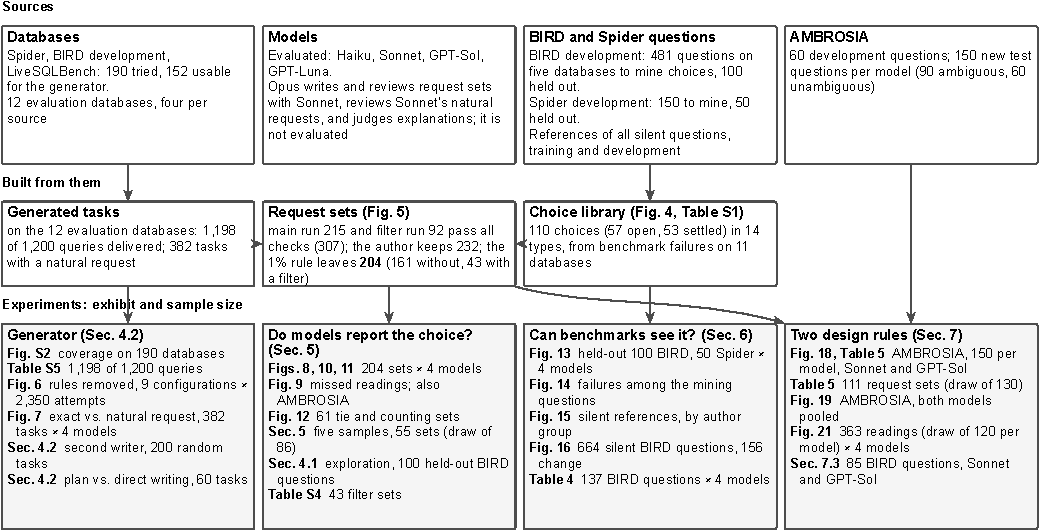
\includegraphics{diag_datamap.pdf}
\caption{Data and experiments: sources (top), data built from them (middle), and the experiments with their sample sizes (bottom). Arrows show what is built from what and what each experiment uses.}
\Description{Three rows of boxes. Sources: databases, models, BIRD and Spider questions, AMBROSIA. Built data: generated tasks, request sets, choice library. Experiments: generator, reporting, benchmarks, design rules, each with sample sizes.}
\label{fig:datamap}
\end{figure*}

\section{The Choices Are Common}
\label{sec:appendixlibrary}
\label{sec:catalogue}
The choices in the library are not quirks of one benchmark or one database. Table~\ref{tab:librarydetail} lists every type, how often BIRD and Spider references meet it, and how many request sets test it. Table~\ref{tab:catbreadth} shows on how many databases, and in which sources, each type occurs. Appendix~\ref{sec:typeexamples} gives examples of every type that a reader can check by hand.

\paragraph{The library.} Table~\ref{tab:librarydetail} gives the labels and counts in the fixed example library for every type. ``Open'' includes both unresolved and contested records. ``Settled'' denotes failure records the reviewers label as settled by the wording; this label is not the word-list check used for the defaults experiment. Failures that differ only in output format (51 with two accepted interpretations, 10 with one) are not choices of meaning and are not in the table. Possible reference errors (27) and unplaced cases (four) are also kept apart. For Table~\ref{tab:comparison}, AmbiQT's column and table ambiguity and AMBROSIA's vagueness map to \emph{which column}, AMBROSIA's scope to \emph{any vs.\ all}, and attachment to \emph{how conditions link}.

\begin{table}[t]
\caption{All choice types (Figure~\ref{fig:choices} of the paper shows the major ones). Library: choices of meaning in benchmark failures, open (the wording fits both interpretations) or settled (it selects one). References: BIRD and Spider questions silent on the choice, by the interpretation their reference SQL takes: the usual one, or the other with its share (\%), after the less common interpretations were reviewed; --: not readable from the SQL. Sets: the 204 accepted request sets, of the types whose other interpretation at least 1\% of silent references take. The library's value-representation type is split by its SQL edit: comparison strictness is a strict cutoff, any other edit value matching.}
\label{tab:librarydetail}
\centering\footnotesize\setlength{\tabcolsep}{2pt}
\begin{tabular*}{\columnwidth}{@{}l@{\hspace{3pt}}l@{\extracolsep{\fill}}rrrrr@{}}
\toprule
& & \multicolumn{2}{c}{Library} & \multicolumn{2}{c}{References} & \\
\cmidrule{3-4}\cmidrule{5-6}
Choice type & The choice & Open & Settled & Usual & Other (\%) & Sets\\
\midrule
Aggregation level & Rows or group averages? & 6 & 2 & 244 & 15 (5.8) & 61\\
Calculation & Which formula is meant? & 1 & 1 & 613 & 1 (0.2) & 0\\
Quantifier & ``Than any'': one or all? & 3 & 0 & 8 & 7 (46.7) & 0\\
Condition linkage & Conditions on one row? & 1 & 0 & 260 & 0 (0.0) & 0\\
Counting unit & Count rows or entities? & 7 & 27 & 2{,}521 & 237 (8.6) & 30\\
Missing values & Keep or skip missing? & 8 & 3 & 1{,}630 & 26 (1.6) & 29\\
Negation & Some non-match, or none? & 0 & 1 & 272 & 3 (1.1) & 1\\
Population scope & Keep unmatched rows? & 0 & 1 & 12{,}462 & 5 (0.0) & 0\\
Referent column & Which column is meant? & 19 & 6 & -- & -- & 0\\
Relationship role & Which link to follow? & 2 & 4 & 15 & 0 (0.0) & 0\\
Strict cutoff & Strict or inclusive? & 1 & 0 & 309 & 5 (1.6) & 42\\
Ties and selection & One tied row, or all? & 7 & 3 & 2{,}826 & 397 (12.3) & 41\\
Time scope & Period? Ends included? & 1 & 2 & 254 & 1 (0.4) & 0\\
Value matching & Exact or loose match? & 1 & 3 & 9{,}330 & 22 (0.2) & 0\\
\midrule
\multicolumn{2}{@{}l}{Total} & 57 & 53 & & & 204\\
\bottomrule
\end{tabular*}
\end{table}

\paragraph{How references are counted.} The References columns of Table~\ref{tab:librarydetail} read each reference query with an SQL parser and the schema's keys and column types, without a model, and count a question only when its wording has no cue for the choice. Ties, counting unit, missing values, population scope, ``between'' and value matching follow Section~\ref{sec:defaults} of the paper; calculation is a question that says percent, answered times 100 or as a fraction. \emph{Quantifier}: a question that says ``than any'', answered by comparing with every value (\sql{> MAX}, \sql{< MIN}, \sql{ALL}) or with at least one (\sql{> MIN}, \sql{< MAX}, \sql{ANY}). \emph{Negation}: a negated question answered with no matching record (\sql{NOT IN}, \sql{NOT EXISTS} or \sql{EXCEPT} over another table) or with some non-matching record (\sql{<>} on the many side of a join). \emph{Aggregation level}: an entity ranked by a numeric column on the many side of a join, by one row's value or by a sum or average per group. \emph{Condition linkage}: two or more conditions on different columns of the many side of a join, on one row or on separate rows (the table joined twice by the same key, or an \sql{INTERSECT}). \emph{Relationship role}: two tables that share a parent and are also connected by a link table, joined through the parent or through the link table. Which column a phrase means depends on the words, not the SQL, so the referent column has no count.

\paragraph{A lower bound.} Each rule reads one SQL form of its choice, so it detects only part of the choices mined from failures: applied to the 85 library records of the twelve types, the rules find the choice in 50, including all ties and quantifier records, 27 of 34 counting records and 4 of 6 relationship records, but none of the aggregation, time scope or value matching records, whose forms (grouping by a non-key attribute, an average used as a threshold) the rules do not read. The counts are therefore a lower bound on how often the choices arise.

\paragraph{Review of the less common interpretations.} Every reference that takes the less common interpretation was then read against fixed criteria (the SQL takes that interpretation, the wording leaves the choice open, and the other interpretation could change the answer), and every verdict is listed in the package for the authors' review. Of 1,259 such references, 540 are dropped, most often because the wording settles the choice (``list the students with the highest'', ``how many different''), the join cannot repeat the counted entity, or a \sql{LIKE} only escapes an apostrophe. Only this side was reviewed, so the shares in the table are conservative. The same drops apply to Section~\ref{sec:defaults} of the paper.

\paragraph{Breadth.} Table~\ref{tab:catbreadth} counts every library choice by the benchmark whose failure revealed it, and every accepted request set by the source of its database. The library reflects where failures were diagnosed: its choices come from eleven databases, and several types were found in one benchmark only. The request sets show that the major types are not tied to those databases. Each of the five types with request sets beyond a single one occurs on at least eight of the twelve databases, and in databases from Spider, BIRD and LiveSQLBench.

\begin{table}[t]
\caption{Top: every library choice (Table~\ref{tab:librarydetail}), by the benchmark whose failures revealed it. Bottom: every accepted request set, by the source of its database. DBs: distinct databases.}
\label{tab:catbreadth}
\centering\footnotesize
\setlength{\tabcolsep}{2pt}% generated by python -m specbridge.report.catalogue_tex; do not edit
\begin{tabular*}{\columnwidth}{@{}l@{\extracolsep{\fill}}rrrrrrr@{}}
\toprule
& \multicolumn{3}{c}{Library choices} & \multicolumn{4}{c}{Accepted request sets}\\
\cmidrule{2-4}\cmidrule{5-8}
Choice type & BIRD & Spider & DBs & Spider & BIRD & LiveSQL & DBs\\
\midrule
Aggregation level & 8 & -- & 4 & 20 & 16 & 25 & 11\\
Calculation & 2 & -- & 2 & -- & -- & -- & --\\
Condition linkage & 1 & -- & 1 & -- & -- & -- & --\\
Counting unit & 33 & 1 & 4 & 12 & 1 & 17 & 8\\
Missing values & 8 & 3 & 5 & 12 & 16 & 1 & 9\\
Negation & 1 & -- & 1 & 1 & -- & -- & 1\\
Population scope & 1 & -- & 1 & -- & -- & -- & --\\
Quantifier & -- & 3 & 1 & -- & -- & -- & --\\
Referent column & 22 & 3 & 4 & -- & -- & -- & --\\
Relationship role & 5 & 1 & 2 & -- & -- & -- & --\\
Strict cutoff & 1 & -- & 1 & 17 & 16 & 9 & 10\\
Ties and selection & 8 & 2 & 6 & 9 & 12 & 20 & 11\\
Time scope & 3 & -- & 2 & -- & -- & -- & --\\
Value matching & 3 & 1 & 3 & -- & -- & -- & --\\
\midrule
Total & 96 & 14 & 11 & 71 & 61 & 72 & 12\\
\bottomrule
\end{tabular*}

\end{table}

\paragraph{Request sets.} Table~\ref{tab:librarydetail} counts the 204 accepted request sets by type, 43 of them with a choice in a filter (Appendix~\ref{sec:filtersets}). Over the 215 sets whose choice a model proposes, aggregation level contributes 63, ties 44, missing values 40, counting unit 35, calculation 15, relationship role nine, and time scope two. The remaining seven belong to the six additional labels: running-total interpretation (two), active-status filtering, comparison baseline, baseline population, baseline definition, and row-count versus quantity measurement (one each). These counts reflect the generation and selection procedure.

\section{Calculation Choices with Real Consequences}
\label{sec:cases}
Table~\ref{tab:cases} surveys documented cases, across six domains, in which one open or mistaken choice of the kind our library records changed a consequential number or decision. None is a text-to-SQL failure. Each entry was checked against the original paper or official report; we left out cases whose primary source we could not reach, such as a bank's value-at-risk spreadsheet and a classic study of graduate admissions.

\begin{table*}[t]
\caption{Documented cases where one calculation choice changed a consequential number or decision, by domain, with the closest choice type in our library.}
\label{tab:cases}
\centering\footnotesize\setlength{\tabcolsep}{4pt}\renewcommand{\arraystretch}{1.1}
\begin{tabularx}{\textwidth}{@{}>{\raggedright\arraybackslash}p{2.2cm}>{\raggedright\arraybackslash}p{3.3cm}>{\raggedright\arraybackslash}X>{\raggedright\arraybackslash}p{2.6cm}@{}}
\toprule
Domain & Case & Choice and consequence & Library type\\
\midrule
Economics and policy & Public debt and growth~\cite{herndon2014debt} & Growth was averaged within each country before averaging across countries, so one year of New Zealand data weighed as much as decades of another country. With corrected data and weighting, high-debt countries grew 2.2\% a year, not $-0.1\%$. & aggregation level\\
\specialrule{0.2pt}{1.5pt}{1.5pt}
Health care & Risk algorithm for extra care~\cite{obermeyer2019bias} & ``Need'' was computed as health-care cost. The algorithm looked accurate by standard measures, yet fixing the proxy would raise the share of Black patients receiving extra help from 17.7\% to 46.5\%. & which column a phrase means\\
\specialrule{0.2pt}{1.5pt}{1.5pt}
Health care & Hospital mortality rates~\cite{shahian2010mortality} & Four methods, given the same 2.5 million discharges, included 28--95\% of them. 12 of 28 hospitals with higher-than-expected mortality by one method had lower-than-expected mortality by another. & population scope\\
\specialrule{0.2pt}{1.5pt}{1.5pt}
Public health & 1995 UK contraceptive pill warning~\cite{furedi1999pill} & A warning of higher thrombosis risk for two pill types was followed by pill use among under-16s falling from 40\% to 27\%, and by estimated NHS costs of \pounds 21 million for maternity care and \pounds 46 million for abortions. The author concludes that risk should be more carefully presented. & how a quantity is stated (not in our library)\\
\specialrule{0.2pt}{1.5pt}{1.5pt}
Social science & Referees and skin tone~\cite{silberzahn2018many} & 29 teams analysed the same data. Their odds ratios ranged from 0.89 to 2.93; 20 teams found a significant effect and 9 did not, using 21 combinations of covariates. & several analysis choices\\
\specialrule{0.2pt}{1.5pt}{1.5pt}
Science & Brain imaging~\cite{botviniknezer2020variability} & 70 teams analysed one dataset to test the same 9 hypotheses. No two chose the same workflow, and the results of the hypothesis tests varied substantially. & several analysis choices\\
\specialrule{0.2pt}{1.5pt}{1.5pt}
Science & Gene names in spreadsheets~\cite{ziemann2016gene} & Spreadsheet software converts gene names to dates and numbers by default; about one fifth of papers with supplementary gene lists in spreadsheets contain such conversions. & value representation\\
\specialrule{0.2pt}{1.5pt}{1.5pt}
Engineering & Mars Climate Orbiter~\cite{nasa1999mco} & Thruster data in English units were used where the trajectory software expected metric units; the spacecraft was lost. & value representation\\
\specialrule{0.2pt}{1.5pt}{1.5pt}
Engineering & Ariane 5 flight 501~\cite{lions1996ariane} & A 64-bit floating-point value was converted to a 16-bit signed integer that could not hold it; the launcher broke up about 40 seconds after lift-off. & value representation\\
\bottomrule
\end{tabularx}
\end{table*}

\section{Request Sets with Filter Conditions}
\label{sec:filtersets}
The filter sets of Section~\ref{sec:filters} of the paper come from one optional rule of the generator. It adds a single condition to the first stage of a query, on the rows of that stage's table, and builds the second interpretation at the same time. The five forms are: a date range, inclusive (\sql{>=} and \sql{<=}) or exclusive (\sql{>} and \sql{<}), with ends at the 30th and 70th percentile of a date column; a cutoff at a frequent value of a measure, \sql{>= v} or \sql{> v}; ``without'' a category, no record of the entity has it (\sql{NOT IN}) or some record lacks it (\sql{IN} with \sql{<>}); two categories, on one record or on any records of the entity; and a per-entity count, over entities with matching rows (inner join) or over all entities (outer join, zero counts kept). The generator prefers forms it has used less often. The seed is 20261016; 161 of 180 requested queries are delivered, 121 of them have interpretations with different answers, and 92 request sets pass all checks.

\paragraph{Results.} Table~\ref{tab:filtersets} gives the results per model on the 43 accepted filter sets. What models raise follows the wording of the open request. Forty of the 42 cutoff requests give a value ``as the cutoff'' or ``threshold,'' with no comparison word, and the other two say ``upwards of''; models return both the strict and the inclusive interpretation in 115 of the 159 cases where they compute both. The settled request is never called open. GPT-Luna returns both interpretations least often, as on the other sets.

\begin{table}[t]
\caption{Filter request sets (43 accepted), per model: both specific requests right (with exploration); among those, open requests answered with both interpretations; open requests that name the choice (Opus judge); specific requests right (single call); missed interpretations the model computes when asked, of all missed.}
\label{tab:filtersets}
\centering\footnotesize\setlength{\tabcolsep}{4pt}
\begin{tabular}{@{}lrrrrr@{}}
\toprule
Model & Both right & Both returned & Named & Right & Missed, computable\\
\midrule
Haiku & 42 & 33 & 40 & 40 & 9 / 10\\
Sonnet & 41 & 36 & 38 & 42 & 5 / 6\\
GPT-Sol & 42 & 32 & 35 & 40 & 10 / 10\\
GPT-Luna & 38 & 14 & 25 & 41 & 24 / 29\\
\bottomrule
\end{tabular}
\end{table}

\paragraph{Rejected sets.} The authors reject all 17 date-range sets. Every date-range request says ``between,'' which SQL's \sql{BETWEEN} includes, and 254 of the 255 BIRD and Spider references whose question says ``between'' with no other cue include both ends. Among the BIRD and Spider references whose question says ``between'' with no other cue, the one that excludes the ends is a Spider reference that applies strict bounds to the start and end columns of a staff role. A BIRD reference whose evidence says \sql{BETWEEN 121 AND 130} but whose query excludes both ends is not counted, since its evidence settles the ends. Four further references use strict bounds moved one step out, or a negated range, and select the inclusive range. Of the 49 rejected sets, 17 are the date ranges, 15 are cutoffs whose wording (``passes'', ``clears'', ``on the high side of'') already makes the comparison strict, five are ``without'' requests that already mean no such record, and one is a per-entity average whose request restricts the population. The other 11 test per-entity counts with or without unmatched entities (eight) and conditions on one or any records (three), choices whose other interpretation real references almost never take (Figure~\ref{fig:choices} of the paper).

\section{Query Generation Details}
\label{sec:querydetails}
Algorithm~\ref{alg:families} lists the construction of a request set, Figure~\ref{fig:ablation} shows what each construction rule contributes, and Figure~\ref{fig:specification} compares the exact description with the natural request. Figure~\ref{fig:coverage} shows, for each feature, the share of 152 databases whose schema allows it and the share where a generated query with it was accepted by both model reviewers; and Table~\ref{tab:construction} the queries delivered on the 12 evaluation databases.

\textbf{Formal statement.} Let $\mathcal L(K_D)$ be the queries that the catalogue $K_D$ of database $D$ and the type rules allow, $\delta(p)$ a query's arithmetic and step depth, and $O(p)$ its operations. For target depths $d$ and required operations $R$ the generator samples from
\begin{equation}
\mathcal P(D,d,R)=\{p\in\mathcal L(K_D):\delta(p)=d,\ R\subseteq O(p),\ I_D(p)=1\},
\end{equation}
where $I_D(p)=1$ means that all data checks pass. It keeps a partial query $z$ only if some completion can still reach the target,
\begin{equation}
\operatorname{can}(z,d,R)=\mathbf 1\{\exists(d,U)\in\operatorname{Reach}(z):R\subseteq U\},
\label{eq:reach}
\end{equation}
where $\operatorname{Reach}(z)$ lists the depths and operation sets still possible. The look-ahead is exact for the rules, and no query is drawn twice. For a request set $F$ with specific requests $q_A,q_B$ and open request $q_\circ$, let $H^{(r)}_{ij}=1$ when reviewer $r$ accepts request $i$ for interpretation $j$, $f_r=1$ when $r$ finds no changed or missing requirement, and $c(F)=1$ when all code checks pass. The set is kept when
\begin{equation}
\begin{split}
\operatorname{keep}(F)=c(F)&\land\bigwedge_r\left[f_r\land H^{(r)}_{\{A,B\},\{A,B\}}=I_2\right]\\
&\land\bigvee_r\left[H^{(r)}_{\circ A}\land H^{(r)}_{\circ B}\right].
\end{split}
\end{equation}

\begin{algorithm}[t]
\caption{Build a request set around one calculation choice}
\label{alg:families}
\begin{algorithmic}[1]
\Require Databases $D$, target depths $d$, required operations $R$
\Ensure Accepted request sets and reasons for rejected sets
\For{each requested task}
\State Sample $p_A\in\mathcal P(D,d,R)$ with the look-ahead of Eq.~\eqref{eq:reach}
\State If no query is delivered, record the shortfall and continue
\State Describe $p_A$; write and check its request
\State Propose edits $p_A\rightarrow p_B$ that express a different choice
\State Execute and describe both queries; require different answers
\State Repair failed proposals once; review both interpretations
\EndFor
\State Select one choice per task at most, balancing types and databases
\For{each selected choice}
\State List what stays fixed and what changes
\State Write requests specifying A, specifying B, and leaving it open
\State Check requirements and all six request--interpretation pairs
\State Revise a failing set once and recheck
\State Keep $F$ if $\operatorname{keep}(F)$; otherwise record the reason
\EndFor
\end{algorithmic}
\end{algorithm}

\begin{figure}[t]
\centering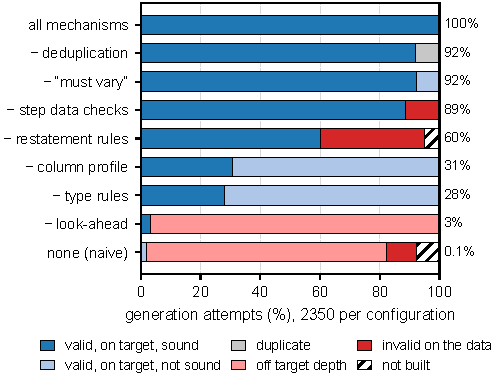
\includegraphics[width=\columnwidth]{col_ablation.pdf}
\caption{Generation outcomes with each construction rule removed (2,350 attempts). The labels give the share valid, on target and sound.}
\Description{Stacked bars of generation outcomes for nine configurations.}
\label{fig:ablation}
\end{figure}
\begin{figure}[t]
\centering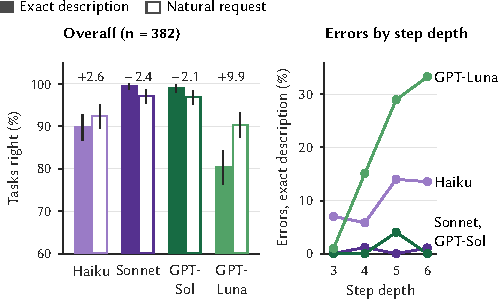
\includegraphics[width=\columnwidth]{col_specification.pdf}
\caption{Exact description versus natural request on 382 generated tasks. Left: accuracy; numbers give the difference in points. Right: errors from the exact description by step depth.}
\Description{Bars for four models under two request forms, and lines of error rate by step depth.}
\label{fig:specification}
\end{figure}
\begin{figure}[t]
\centering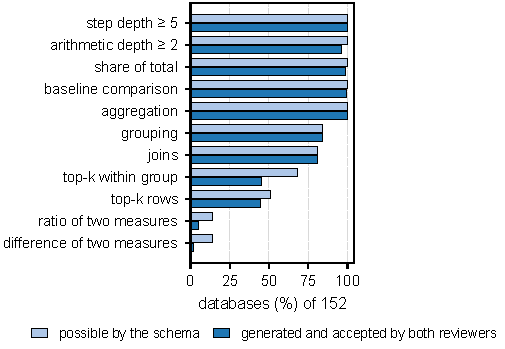
\includegraphics[width=\columnwidth]{col_coverage.pdf}
\caption{Features the generator can build, as a share of 152 databases: possible by the schema, and generated and accepted.}
\Description{Paired horizontal bars for eleven features: possible by the schema versus generated and accepted.}
\label{fig:coverage}
\end{figure}
\begin{table}[t]
\caption{Program construction on 12 databases, with no model calls after catalogue preparation. Every delivered SQL is distinct, has the requested depth, and passes both integrity checks.}
\label{tab:construction}
\centering\small
\renewcommand{\arraystretch}{1.12}
\begin{tabular}{@{}lrrrr@{}}
\toprule
Source & DBs & Delivered & Constructions & Seconds\\
\midrule
Spider & 4 & 398/400 & 289 & 127\\
BIRD & 4 & 400/400 & 270 & 274\\
LiveSQLBench & 4 & 400/400 & 309 & 37\\
\midrule
Total & 12 & 1198/1200 & 868 & 437\\
\bottomrule
\end{tabular}
\par\smallskip\footnotesize Source-level times are rounded individually; the total is rounded from the unrounded sum. Separate task review delivers 384/400 tasks, and language generation supplies 382/384 requests.
\end{table}
\section{Seeds, Versions and Selection Rules}
\label{sec:furtherdetails}
\paragraph{Seeds, versions and reruns.}
The grammar is \texttt{compose-v3.4}. Task requests, Spider splitting, request set selection, explanation allocation, and bootstrap resampling use seed 20261003; BIRD holdout selection uses 20261001; the paired wording comparison uses 20261004. Coverage uses seed 1 and depth-control runs seeds 1--3. Python was 3.11.5 and SQLite 3.41.2. During the experiments, the Claude command-line client changed from 2.1.287 to 2.1.289 and the Codex client from 0.147 to 0.160. Temporary usage-limit outputs were removed and retried rather than treated as SQL answers. A final query that failed under concurrent execution was rerun alone: ten such answers then matched their reference (nine GPT-Luna, one GPT-Sol). Token counts are unavailable for the explanation runs, so latency is reported instead of cost.

\paragraph{Rewrite comparison.}
The comparison of the original specific request (a) with the other texts was fixed before the run. The comparisons with the edited request (c) were added after an interim look at half of the interpretations.

\paragraph{Response selection.}
The explanation examples are the first saved responses displaying each tested pattern in file order. The worked aggregation example uses the smallest case-identifier hash among eligible request sets. Library examples use the first eligible record per type at high confidence, or medium confidence if none is high, with fixed benchmark and task ordering. Generated examples outside library labels enumerate retained cases before selecting the four shown in the main text. These selection rules support traceability; illustrative examples are not frequency estimates.

\section{Examples of Each Choice Type}
\label{sec:typeexamples}
Tables~\ref{tab:catlibrary} and~\ref{tab:catsets} show examples of each type, selected by a fixed rule rather than by hand. Library choices are taken from different databases, open choices before choices the wording settles, one from each benchmark when the type has both, shortest question first. Request sets are taken from different databases, one per source in turn, shortest open request first. Each example's question or request is given as the model received it. Answers says how the two reference queries' results differ on the database. Models gives each model's answer to the open request in one call with explanation, in the order Haiku, Sonnet, GPT-Sol, GPT-Luna: B, both interpretations returned; N, one interpretation, with the choice named; S, one interpretation given silently, although the model computes each interpretation when asked; a dash, one interpretation, and the model does not compute both. The package holds every choice and every set, with its SQL.

\onecolumn
{\scriptsize\setlength{\tabcolsep}{3pt}\renewcommand{\arraystretch}{1.05}
% generated by python -m specbridge.report.catalogue_tex; do not edit
\begin{xltabular}{\textwidth}{@{}>{\raggedright\arraybackslash}p{2.3cm}>{\hsize=1.15\hsize\raggedright\arraybackslash}X>{\hsize=0.85\hsize\raggedright\arraybackslash}X>{\raggedright\arraybackslash}p{1.2cm}@{}}
\caption{Selected library choices, up to 3 per type.}\label{tab:catlibrary}\\
\toprule
Source & Question & The choice & Wording\\
\midrule
\endfirsthead
\toprule
Source & Question & The choice & Wording\\
\midrule
\endhead
\bottomrule
\endfoot
\multicolumn{4}{@{}l}{\textbf{Aggregation level} (3 of 8 shown)}\\[1pt]
BIRD, \texttt{california\_\allowbreak{}schools} & Which active district has the highest average score in Reading? & Whether to rank districts by one school's AvgScrRead value or by the average of AvgScrRead across each district's schools & open\\[2pt]
BIRD, \texttt{financial} & Who are the account holder identification numbers whose who have transactions on the credit card with the amount is less than the average, in 1998? Evidence: Operation = 'VYBER KARTOU' refers to credit card withdrawal & Which transactions the 'average' amount threshold is computed over & open\\[2pt]
BIRD, \texttt{thrombosis\_\allowbreak{}prediction} & For all patient born in 1982, state if their albumin is within normal range. Evidence: Year(Birthday) = '1982'; albumin is within normal range refers to ALB between 3.5 and 5.5 & Whether the normal/abnormal status is given once per laboratory record or once per patient born in 1982, since each patient can have many Laboratory rows & open\\[2pt]
\midrule
\multicolumn{4}{@{}l}{\textbf{Calculation} (2 of 2 shown)}\\[1pt]
BIRD, \texttt{financial} & Provide the IDs and age of the client with high level credit card, which is eligible for loans. Evidence: the credit card is high-level refers to card.type = 'gold'; eligible for loans refers to disp.type = 'OWNER' & How to compute the client's age from birth\_date: subtract the birth year from the current year, or count completed years of life. & open\\[2pt]
BIRD, \texttt{thrombosis\_\allowbreak{}prediction} & For all patients who are older than 55 years old, what is the percentage of female who has abnormal prothrombin time (PT)? Evidence: older than 55 years old = SUBTRACT(year(current\_timestamp), year(Birthday)) \textgreater{} 55; abnormal prothrombin time (PT) refers to PT \textgreater{} = 14; percentage = DIVIDE(SUM(PT \textgreater{} = 14 AND SEX = 'F'), SUM(PT \textgreater{} = 14)) * 100; female refers to sex = 'F'; & Which population the percentage is taken over (the denominator) & settles it\\[2pt]
\midrule
\multicolumn{4}{@{}l}{\textbf{Condition linkage} (1 of 1 shown)}\\[1pt]
BIRD, \texttt{toxicology} & Calculate the percentage of carcinogenic molecules with triple bonded Hidrogen atoms. Evidence: hydrogen refers to element = 'h'; label = '+' mean molecules are carcinogenic; triple bond refers to bond\_type = '\#'; percentage = DIVIDE(SUM(label = '+'), COUNT(molecule\_id)) * 100.0 where element = 'h' AND bond\_type = '\#'; & How a hydrogen atom is tied to a triple bond: either the hydrogen is one of the two atoms in the '\#' bond (linked through \texttt{connected}), or the hydrogen and some '\#' bond just appear in the same molecule (linked only through molecule\_id). & open\\[2pt]
\midrule
\multicolumn{4}{@{}l}{\textbf{Counting unit} (3 of 34 shown)}\\[1pt]
BIRD, \texttt{thrombosis\_\allowbreak{}prediction} & What is the average age of the male patient with high cholesterol? Evidence: average age = DIVIDE(SUM(SUBTRACT(YEAR(NOW()), YEAR(birthday))), COUNT(ID)); male patient refers to sex = 'M'; high cholesterol refers to \texttt{T-CHO} \textgreater{} = 250; & Whether the average is taken once per patient or once per matching lab record, since a patient can have several Laboratory rows with T-CHO \textgreater{}= 250 & open\\[2pt]
BIRD, \texttt{toxicology} & What is the least common element of all carcinogenic molecules? Evidence: label = '+' mean molecules are carcinogenic & What unit 'least common' is counted in: the number of carcinogenic molecules that contain the element, or the number of atoms of that element across all carcinogenic molecules & open\\[2pt]
Spider, \texttt{student\_\allowbreak{}transcripts\_\allowbreak{}tracking} & How many different degrees are offered? & What counts as one degree: a distinct degree name (degree\_summary\_name) or each degree program row in Degree\_Programs & open\\[2pt]
\midrule
\multicolumn{4}{@{}l}{\textbf{Missing values} (3 of 11 shown)}\\[1pt]
BIRD, \texttt{california\_\allowbreak{}schools} & What is the phone number of the school that has the highest average score in Math? & How to handle the top AvgScrMath row in satscores when it has no matching record in schools: drop it and take the best-scoring school that does have a record, or keep it as the answer even though its phone is missing. & open\\[2pt]
Spider, \texttt{cre\_\allowbreak{}Doc\_\allowbreak{}Template\_\allowbreak{}Mgt} & Show all template ids and number of documents using each template. & Whether templates that no document uses should appear in the output with a count of 0, or only templates that at least one document uses should be listed & open\\[2pt]
Spider, \texttt{network\_\allowbreak{}1} & Show the student IDs and numbers of friends corresponding to each. & Whether students who have no rows in Friend should be listed with a count of 0, or left out. & open\\[2pt]
\midrule
\multicolumn{4}{@{}l}{\textbf{Negation} (1 of 1 shown)}\\[1pt]
BIRD, \texttt{toxicology} & What percentage of carcinogenic-type molecules does not contain fluorine? Evidence: label = '+' mean molecules are carcinogenic; contain fluorine refers to element = 'f'; percentage = DIVIDE(SUM(element = 'f') * 100, COUNT(molecule\_id)) where label = '+'; Should consider the distinct atoms when counting; & What it means for a carcinogenic molecule to 'not contain fluorine': the molecule has at least one atom that is not fluorine, or the molecule has no fluorine atom at all. & settles it\\[2pt]
\midrule
\multicolumn{4}{@{}l}{\textbf{Population scope} (1 of 1 shown)}\\[1pt]
BIRD, \texttt{thrombosis\_\allowbreak{}prediction} & How many patients with an Ig G higher than normal? Evidence: Ig G higher than normal refers to IGG \textgreater{}= 2000; Should consider DISTINCT in the final result; & Whether the patient count only includes patients who also have records in the Examination table (because of the inner join to Examination), or every patient with any lab IgG result of at least 2000 & settles it\\[2pt]
\midrule
\multicolumn{4}{@{}l}{\textbf{Quantifier} (1 of 3 shown)}\\[1pt]
Spider, \texttt{world\_\allowbreak{}1} & What are the countries that have greater surface area than any country in Europe? & Whether 'greater than any country in Europe' means larger than at least one European country (compare to the smallest European area) or larger than every European country (compare to the largest European area) & open\\[2pt]
\midrule
\multicolumn{4}{@{}l}{\textbf{Referent column} (3 of 25 shown)}\\[1pt]
BIRD, \texttt{california\_\allowbreak{}schools} & Please specify all of the schools and their related mailing zip codes that are under Avetik Atoian's administration. & Which administrator slots count as being 'under Avetik Atoian's administration': only the primary administrator columns (AdmFName1/AdmLName1), or any of the three administrator slots. & open\\[2pt]
BIRD, \texttt{financial} & What year was account owner number 130 born? & Which ID the number 130 in 'account owner number 130' refers to: the account ID or the client ID & open\\[2pt]
Spider, \texttt{car\_\allowbreak{}1} & What are the makers and models? & Which column supplies 'makers': the integer foreign key model\_list.Maker, or the maker name car\_makers.Maker reached by joining on that key & open\\[2pt]
\midrule
\multicolumn{4}{@{}l}{\textbf{Relationship role} (2 of 6 shown)}\\[1pt]
BIRD, \texttt{toxicology} & Which molecule consisted of Sulphur atom with double bond? Evidence: sulphur refers to element - 's'; double bond refers to bond\_type = ' = '; & Does the sulfur atom itself have to be part of the double bond, or is it enough that the molecule has both a sulfur atom and a double bond somewhere? & open\\[2pt]
Spider, \texttt{network\_\allowbreak{}1} & What is the lowest grade of students who do not have any friends? & Whether a student who appears in Friend only as friend\_id (someone else lists them as a friend) counts as having a friend & open\\[2pt]
\midrule
\multicolumn{4}{@{}l}{\textbf{Strict cutoff} (1 of 1 shown)}\\[1pt]
BIRD, \texttt{thrombosis\_\allowbreak{}prediction} & Provide the ID and age of patient with lactate dehydrogenase (LDH) between 100-300 index above the normal range. Evidence: age refers to SUBTRACT(year(current\_timestamp), year(Birthday)); lactate dehydrogenase (LDH) between 100-300 index above the normal range refers to LDH between 600 and 800; & Whether the LDH range endpoints 600 and 800 are included (strict vs. inclusive bounds) & open\\[2pt]
\midrule
\multicolumn{4}{@{}l}{\textbf{Ties and selection} (3 of 10 shown)}\\[1pt]
BIRD, \texttt{superhero} & Give the hero ID of superhero with the lowest attribute value. Evidence: lowest attribute value refers to MIN(attribute\_value); & How to handle ties at the minimum attribute\_value: return every tied hero, or return just one hero as the singular 'the hero ID' suggests. & open\\[2pt]
BIRD, \texttt{thrombosis\_\allowbreak{}prediction} & For the patient who has the highest Ig A within the normal range, what is his or her diagnosis? Evidence: highest Ig A within the normal range refers to MAX(IGA BETWEEN 80 AND 500); & How to handle several lab records tied at the maximum in-range IgA value (IGA = 500): return one row or every tied patient's diagnosis. & open\\[2pt]
Spider, \texttt{world\_\allowbreak{}1} & Give the name of the nation that uses the greatest amount of languages. & Several countries tie for the most languages (12). The question does not say which of them to return, so the answer depends on how the tie is broken. & settles it\\[2pt]
\midrule
\multicolumn{4}{@{}l}{\textbf{Time scope} (2 of 3 shown)}\\[1pt]
BIRD, \texttt{financial} & For the client who applied the biggest loan, what was his/her first amount of transaction after opened the account? & Whether a transaction on the account-opening date counts as 'after opened the account' (inclusive vs. strictly later boundary) & open\\[2pt]
BIRD, \texttt{thrombosis\_\allowbreak{}prediction} & For all patients with normal uric acid (UA), what is the average UA index based on their latest laboratory examination result? Evidence: uric acid (UA) with normal range refers to UA \textless{} 8.0 and SEX = 'M' or UA \textless{} 6.5 and SEX = 'F'; average UA index refers to AVG(UA) & Which date counts as the 'latest laboratory examination': the single latest date in the whole Laboratory table, or each patient's own latest test date & settles it\\[2pt]
\midrule
\multicolumn{4}{@{}l}{\textbf{Value matching} (3 of 4 shown)}\\[1pt]
BIRD, \texttt{financial} & How much, in total, did client number 617 pay for all of the transactions in 1998? & Which 1998 transactions count as the client having 'paid': every transaction on the client's accounts, or only outgoing ones (debits). & open\\[2pt]
BIRD, \texttt{thrombosis\_\allowbreak{}prediction} & Please list the disease names of the patients that have a proteinuria level higher than normal. Evidence: disease names refers to Diagnosis; proteinuria level higher than normal refers to \texttt{U-PRO} \textgreater{} = 30; & Whether the threshold \texttt{U-PRO} \textgreater{}= 30 compares the TEXT column \texttt{U-PRO} as text (string order) or as numbers & settles it\\[2pt]
Spider, \texttt{car\_\allowbreak{}1} & Which model saves the most gasoline? That is to say, have the maximum miles per gallon. & Whether the TEXT-typed MPG column is ranked by its stored string value or by its numeric value when picking the maximum & settles it\\[2pt]
\end{xltabular}

% generated by python -m specbridge.report.catalogue_tex; do not edit
\begin{xltabular}{\textwidth}{@{}>{\raggedright\arraybackslash}p{1.5cm}>{\hsize=1.45\hsize\raggedright\arraybackslash}X>{\hsize=0.95\hsize\raggedright\arraybackslash}X>{\raggedright\arraybackslash}p{1.9cm}>{\hsize=0.6\hsize\raggedright\arraybackslash}X>{\centering\arraybackslash}p{1.05cm}@{}}
\caption{Every accepted request set (204, 43 of them with a filter condition), by choice type. Open request: the text the models were given (each set also has one specific request per reading). Results: how the two reference answers differ on the database. Review: the author's reason for accepting the set. Models (Haiku, Sonnet, GPT-Sol, GPT-Luna), for the open request in one call with explanation: B both readings returned; N one reading, the choice named; S one reading, silent, although the model computes both when asked; -- one reading, and the model does not compute both. Full sets with SQL, schema and grading: \texttt{benchmark/request\_sets.jsonl}, by set id.}
\label{tab:catsets}\\
\toprule
Set & Open request & Readings & Results & Review & Models\\
\midrule
\endfirsthead
\toprule
Set & Open request & Readings & Results & Review & Models\\
\midrule
\endhead
\bottomrule
\endfoot
\multicolumn{6}{@{}l}{\textbf{Aggregation level}}\\[1pt]
\texttt{7c4a89c45b}\newline\texttt{alien} & Which RFI statuses (\texttt{rfistat}) have an above-average modulation index (\texttt{modindex})? Ignore missing index values, and treat signals with no status as their own group. For each such status, show the status, its average modulation index, how far above average it is, and how it differs from the mean of the qualifying statuses' averages. Leave all values unrounded. & \textbf{A:} A status counts as above average if its mean modulation index exceeds the simple mean of the per-status means.\newline \textbf{B:} A status counts as above average if its mean modulation index exceeds the mean modulation index over all signals. & A: 2 rows, B: 2 rows; first row differs; largest value change: 0.003134 (A) vs 0.00293 (B), 6.5\% & The comparison baseline does not specify equal weighting of group averages versus pooling the underlying records. Both are plausible; pooled records give more weight to groups with more observations. & \texttt{-\,B\,B\,S}\\[2pt]
\texttt{9bb5ac76bd}\newline\texttt{alien} & Linking signals to their telescopes and observatories (signals that don't match are dropped), find the average modulation index and average phase shift for each telescope and weather profile (\texttt{weathprofile}). Keep the telescope/weather groups whose modulation index is above the overall average modulation index. Then, per weather profile, show the average modulation index and average phase shift of those groups, and how far above the overall average they are on average. Don't round anything. & \textbf{A:} The baseline is the average of the group-level averages, with every telescope/weather group counting equally.\newline \textbf{B:} The baseline is the average modulation index over all linked signals, with every signal counting equally. & A: 3 rows, B: 3 rows; first row differs; largest value change: 185.7 (A) vs 184.6 (B), 0.59\% & The comparison baseline does not specify equal weighting of group averages versus pooling the underlying records. Both are plausible; pooled records give more weight to groups with more observations. & \texttt{B\,B\,B\,-}\\[2pt]
\texttt{cde68b2348}\newline\texttt{alien} & For observatory stations whose average telescope bandwidth usage (\texttt{bandusagepct}) is above average, what is their mean bandwidth usage, and how far above average are they on average? Ignore missing usage values, and give both figures unrounded in a single row. & \textbf{A:} Compare each station's average bandwidth usage with the unweighted mean of the station averages.\newline \textbf{B:} Compare each station's average bandwidth usage with the mean bandwidth usage over all individual telescopes. & A: 1 row, B: 1 row; first row differs; largest value change: 24.9 (A) vs 25.03 (B), 0.52\% & The comparison baseline does not specify equal weighting of group averages versus pooling the underlying records. Both are plausible; pooled records give more weight to groups with more observations. & \texttt{S\,B\,B\,N}\\[2pt]
\texttt{d31fb48995}\newline\texttt{alien} & For each telescope in the signals table (\texttt{telescref}), work out its average pulse rate (\texttt{pulsepersec}), ignoring missing values, and keep the telescopes whose average is above the overall average pulse rate. Among those, keep only the ones whose average is also above the average of the kept telescopes' averages. In one row, give these final telescopes' mean average pulse rate, how far on average they sit above the overall average, and how far on average they sit above that second average. Don't round anything. & \textbf{A:} The overall baseline pulse rate is the average of the per-telescope average pulse rates, with each telescope weighted equally.\newline \textbf{B:} The overall baseline pulse rate is the average pulse rate over all signal records, with each signal weighted equally. & A: 1 row, B: 1 row; first row differs; largest value change: 1.213 (A) vs 1.208 (B), 0.44\% & The comparison baseline does not specify equal weighting of group averages versus pooling the underlying records. Both are plausible; pooled records give more weight to groups with more observations. & \texttt{S\,B\,S\,S}\\[2pt]
\texttt{e7b2c8e815}\newline\texttt{alien} & Which observatory stations (\texttt{observstation}) have an average telescope bandwidth usage (\texttt{bandusagepct}) above the overall average bandwidth usage? Ignore missing values. For each one, show the station, its average bandwidth usage, and how much it exceeds the overall average. Return the top 10 by that margin, largest first, without rounding. & \textbf{A:} Each station's average bandwidth usage is compared against the mean of the station averages, with every station weighted equally.\newline \textbf{B:} Each station's average bandwidth usage is compared against the mean bandwidth usage over all individual telescopes. & A: 10 rows, B: 10 rows; first row differs; largest value change: 49.42 (A) vs 49.54 (B), 0.26\% & The comparison baseline does not specify equal weighting of group averages versus pooling the underlying records. Both are plausible; pooled records give more weight to groups with more observations. & \texttt{S\,B\,S\,S}\\[2pt]
\texttt{1a73aa1ae0}\newline\texttt{archeology} & For environment records that match a site, show each site access status (\texttt{entrystat}) with its average ambient temperature (\texttt{ambictemp}) and average image count (\texttt{imgcount}). Also show how far that image-count average sits above or below the average image count overall (status average minus overall). Ignore missing values and don't round. & \textbf{A:} Compare each status's average image count with the mean of the status-level averages.\newline \textbf{B:} Compare each status's average image count with the average image count over all matched environment records. & A: 3 rows, B: 3 rows; first row differs; largest value change: -11.54 (A) vs -10.94 (B), 5.2\% & Overall can refer to matched records or the displayed status groups. B is more natural; A requires equal status weighting. & \texttt{S\,S\,S\,S}\\[2pt]
\texttt{1d3fc42a2c}\newline\texttt{archeology} & Match each spatial record (\texttt{scanspatial}) to the project whose \texttt{arcregistry} equals its \texttt{arcref}, and drop records with no matching project. What is each project's bounding-box X-to-Z ratio (\texttt{boxx} to \texttt{boxz}), ignoring missing values? Which 10 projects beat the simple average ratio of the projects in their own funding source (\texttt{projects.\allowbreak{}fundflux}) by the widest margin? Show the project ID, funding source, ratio and margin, sorted by margin from largest to smallest (missing last), with no rounding. & \textbf{A:} A project's ratio is the mean of its per-record boxx/boxz ratios.\newline \textbf{B:} A project's ratio is its total boxx divided by its total boxz. & A: 10 rows, B: 10 rows; first row differs; largest value change: 27.87 (A) vs 27.96 (B), 0.29\% & The within-group ratio is not operationally defined: averaging record-level ratios and dividing aggregated numerator by aggregated denominator are both plausible. They weight records differently; missing-value pairing also needs a policy. & \texttt{N\,B\,N\,N}\\[2pt]
\texttt{284b059491}\newline\texttt{archeology} & In the feature scan data, which 10 site artifact counts (\texttt{articount}, identified by site code \texttt{zoneref}) stand furthest above the average in their share of all artifacts? Each count's share is that count divided by the overall artifact total across all of \texttt{scanfeatures} (return nothing if the overall total is missing), and the average share is the mean of those shares (again return nothing if that average is missing). For each, give the site code, the artifact count, its share, and its share minus the average share. Ignore missing counts, and sort from the highest difference down with missing values last. & \textbf{A:} Total the artifact counts per site, then compute and rank each site's share against the average site share.\newline \textbf{B:} Treat each feature record separately, then compute and rank each record's share against the average record share. & A: 10 rows, B: 10 rows; first row differs; 18 row keys in only one answer; largest value change: 0.002942 (A) vs 0.001054 (B), 64\% & Site artifact counts suggests site totals, while each count and the named field suggest individual records. The intended row grain is unclear. & \texttt{B\,B\,-\,-}\\[2pt]
\texttt{30b46b4254}\newline\texttt{archeology} & Looking only at scans that match a site, what's the GB-per-minute rate of file size (\texttt{gbsize}) to scan duration (\texttt{spanmin}) for each site risk evaluation status (\texttt{riskeval}), treating scans at sites with no recorded status as a group of their own? Use the plain average of those group rates as a benchmark, with each group counting once. For the groups strictly above the benchmark (none if there's no benchmark), give me one row: their average rate and their average margin above the benchmark, unrounded. & \textbf{A:} Each risk group's rate is the mean of the individual scans' size-to-duration ratios.\newline \textbf{B:} Each risk group's rate is the group's total file size divided by its total scan duration. & A: 1 row, B: 1 row; first row differs; 2 row keys in only one answer; no shared value changes & The within-group ratio is not operationally defined: averaging record-level ratios and dividing aggregated numerator by aggregated denominator are both plausible. They weight records differently; missing-value pairing also needs a policy. & \texttt{S\,B\,B\,B}\\[2pt]
\texttt{6a53a32ddd}\newline\texttt{archeology} & Using the spatial records (\texttt{scanspatial}) whose \texttt{arcref} matches a project's \texttt{arcregistry} and dropping any that don't match, look at each funding source (\texttt{projects.\allowbreak{}fundflux}). For each one, give the average relative difference between \texttt{boxy} and \texttt{boxx}, computed per record as (\texttt{boxy} $-$ \texttt{boxx}) $\div$ \texttt{boxx}, and give its area-to-volume ratio (\texttt{aream2} to \texttt{volm3}). Ignore missing values. Which funding sources have a ratio above the simple average of that ratio across all funding sources? Show the funding source, the average Y-vs-X difference, the ratio, and how far the ratio is above that average, with no rounding. & \textbf{A:} A funding source's area-to-volume figure is the mean of each spatial record's area $\div$ volume.\newline \textbf{B:} A funding source's area-to-volume figure is its summed area divided by its summed volume. & A: 2 rows, B: 2 rows; first row differs; largest value change: 7.456 (A) vs 0.5305 (B), 93\% & The within-group ratio is not operationally defined: averaging record-level ratios and dividing aggregated numerator by aggregated denominator are both plausible. They weight records differently; missing-value pairing also needs a policy. & \texttt{B\,B\,B\,S}\\[2pt]
\texttt{95f2f15de7}\newline\texttt{archeology} & For scans matched to their site (skip any whose site code isn't in \texttt{sites}), break things down by the site's health and safety status (\texttt{healtheval}). For each status, show the total number of scans (\texttt{scancount}) and the GB per minute of scanning, based on \texttt{gbsize} and \texttt{spanmin}, ignoring missing values. Only include statuses whose GB per minute is strictly above the average of that figure across statuses (none if that average is missing). Show the status, the total scans, the GB per minute, and how much it exceeds that average. No rounding. & \textbf{A:} Compute GB per minute for each scan, then average those ratios within each health/safety status.\newline \textbf{B:} Divide each status's total gbsize by its total spanmin. & A: 2 rows, B: 2 rows; first row differs; 2 row keys in only one answer; largest value change: 0.02076 (A) vs 0.005421 (B), 74\% & The within-group ratio is not operationally defined: averaging record-level ratios and dividing aggregated numerator by aggregated denominator are both plausible. They weight records differently; missing-value pairing also needs a policy. & \texttt{-\,B\,B\,B}\\[2pt]
\texttt{d9ab5276bc}\newline\texttt{archeology} & Using the feature records (\texttt{scanfeatures}) and ignoring missing detected-feature counts (\texttt{traitcount}), which site codes' feature counts make up an above-average share of the overall feature total? For the top 10 by margin above the average share, show the site code, the feature count, the share, and how far the share exceeds the average share, largest margin first. Don't round. & \textbf{A:} Sum detected features per site, then compare each site's share with the average site share.\newline \textbf{B:} Treat each feature record separately, and compare its share with the average record share. & A: 10 rows, B: 10 rows; first row differs; 20 row keys in only one answer; no shared value changes & Site codes' feature counts suggests totals per site, while using feature records and showing the count can imply individual records. The output grain is not explicit. & \texttt{-\,S\,-\,-}\\[2pt]
\texttt{ef237a4024}\newline\texttt{archeology} & Using only scans that match a project, what's each project's size-per-minute rate (\texttt{gbsize} per \texttt{spanmin}), grouped by project reference (\texttt{scans.\allowbreak{}arcref}) and funding source (\texttt{fundflux})? Take the plain average of those project rates as a benchmark, with each project counting once. Show the 10 projects furthest above it, keeping only those strictly above, with project reference, funding source, rate and the gap above the benchmark, biggest gap first. Leave values unrounded. & \textbf{A:} A project's rate is the mean of its per-scan gbsize/spanmin ratios.\newline \textbf{B:} A project's rate is its total gbsize divided by its total spanmin. & A: 10 rows, B: 10 rows; first row differs; largest value change: 4.376 (A) vs 4.382 (B), 0.15\% & The within-group ratio is not operationally defined: averaging record-level ratios and dividing aggregated numerator by aggregated denominator are both plausible. They weight records differently; missing-value pairing also needs a policy. & \texttt{B\,B\,B\,N}\\[2pt]
\texttt{f12d27cb47}\newline\texttt{archeology} & Using mesh records (\texttt{scanmesh}) that match a site (\texttt{sites.\allowbreak{}zoneregistry} = \texttt{scanmesh.\allowbreak{}zoneref}), find each site's average number of mesh faces (\texttt{facetfaces}, ignoring missing values) along with its access status (\texttt{sites.\allowbreak{}entrystat}). Within each access status, take the simple average of its sites' averages, and focus on the sites strictly above their status's average; sites with no recorded access status are left out of this comparison. In a single row, give the average face count of those sites, how far on average they sit above the overall average number of mesh faces across all the matched data (sites without an access status included; if there is no such overall average, no sites count), and how far on average they sit above their status's average. No rounding. & \textbf{A:} The overall baseline is the average of the per-site average face counts, with each site weighted equally.\newline \textbf{B:} The overall baseline is the average face count over every matched mesh record, with each record weighted equally. & A: 1 row, B: 1 row; first row differs; largest value change: 2.466e+06 (A) vs 2.48e+06 (B), 0.55\% & The comparison baseline does not specify equal weighting of group averages versus pooling the underlying records. Both are plausible; pooled records give more weight to groups with more observations. & \texttt{S\,B\,S\,S}\\[2pt]
\texttt{fecab5d065}\newline\texttt{baseball\_\allowbreak{}1} & For players who received award votes (votes matched to players on \texttt{player\_\allowbreak{}id}), grouped by \texttt{death\_\allowbreak{}country} with a blank country as its own group: how well do players from each death country do on average in award voting, measured by the share of available points (\texttt{points\_\allowbreak{}won} $\div$ \texttt{points\_\allowbreak{}max} on each vote, skipping any that can't be computed)? Also give each country's figure divided by the mean of all the country figures. List country, average share and relative ratio, unrounded. & \textbf{A:} Within each death country, every award-vote row is weighted equally when averaging points\_won/points\_max.\newline \textbf{B:} Within each death country, each player's mean points\_won/points\_max is computed first, and the players are then weighted equally. & A: 8 rows, B: 8 rows; first row differs; largest value change: 0.1334 (A) vs 0.07359 (B), 45\% & Per-vote points shares are specified, but country averaging can weight votes or first average within players. How well players do makes equal player weighting plausible. & \texttt{-\,S\,B\,N}\\[2pt]
\texttt{07335c94bb}\newline\texttt{chinook\_\allowbreak{}1} & For each album (tracks with no album id count as one group), what's its bytes-per-millisecond rate (from \texttt{Bytes} and \texttt{Milliseconds}, ignoring missing sizes) and how many tracks does it have? Take the mean of those album rates across all albums. For the albums that come in above that mean, give me one row with their average rate, their average track count, and how far above the mean their rates are on average. No rounding. & \textbf{A:} Find each track's Bytes/Milliseconds ratio, then average those ratios within each album to get the album rate.\newline \textbf{B:} Divide each album's total Bytes by its total Milliseconds to get the album rate. This makes longer tracks count for more. & A: 1 row, B: 1 row; first row differs; 2 row keys in only one answer; no shared value changes & The within-group ratio is not operationally defined: averaging record-level ratios and dividing aggregated numerator by aggregated denominator are both plausible. They weight records differently; missing-value pairing also needs a policy. & \texttt{-\,B\,B\,S}\\[2pt]
\texttt{1486e0d33f}\newline\texttt{chinook\_\allowbreak{}1} & For each media type ID, show its average track unit price and how that compares to the overall average track price, as a ratio (its average divided by the overall average). Leave the numbers unrounded. List the top 10 by that ratio, highest first, with any missing ratios last. & \textbf{A:} Divide each media type's average track price by the mean of the per-media-type average prices (each media type weighted equally).\newline \textbf{B:} Divide each media type's average track price by the average price over all tracks (each track weighted equally). & A: 5 rows, B: 5 rows; first row differs; largest value change: 0.8326 (A) vs 0.9421 (B), 12\% & The comparison baseline does not specify equal weighting of group averages versus pooling the underlying records. Both are plausible; pooled records give more weight to groups with more observations. & \texttt{S\,S\,S\,S}\\[2pt]
\texttt{1adc54e3cf}\newline\texttt{chinook\_\allowbreak{}1} & Which media types (by name, counting only tracks that have a media type) have a bytes-per-millisecond rate higher than the simple average of that rate across all media types? For each, show the media type name, its rate, and how much it exceeds that average, unrounded. & \textbf{A:} Each media type's rate is the mean of its tracks' individual Bytes/Milliseconds ratios; list the media types whose rate is above the unweighted mean of all media types' rates, with the rate and how far above it is.\newline \textbf{B:} Each media type's rate is its total Bytes divided by its total Milliseconds; list the media types whose rate is above the unweighted mean of all media types' rates, with the rate and how far above it is. & A: 1 row, B: 1 row; first row differs; largest value change: 181.7 (A) vs 179.5 (B), 1.2\% & The within-group ratio is not operationally defined: averaging record-level ratios and dividing aggregated numerator by aggregated denominator are both plausible. They weight records differently; missing-value pairing also needs a policy. & \texttt{-\,B\,B\,N}\\[2pt]
\texttt{57706f39b2}\newline\texttt{chinook\_\allowbreak{}1} & For each media type, looking at all tracks, work out the average track unit price and its bytes per millisecond. Keep the media types whose bytes per millisecond is above the simple average across media types. Give one row with: the average of their average unit prices, the average of their bytes per millisecond, and on average how far their rate is above that cross-media-type average (rate minus average). No rounding. & \textbf{A:} Each media type's byte rate is the mean of its tracks' individual Bytes/Milliseconds ratios.\newline \textbf{B:} Each media type's byte rate is its tracks' total Bytes divided by their total Milliseconds. & A: 1 row, B: 1 row; first row differs; largest value change: 181.7 (A) vs 179.5 (B), 1.2\% & The within-group ratio is not operationally defined: averaging record-level ratios and dividing aggregated numerator by aggregated denominator are both plausible. They weight records differently; missing-value pairing also needs a policy. & \texttt{N\,B\,B\,N}\\[2pt]
\texttt{5a20154d84}\newline\texttt{chinook\_\allowbreak{}1} & Looking only at tracks that have a matching media type, how many bytes per millisecond (\texttt{Bytes} vs \texttt{Milliseconds}) does each media type name come out at? Also show that figure divided by the simple average of the figures of all media types (each media type counted once). Leave the numbers unrounded. & \textbf{A:} Each media type's rate is the mean of its tracks' own Bytes/Milliseconds ratios.\newline \textbf{B:} Each media type's rate is its total Bytes divided by its total Milliseconds, so long tracks count for more. & A: 5 rows, B: 5 rows; first row differs; largest value change: 35.16 (A) vs 33.57 (B), 4.5\% & The within-group ratio is not operationally defined: averaging record-level ratios and dividing aggregated numerator by aggregated denominator are both plausible. They weight records differently; missing-value pairing also needs a policy. & \texttt{-\,B\,B\,N}\\[2pt]
\texttt{5e80a4dead}\newline\texttt{chinook\_\allowbreak{}1} & Looking only at tracks that have a matching media type, what is each media type's bytes-per-millisecond rate (\texttt{Bytes} vs \texttt{Milliseconds}), and how many tracks does it have? Show only the media types whose rate is above the simple average of all media types' rates (each type counted once). For those, give the name, the rate, the track count, and how far the rate is above that average. Don't round anything. & \textbf{A:} Each media type's rate is the mean of its tracks' own Bytes/Milliseconds ratios.\newline \textbf{B:} Each media type's rate is its total Bytes divided by its total Milliseconds. & A: 1 row, B: 1 row; first row differs; largest value change: 181.7 (A) vs 179.5 (B), 1.2\% & The within-group ratio is not operationally defined: averaging record-level ratios and dividing aggregated numerator by aggregated denominator are both plausible. They weight records differently; missing-value pairing also needs a policy. & \texttt{B\,B\,B\,B}\\[2pt]
\texttt{6f949de77e}\newline\texttt{chinook\_\allowbreak{}1} & Consider only the media types (by name, counting only tracks that have a media type) whose bytes-per-millisecond rate is above the simple average of that rate across all media types. In one unrounded row, what are their average rate, their average number of tracks, and their average margin above that overall average? & \textbf{A:} Per media type, rate = the mean of its tracks' Bytes/Milliseconds ratios; among media types above the unweighted mean rate, report the average rate, average track count, and average excess.\newline \textbf{B:} Per media type, rate = its total Bytes / its total Milliseconds; among media types above the unweighted mean rate, report the average rate, average track count, and average excess. & A: 1 row, B: 1 row; first row differs; 2 row keys in only one answer; no shared value changes & The within-group ratio is not operationally defined: averaging record-level ratios and dividing aggregated numerator by aggregated denominator are both plausible. They weight records differently; missing-value pairing also needs a policy. & \texttt{-\,B\,B\,N}\\[2pt]
\texttt{fc09eb5c8c}\newline\texttt{chinook\_\allowbreak{}1} & Which 10 albums have the highest bytes-per-millisecond rate compared with the average across all albums? Group tracks by \texttt{AlbumId}, with tracks that have no album id counted together as one group. For each album, show the album id, the average track \texttt{UnitPrice}, the album's average bytes per millisecond, and how far it is above the all-album average. Ignore missing values, don't round, and sort by that difference, largest first. & \textbf{A:} Each album's rate is the mean of the per-track ratios Bytes/Milliseconds; compare it with the average of these rates across albums and show the top 10 albums by how far above the average they are.\newline \textbf{B:} Each album's rate is the sum of its tracks' Bytes divided by the sum of their Milliseconds; compare it with the average of these rates across albums and show the top 10 albums by how far above the average they are. & A: 10 rows, B: 10 rows; first row differs; largest value change: 161.4 (A) vs 161.8 (B), 0.26\% & The within-group ratio is not operationally defined: averaging record-level ratios and dividing aggregated numerator by aggregated denominator are both plausible. They weight records differently; missing-value pairing also needs a policy. & \texttt{-\,B\,B\,S}\\[2pt]
\texttt{43277f1d9e}\newline\texttt{crypto} & Using fee records matched to their orders (the order's \texttt{recordvault} equals the fee's \texttt{orderslink}, compared exactly as text; unmatched fees dropped), which trading pairs (\texttt{mktnote}, with records lacking a pair treated as one group) have an average net fee rate (\texttt{feerate} minus \texttt{rebrate}) strictly above the overall average net fee rate? Give me one row for those pairs: the mean of their average net fee rate, and the mean amount by which they exceed the overall average. If the overall average is missing, no pairs count. Skip missing values in the averages (missing if there's nothing to average) and don't round anything. & \textbf{A:} The benchmark is the average of the per-trading-pair average net fee rates, so each pair counts equally.\newline \textbf{B:} The benchmark is the average net fee rate over all matched fee records pooled together, so each fee record counts equally. & A: 1 row, B: 1 row; first row differs; largest value change: 3.76e-05 (A) vs 3.726e-05 (B), 0.9\% & The comparison baseline does not specify equal weighting of group averages versus pooling the underlying records. Both are plausible; pooled records give more weight to groups with more observations. & \texttt{S\,S\,S\,S}\\[2pt]
\texttt{43cd7485bf}\newline\texttt{crypto} & For fees tied to orders (\texttt{fees.\allowbreak{}orderslink} = \texttt{orders.\allowbreak{}recordvault}), which order channels (\texttt{orders.\allowbreak{}orderbase}) have an above-average fee rate (\texttt{feerate}, ignoring missing values)? Give me one row: those channels' mean average fee rate and, on average, how far above average they are, unrounded. & \textbf{A:} Compare each channel's average fee rate to the simple mean of all channel averages.\newline \textbf{B:} Compare each channel's average fee rate to the overall average fee rate across all linked fee records. & A: 1 row, B: 1 row; first row differs; largest value change: 1.808e-05 (A) vs 1.812e-05 (B), 0.22\% & The comparison baseline does not specify equal weighting of group averages versus pooling the underlying records. Both are plausible; pooled records give more weight to groups with more observations. & \texttt{S\,B\,B\,B}\\[2pt]
\texttt{50dc01d833}\newline\texttt{crypto} & Using the order executions, find each order's (\texttt{ordersmark}) average unfilled quantity (\texttt{remaincount}), ignoring missing values; executions with no order reference count together as one order. Which orders are above the overall average unfilled quantity, and by how much? Among those orders, keep only the ones that are also above the group's own average, and note how far above it they are. Return one row with three values, without rounding: the average of these orders' averages, their average excess over the overall average, and their average excess over the second average. & \textbf{A:} The first benchmark is the mean of the per-order average unfilled quantities.\newline \textbf{B:} The first benchmark is the mean unfilled quantity over all execution records. & A: 1 row, B: 1 row; first row differs; largest value change: 3.984 (A) vs 3.984 (B), 0.01\% & The comparison baseline does not specify equal weighting of group averages versus pooling the underlying records. Both are plausible; pooled records give more weight to groups with more observations. & \texttt{S\,B\,B\,S}\\[2pt]
\texttt{7d5e124519}\newline\texttt{crypto} & Match order executions to their orders (\texttt{orderexecutions.\allowbreak{}ordersmark} = \texttt{orders.\allowbreak{}recordvault}; skip unmatched executions) and get each order's average filled quantity (\texttt{fillcount}, ignoring missing values) and its time in force (\texttt{timespan}). Which orders have an average fill strictly above their time in force's average fill? For each, show \texttt{ordersmark}, \texttt{timespan}, the order's average fill, how far above the time-in-force average it is, and its rank within its time in force by average fill (highest first, missing last, ties share a rank and the next rank skips). Keep only orders ranked 3 or better. No rounding. & \textbf{A:} The time-in-force benchmark averages the per-order average fills, with each order weighted equally.\newline \textbf{B:} The time-in-force benchmark averages fill quantity directly over all execution records in that time in force. & A: 12 rows, B: 12 rows; first row differs; largest value change: 6.929 (A) vs 6.928 (B), 0.016\% & The comparison baseline does not specify equal weighting of group averages versus pooling the underlying records. Both are plausible; pooled records give more weight to groups with more observations. & \texttt{B\,B\,B\,S}\\[2pt]
\texttt{9a9ca0e90a}\newline\texttt{crypto} & Looking at fees per order (\texttt{orderslink}, with fee records that have no order treated as one group), which orders have an average net fee rate (\texttt{feerate} minus \texttt{rebrate}) above the overall average net fee rate? For those orders, give me one row: the mean of their average total rebate (\texttt{rebtotal}), the mean of their average net fee rate, and the mean amount by which they exceed the overall average net fee rate. Skip missing values in the averages and don't round anything. & \textbf{A:} The benchmark is the average of the per-order average net fee rates, with each order weighted equally.\newline \textbf{B:} The benchmark is the average net fee rate over all individual fee records, so orders with more fee records weigh more. & A: 1 row, B: 1 row; first row differs; largest value change: 0.000529 (A) vs 0.0005288 (B), 0.025\% & The comparison baseline does not specify equal weighting of group averages versus pooling the underlying records. Both are plausible; pooled records give more weight to groups with more observations. & \texttt{B\,B\,B\,S}\\[2pt]
\texttt{9e5dda7b4a}\newline\texttt{crypto} & For each account scope, using fees tied to orders (\texttt{fees.\allowbreak{}orderslink} = \texttt{orders.\allowbreak{}recordvault}) and to the users who placed them (\texttt{orders.\allowbreak{}userlink} = \texttt{users.\allowbreak{}userstamp}), with unmatched rows dropped, show the scope, the average net fee rate (fee rate minus maker rebate rate), how many it was averaged over, and how far that average sits from the simple mean of the scope averages. Don't round. & \textbf{A:} Per account scope, average the net fee rate over every fee record and count fee records.\newline \textbf{B:} Per account scope, collapse fee records to one net rate per order (averaging within the order), then average across orders and count orders. & A: 4 rows, B: 4 rows; first row differs; largest value change: -2.461e-06 (A) vs -2.327e-06 (B), 5.4\% & How many it was averaged over does not identify fees versus orders. Fee-level averaging is more literal, but equal order weighting is a plausible alternative. & \texttt{S\,S\,S\,S}\\[2pt]
\texttt{fd1f07ae25}\newline\texttt{crypto} & Linking fees to their orders (\texttt{fees.\allowbreak{}orderslink} = \texttt{orders.\allowbreak{}recordvault}, skipping fees without a matching order), for each orderslink and order type (\texttt{orders.\allowbreak{}ordertune}) combination, what are the average total rebate (\texttt{rebtotal}) and the average relative rebate-to-fee gap, (\texttt{rebrate} $-$ \texttt{feerate}) / \texttt{feerate}? Show the combinations whose average rebate is above the overall average rebate, with orderslink, order type, average rebate, average relative gap, and how far above the overall average they are. List the top 10 by that margin, largest first, unrounded. & \textbf{A:} Compare each group's average rebate to the mean of the group averages.\newline \textbf{B:} Compare each group's average rebate to the mean rebate across all matched fee records. & A: 10 rows, B: 10 rows; first row differs; largest value change: 199.1 (A) vs 199.1 (B), 0.003\% & The comparison baseline does not specify equal weighting of group averages versus pooling the underlying records. Both are plausible; pooled records give more weight to groups with more observations. & \texttt{S\,B\,S\,S}\\[2pt]
\texttt{6c1b7822e6}\newline\texttt{customers\_\allowbreak{}and\_\allowbreak{}invoices} & For each order in \texttt{Order\_\allowbreak{}Items}, how does its average \texttt{product\_\allowbreak{}quantity} (ignoring missing values) compare with the overall average quantity? Show the order id, the order's average quantity, and the order's average minus the overall average, with results only if the overall average exists. Sort by the difference from largest to smallest, with missing differences last, and keep the top 10. & \textbf{A:} The baseline is the average of the per-order average quantities.\newline \textbf{B:} The baseline is the average quantity over all individual order items. & A: 8 rows, B: 8 rows; first row differs; largest value change: 0.2917 (A) vs -0.3333 (B), 1.9e+02\% & The comparison baseline does not specify equal weighting of group averages versus pooling the underlying records. Both are plausible; pooled records give more weight to groups with more observations. & \texttt{S\,B\,N\,S}\\[2pt]
\texttt{b4231a9afb}\newline\texttt{customers\_\allowbreak{}and\_\allowbreak{}invoices} & For each invoice in the invoice line items, find its average \texttt{product\_\allowbreak{}quantity} and its relative gap between product cost and total cost, i.e. (\texttt{derived\_\allowbreak{}product\_\allowbreak{}cost} $-$ \texttt{derived\_\allowbreak{}total\_\allowbreak{}cost}) $\div$ \texttt{derived\_\allowbreak{}total\_\allowbreak{}cost}. Keep only invoices whose average quantity is above the average of all the invoices' average quantities, and list the invoice number, its average quantity, that relative gap, and how far its average quantity is above that overall average. Sort by that difference from largest to smallest (missing last), show the top 10, and don't round. Ignore missing values in averages. & \textbf{A:} Each invoice's cost gap is the mean of the per-line ratios (product cost $-$ total cost) $\div$ total cost.\newline \textbf{B:} Each invoice's cost gap is (summed product cost $-$ summed total cost) $\div$ summed total cost over its lines. & A: 4 rows, B: 4 rows; largest value change: 1.413 (A) vs 1.516 (B), 6.8\% & The within-group ratio is not operationally defined: averaging record-level ratios and dividing aggregated numerator by aggregated denominator are both plausible. They weight records differently; missing-value pairing also needs a policy. & \texttt{B\,B\,B\,S}\\[2pt]
\texttt{bd51f2bd3c}\newline\texttt{customers\_\allowbreak{}and\_\allowbreak{}invoices} & For each invoice in \texttt{Invoice\_\allowbreak{}Line\_\allowbreak{}Items}, show the invoice number, the invoice's ratio of product cost (\texttt{derived\_\allowbreak{}product\_\allowbreak{}cost}) to total cost (\texttt{derived\_\allowbreak{}total\_\allowbreak{}cost}), how many line items it has, and that ratio divided by the average ratio across all invoices. Ignore missing values throughout, and return rows only when that overall average exists. Sort by the relative figure from highest to lowest, with missing values last, show the top 10, and don't round anything. & \textbf{A:} Each invoice's cost ratio is the mean of its per-line product-cost $\div$ total-cost ratios.\newline \textbf{B:} Each invoice's cost ratio is its summed product cost $\div$ its summed total cost. & A: 9 rows, B: 9 rows; first row differs; largest value change: 1.834 (A) vs 2.032 (B), 9.7\% & The within-group ratio is not operationally defined: averaging record-level ratios and dividing aggregated numerator by aggregated denominator are both plausible. They weight records differently; missing-value pairing also needs a policy. & \texttt{B\,B\,B\,N}\\[2pt]
\texttt{ed587ea981}\newline\texttt{customers\_\allowbreak{}and\_\allowbreak{}invoices} & In \texttt{Products}, find each \texttt{production\_\allowbreak{}type\_\allowbreak{}code}'s average \texttt{unit\_\allowbreak{}price} (ignoring missing prices) and keep the types whose average is above the overall average price, if that average exists. Next, take the simple mean of the kept types' averages, and keep only the types also above that mean. Return one row with three values, each averaged over the remaining types: their type average price, how far their type average is above the overall average price, and how far it is above the mean of the kept types. & \textbf{A:} The overall baseline price is the mean of the per-type average prices.\newline \textbf{B:} The overall baseline price is the mean unit price over all individual products. & A: 1 row, B: 1 row; first row differs; largest value change: 265.3 (A) vs 299.5 (B), 11\% & Overall average does not specify product weighting versus equal weighting of type averages; B is the more usual default. & \texttt{S\,S\,S\,S}\\[2pt]
\texttt{fbb044ab6b}\newline\texttt{customers\_\allowbreak{}and\_\allowbreak{}invoices} & For each invoice, look at its average line product cost (\texttt{derived\_\allowbreak{}product\_\allowbreak{}cost}) and its ratio of total cost (\texttt{derived\_\allowbreak{}total\_\allowbreak{}cost}) to unit price (\texttt{product\_\allowbreak{}price}), ignoring missing values. Take the invoices whose ratio is above the average ratio across all invoices. In a single row, what are their average product cost, their average ratio, and on average how far their ratio sits above that overall average? No rounding. & \textbf{A:} Each invoice's ratio is the mean of its line-level total-cost $\div$ unit-price ratios.\newline \textbf{B:} Each invoice's ratio is its summed total cost divided by its summed unit price. & A: 1 row, B: 1 row; first row differs; 2 row keys in only one answer; no shared value changes & The within-group ratio is not operationally defined: averaging record-level ratios and dividing aggregated numerator by aggregated denominator are both plausible. They weight records differently; missing-value pairing also needs a policy. & \texttt{B\,B\,B\,B}\\[2pt]
\texttt{1e89ccdc51}\newline\texttt{formula\_\allowbreak{}1} & Looking at race results by race name (\texttt{races.\allowbreak{}name}, matched to results by \texttt{raceId}), which race names have a total of \texttt{points} above the average total across race names? For those race names together, give me in one row their combined total points, their average laps completed, and the average amount by which their totals exceed the average total. & \textbf{A:} For race names with above-average total points, the laps figure is the plain mean of each race name's average laps.\newline \textbf{B:} For race names with above-average total points, the laps figure is the mean laps over all their individual result rows, so race names with more results weigh more. & A: 1 row, B: 1 row; first row differs; largest value change: 44.51 (A) vs 42.83 (B), 3.8\% & Their average laps can mean an equal-weight mean of race-name averages or pooled result-row laps. The requested combined total does not fix the weighting of this separate average. & \texttt{B\,B\,B\,N}\\[2pt]
\texttt{c759056a31}\newline\texttt{formula\_\allowbreak{}1} & For each circuit country, what are the average constructor standings points and wins (the season-to-date figures) at races held there? Also, how far is each country's average wins above or below the average of the country figures? & \textbf{A:} A country's averages are the mean of per-race averages, so each race counts equally.\newline \textbf{B:} A country's averages are the plain mean over all of its standings records pooled together. & A: 31 rows, B: 31 rows; first row differs; largest value change: 0.039 (A) vs -0.03776 (B), 2e+02\% & At races held there can support averaging races equally or pooling standings rows. No race-first aggregation or weighting rule is specified. & \texttt{S\,-\,-\,S}\\[2pt]
\texttt{fe2c3edae0}\newline\texttt{formula\_\allowbreak{}1} & For each circuit (\texttt{races.\allowbreak{}circuitId}, with its \texttt{circuits.\allowbreak{}country}, counting only races whose circuit is in the circuits table), what is the average round number (\texttt{races.\allowbreak{}round}) at which it hosts races, and how far is that above or below its country's average round? List circuit id, country, the circuit's average round and the difference (circuit minus country). Sort by the difference from largest to smallest (missing last), show the top 10, and don't round. & \textbf{A:} Compare each circuit's average round with the unweighted mean of its country's circuit averages.\newline \textbf{B:} Compare each circuit's average round with the average round of all races in its country. & A: 10 rows, B: 10 rows; first row differs; 8 row keys in only one answer; largest value change: 4.079 (A) vs 2.211 (B), 46\% & The comparison baseline does not specify equal weighting of group averages versus pooling the underlying records. Both are plausible; pooled records give more weight to groups with more observations. & \texttt{S\,B\,B\,B}\\[2pt]
\texttt{13e92662d1}\newline\texttt{insider} & For each transaction that has sentiment data (matching \texttt{transref} to \texttt{transactionrecord.\allowbreak{}transreg}, dropping anything unmatched), along with its order type mix, show the transaction reference, the order type mix, its average short interest days to cover and average option volume ratio (ignoring missing values), and how its average short interest compares with the average short interest for its order type mix, as a ratio. Do not round. List the 10 highest ratios first, with missing ratios last. & \textbf{A:} The order-type baseline is the mean of the per-transaction averages, with each transaction weighted equally.\newline \textbf{B:} The order-type baseline is the mean of short interest over the raw matched snapshot records of that order type. & A: 10 rows, B: 10 rows; first row differs; largest value change: 2.021 (A) vs 2.023 (B), 0.1\% & The comparison baseline does not specify equal weighting of group averages versus pooling the underlying records. Both are plausible; pooled records give more weight to groups with more observations. & \texttt{S\,B\,B\,B}\\[2pt]
\texttt{56f991749c}\newline\texttt{insider} & Which broker reporting statuses (\texttt{brokrepstat}) have above-average model confidence (\texttt{modelconf})? Treat cases with no status as their own status. For each one, show the status, its average model confidence, how far above average it is, and its average divided by the mean of the qualifying statuses' averages. Ignore missing values when averaging, return nothing if a reference value is missing, and don't round. & \textbf{A:} A status qualifies if its average model confidence exceeds the mean of all the status-level averages, with each status weighted equally.\newline \textbf{B:} A status qualifies if its average model confidence exceeds the average model confidence taken over every individual compliance case. & A: 2 rows, B: 2 rows; first row differs; largest value change: 0.0001236 (A) vs 0.0001505 (B), 18\% & The comparison baseline does not specify equal weighting of group averages versus pooling the underlying records. Both are plausible; pooled records give more weight to groups with more observations. & \texttt{S\,S\,B\,S}\\[2pt]
\texttt{86ce9ada6a}\newline\texttt{insider} & Link the sentiment data to transaction records on \texttt{transref} = \texttt{transreg}, dropping anything without a match and anything with no order type mix (\texttt{ordertypedist}), and look at institutional ownership (\texttt{instownpct}, ignoring missing values) against each transaction's order type mix. Take the cases whose ownership is strictly above the overall average ownership. In one unrounded row, give their average ownership, the average ratio of their ownership to the average ownership for their order type mix, and the average amount by which they exceed the overall average. & \textbf{A:} Each transaction is one unit, and its ownership is the average across the snapshots that point to it.\newline \textbf{B:} Each sentiment snapshot is its own unit, even when several snapshots point to the same transaction. & A: 1 row, B: 1 row; first row differs; 2 row keys in only one answer; no shared value changes & Cases could be individual sentiment snapshots or transactions summarized over their snapshots. The transaction linkage does not define the unit being filtered and averaged. & \texttt{S\,S\,B\,S}\\[2pt]
\texttt{e59fa9440b}\newline\texttt{insider} & Looking at announcement timing (\texttt{eventannotm}, with a missing timing as its own group), which timings have an average institutional ownership strictly above average? Ignoring missing ownership values, give in one row the mean of those timings' average ownership and how far above average they are on average, without rounding. & \textbf{A:} Compare each timing group's average institutional ownership with the simple mean of the group averages. For the groups above it, report the mean of their averages and their mean excess.\newline \textbf{B:} Compare each timing group's average institutional ownership with the overall per-snapshot average. For the groups above it, report the mean of their averages and their mean excess. & A: 1 row, B: 1 row; first row differs; largest value change: 0.841 (A) vs 0.8387 (B), 0.27\% & The comparison baseline does not specify equal weighting of group averages versus pooling the underlying records. Both are plausible; pooled records give more weight to groups with more observations. & \texttt{S\,B\,B\,B}\\[2pt]
\texttt{06768b2b94}\newline\texttt{sakila\_\allowbreak{}1} & For each film rating, what are the average replacement cost and the average rental price per day of rental, and how does each rating's per-day price compare, as a ratio, to the plain average of that figure across the ratings (each rating counted once)? Leave the numbers unrounded. & \textbf{A:} For each rating, the per-day rental price is the average over its films of rental\_rate / rental\_duration.\newline \textbf{B:} For each rating, the per-day rental price is AVG(rental\_rate) / AVG(rental\_duration) over its films. & A: 5 rows, B: 5 rows; first row differs; largest value change: 0.6685 (A) vs 0.5972 (B), 11\% & The within-group ratio is not operationally defined: averaging record-level ratios and dividing aggregated numerator by aggregated denominator are both plausible. They weight records differently; missing-value pairing also needs a policy. & \texttt{S\,B\,S\,N}\\[2pt]
\texttt{293277ae13}\newline\texttt{sakila\_\allowbreak{}1} & For each film rating, look at its average film length (ignoring films with no length) and its rental rate per day of rental. Which ratings have a per-day rate above the simple mean of the ratings' per-day rates, with each rating counting once? For just those ratings, give one row with their average length, their average per-day rate, and the average amount by which they exceed that mean. Don't round anything. & \textbf{A:} For each rating, work out each film's rental rate divided by its rental duration, then average those per-film values.\newline \textbf{B:} For each rating, divide the average rental rate by the average rental duration. & A: 1 row, B: 1 row; first row differs; 2 row keys in only one answer; no shared value changes & The within-group ratio is not operationally defined: averaging record-level ratios and dividing aggregated numerator by aggregated denominator are both plausible. They weight records differently; missing-value pairing also needs a policy. & \texttt{S\,B\,S\,S}\\[2pt]
\texttt{6d0476914f}\newline\texttt{sakila\_\allowbreak{}1} & Which film ratings have an average \texttt{length} (ignoring missing lengths) that is longer than average? Of those ratings, keep only the ones that also run longer than the mean of their own average lengths. Give one row with: the mean of the remaining ratings' average lengths, how far on average they sit above that first average, and how far on average they sit above the mean of the ratings that passed the first cut. No rounding. & \textbf{A:} Each rating's average length is compared with the unweighted mean of the per-rating averages.\newline \textbf{B:} Each rating's average length is compared with the mean length over all individual films. & A: 1 row, B: 1 row; first row differs; largest value change: 5.366 (A) vs 5.172 (B), 3.6\% & The comparison baseline does not specify equal weighting of group averages versus pooling the underlying records. Both are plausible; pooled records give more weight to groups with more observations. & \texttt{S\,N\,S\,S}\\[2pt]
\texttt{796562a668}\newline\texttt{sakila\_\allowbreak{}1} & For each film \texttt{rating}, what is the average rental price per day (\texttt{rental\_\allowbreak{}rate} per day of \texttt{rental\_\allowbreak{}duration}), ignoring missing values? Average those per-rating figures across ratings and keep the ratings strictly above that average (none if it is missing). Give me one row: the average per-day price of those ratings and how far above the across-rating average they are on average, ignoring missing values and unrounded. & \textbf{A:} Divide each film's rental\_rate by its rental\_duration, then average those ratios within each rating.\newline \textbf{B:} Within each rating, average rental\_rate and average rental\_duration separately, then divide the first by the second. & A: 1 row, B: 1 row; first row differs; 2 row keys in only one answer; no shared value changes & The within-group ratio is not operationally defined: averaging record-level ratios and dividing aggregated numerator by aggregated denominator are both plausible. They weight records differently; missing-value pairing also needs a policy. & \texttt{S\,S\,S\,S}\\[2pt]
\texttt{8f7229f972}\newline\texttt{sakila\_\allowbreak{}1} & For each film rating, what is the ratio of rental price to replacement cost? Show the rating, that ratio, the number of films, and how far the ratio is above or below the plain average of the ratios across all ratings (the rating's ratio minus that average). Averages ignore missing values. Don't round. & \textbf{A:} The rating's ratio is the average of the per-film rental-price-to-replacement-cost ratios.\newline \textbf{B:} The rating's ratio is the rating's average rental price divided by its average replacement cost. & A: 5 rows, B: 5 rows; first row differs; largest value change: 0.0007622 (A) vs -0.001679 (B), 1.5e+02\% & The within-group ratio is not operationally defined: averaging record-level ratios and dividing aggregated numerator by aggregated denominator are both plausible. They weight records differently; missing-value pairing also needs a policy. & \texttt{S\,B\,B\,S}\\[2pt]
\texttt{a2c14da395}\newline\texttt{sakila\_\allowbreak{}1} & For each film rating, look at its average replacement cost and its rental rate per day of rental duration. Which ratings have a per-day rate above the simple average across ratings? For those ratings, give one row showing their average replacement cost, their average per-day rate, and on average how far that rate is above the cross-rating average. Don't round. & \textbf{A:} Each rating's daily rental price is the mean of the per-film ratio rental\_rate / rental\_duration.\newline \textbf{B:} Each rating's daily rental price is the rating's mean rental\_rate divided by its mean rental\_duration. & A: 1 row, B: 1 row; first row differs; 2 row keys in only one answer; no shared value changes & The within-group ratio is not operationally defined: averaging record-level ratios and dividing aggregated numerator by aggregated denominator are both plausible. They weight records differently; missing-value pairing also needs a policy. & \texttt{S\,B\,N\,N}\\[2pt]
\texttt{0d34b6c962}\newline\texttt{student\_\allowbreak{}club} & For each event in the budget table (\texttt{budget.\allowbreak{}link\_\allowbreak{}to\_\allowbreak{}event}), find its spend ratio, meaning how much was \texttt{spent} relative to the \texttt{amount} budgeted across its budget lines, ignoring missing values. Compare each event with the average spend ratio across all events: show the event id, its spend ratio, and its ratio divided by that average. Sort by that relative figure, highest first (missing values last), and give the top 10. No rounding. & \textbf{A:} Per event, average the spent/amount ratios of its budget lines; compare each event's value with the mean across events; top 10 by that relative figure.\newline \textbf{B:} Per event, divide total spent by total budgeted; compare each event's value with the mean across events; top 10 by that relative figure. & A: 10 rows, B: 10 rows; first row differs; 2 row keys in only one answer; largest value change: 0.799 (A) vs 1.001 (B), 20\% & The within-group ratio is not operationally defined: averaging record-level ratios and dividing aggregated numerator by aggregated denominator are both plausible. They weight records differently; missing-value pairing also needs a policy. & \texttt{B\,B\,S\,N}\\[2pt]
\texttt{14054d8e5e}\newline\texttt{student\_\allowbreak{}club} & For budget lines whose total expense cost (summing \texttt{cost} by \texttt{link\_\allowbreak{}to\_\allowbreak{}budget}) is above the average spend per budget line, what is their average total, how many expenses do they have altogether, and on average by how much do they exceed that average? & \textbf{A:} The threshold is the average total expense cost over budget lines that have expenses.\newline \textbf{B:} The threshold is the average total expense cost over all budget lines, with lines that have no expenses counting as 0. & A: 1 row, B: 1 row; first row differs; 2 row keys in only one answer; no shared value changes & Average spend per budget line does not specify whether lines without expenses are included with zero cost or excluded. This is a baseline-population choice. & \texttt{S\,B\,B\,N}\\[2pt]
\texttt{37095ad966}\newline\texttt{student\_\allowbreak{}club} & Using budget lines matched to their event (drop lines with no matching event), first work out for each event the average \texttt{remaining} and the average overspend rate, (\texttt{spent} $-$ \texttt{amount}) $\div$ \texttt{amount}, across its lines. Then, for each event \texttt{status}, average those event-level figures. Show the status, its average remaining, its average overspend rate, and how its average remaining compares to the overall average remaining, as a ratio. Ignore missing values in the averages, and don't round anything. & \textbf{A:} The ratio column divides each status's average remaining by the mean of the status-level average remaining values, with each status weighted equally.\newline \textbf{B:} The ratio column divides each status's average remaining by the mean of the event-level average remaining values over all events regardless of status, with each event weighted equally. & A: 3 rows, B: 3 rows; first row differs; largest value change: 1.895 (A) vs 1.904 (B), 0.47\% & The request defines both event and status aggregates but does not specify which level supplies the overall baseline. & \texttt{S\,N\,S\,S}\\[2pt]
\texttt{bd67ddb5d9}\newline\texttt{student\_\allowbreak{}club} & For each event (\texttt{budget.\allowbreak{}link\_\allowbreak{}to\_\allowbreak{}event}), show the average \texttt{spent} and the average \texttt{remaining} across its budget lines. Also show how far its average remaining is above the overall average remaining (its average minus the overall average). Ignore missing values in the averages. List the 10 events with the largest difference, highest first, with missing values last. Don't round. & \textbf{A:} Each event's average remaining is compared with the mean of the per-event average remaining values, so every event carries equal weight.\newline \textbf{B:} Each event's average remaining is compared with the mean of \texttt{remaining} over every budget line, so every budget line carries equal weight. & A: 10 rows, B: 10 rows; first row differs; largest value change: -10.35 (A) vs -15.22 (B), 32\% & The comparison baseline does not specify equal weighting of group averages versus pooling the underlying records. Both are plausible; pooled records give more weight to groups with more observations. & \texttt{S\,B\,B\,S}\\[2pt]
\texttt{bf298fafe5}\newline\texttt{student\_\allowbreak{}club} & For each event status in the budget table, what's the average amount left over (amount budgeted minus amount spent, ignoring missing values), and how does it compare with the overall average? Show the status, its average, and its difference from the overall average, unrounded, and return nothing if there is no overall average to compare against. & \textbf{A:} Compare each status's average leftover (amount $-$ spent) with the unweighted mean of the per-status averages.\newline \textbf{B:} Compare each status's average leftover (amount $-$ spent) with the average leftover over all budget rows taken together. & A: 3 rows, B: 3 rows; first row differs; largest value change: 4.347 (A) vs 5.061 (B), 14\% & The comparison baseline does not specify equal weighting of group averages versus pooling the underlying records. Both are plausible; pooled records give more weight to groups with more observations. & \texttt{S\,S\,S\,S}\\[2pt]
\texttt{df956358d7}\newline\texttt{student\_\allowbreak{}club} & Which events have an above-average budget amount? For each event (\texttt{budget.\allowbreak{}link\_\allowbreak{}to\_\allowbreak{}event}), using the average \texttt{amount} across its budget lines and ignoring missing amounts, show the event link, its average amount, how much it beats the overall average budget amount, and its average minus the mean among those above-average events. List the top 10 by that last gap, largest first. & \textbf{A:} The overall average budget amount is the average of the per-event average amounts, with each event weighted equally.\newline \textbf{B:} The overall average budget amount is the average amount over all budget lines, so events with more lines weigh more. & A: 9 rows, B: 9 rows; first row differs; largest value change: 21.47 (A) vs 21.73 (B), 1.2\% & The comparison baseline does not specify equal weighting of group averages versus pooling the underlying records. Both are plausible; pooled records give more weight to groups with more observations. & \texttt{S\,B\,S\,-}\\[2pt]
\texttt{2ab3b368e4}\newline\texttt{thrombosis\_\allowbreak{}prediction} & For each patient in \texttt{Laboratory}, show the patient ID, their average GOT, their average RBC, and their average GOT minus the overall average GOT. Use that one overall figure for every patient, and return nothing if it is missing. Ignore missing values. Sort by the difference, highest first with missing differences last, return the top 10, and don't round. & \textbf{A:} Compare each patient's average GOT with the mean of the per-patient averages.\newline \textbf{B:} Compare each patient's average GOT with the mean GOT taken over all lab records. & A: 10 rows, B: 10 rows; first row differs; largest value change: 43.66 (A) vs 41.6 (B), 4.7\% & The comparison baseline does not specify equal weighting of group averages versus pooling the underlying records. Both are plausible; pooled records give more weight to groups with more observations. & \texttt{S\,B\,S\,S}\\[2pt]
\texttt{4a2d376afa}\newline\texttt{thrombosis\_\allowbreak{}prediction} & Among patients whose average hemoglobin (\texttt{HGB}) across their lab records (ignoring missing values) is above the overall average hemoglobin, list the patient ID, their average HGB, how far it is above the overall average, and their average minus the average of these above-average patients' averages. Show the top 10 by that last value, highest first, unrounded. & \textbf{A:} The overall HGB average is an average of patient averages, so each patient counts once.\newline \textbf{B:} The overall HGB average is taken over every lab record directly, so patients with more tests weigh more. & A: 10 rows, B: 10 rows; first row differs; largest value change: 1.652 (A) vs 1.758 (B), 6\% & The comparison baseline does not specify equal weighting of group averages versus pooling the underlying records. Both are plausible; pooled records give more weight to groups with more observations. & \texttt{S\,B\,B\,S}\\[2pt]
\texttt{568a31721e}\newline\texttt{thrombosis\_\allowbreak{}prediction} & Looking at each patient's hemoglobin-to-hematocrit (\texttt{HGB}/\texttt{HCT}) ratio from their lab records (ignoring missing values), take the patients whose ratio is above the average across all patients. Give one summary row for them: the mean of their average PIC, the mean of their ratios, and the mean amount by which their ratios exceed that cross-patient average. & \textbf{A:} Each patient's HGB/HCT ratio is the mean of the ratios computed for each of their lab records.\newline \textbf{B:} Each patient's HGB/HCT ratio is their mean HGB divided by their mean HCT. & A: 1 row, B: 1 row; first row differs; 2 row keys in only one answer; no shared value changes & The patient-level ratio is not defined: averaging per-record ratios and dividing patient-level means are both plausible. Missing-value pairing also needs clarification. & \texttt{S\,N\,B\,N}\\[2pt]
\texttt{7fd142e2d9}\newline\texttt{thrombosis\_\allowbreak{}prediction} & By patient sex, what are the average aCL IgG and ANA values in the examination data (only examinations linked to a patient, missing values ignored)? Also give each sex's average ANA as a ratio of the mean of the per-sex ANA averages, unrounded. & \textbf{A:} Average aCL IgG and ANA over all matched examination records within each sex. Each examination counts once.\newline \textbf{B:} Average each patient's examinations into per-patient values first. Then average those values within each sex, so each patient counts once. & A: 2 rows, B: 2 rows; first row differs; largest value change: 3.281 (A) vs 3.334 (B), 1.6\% & The examination-data wording favors equal examination weighting; the patient-sex framing also permits equal patient weighting. No intermediate patient aggregation is specified. & \texttt{S\,S\,S\,S}\\[2pt]
\texttt{c94de1efe9}\newline\texttt{thrombosis\_\allowbreak{}prediction} & Match laboratory records to patients on \texttt{ID} (lab records with no matching patient are dropped) and group by patient ID and sex. For each patient, find their average white blood cell count (\texttt{WBC}) and their average hemoglobin-to-hematocrit ratio (\texttt{HGB}/\texttt{HCT}), ignoring missing values. Keep only patients whose ratio is greater than the mean of that ratio across all patients (missing values ignored). Show the patient ID, sex, average WBC, the ratio, and the ratio minus that mean. Sort by that gap, largest first with missing values last, return only the first 10 rows, and don't round anything. & \textbf{A:} For each patient, compute HGB/HCT on each lab record and then average those ratios.\newline \textbf{B:} For each patient, divide their average HGB by their average HCT. & A: 10 rows, B: 10 rows; first row differs; 2 row keys in only one answer; largest value change: 0.01235 (A) vs 0.01192 (B), 3.5\% & The within-group ratio is not operationally defined: averaging record-level ratios and dividing aggregated numerator by aggregated denominator are both plausible. They weight records differently; missing-value pairing also needs a policy. & \texttt{S\,N\,S\,B}\\[2pt]
\texttt{de5cec30a7}\newline\texttt{thrombosis\_\allowbreak{}prediction} & Linking examinations to patients by \texttt{ID} (dropping examinations with no matching patient), how far is patients' \texttt{aCL IgM} above or below the overall mean? Within each sex (exact text match, so a blank sex is its own group and a missing sex matches nothing), what is the average of those deviations? Show the top 10 entries whose deviation is above their sex's average deviation, ranked by how far above it they are, largest first (missing last): patient \texttt{ID}, \texttt{SEX}, \texttt{aCL IgM}, its deviation from the overall mean, and how far that deviation exceeds the sex's average deviation. All averages ignore missing values; don't round. & \textbf{A:} Average aCL IgM per patient (ID, sex) first, then compute deviations from the mean of those patient averages, compare them with sex-group average deviations, and rank the patients.\newline \textbf{B:} Use each examination's own aCL IgM value, compute deviations from the mean over all examinations, compare them with sex-group average deviations, and rank the examination rows. & A: 10 rows, B: 10 rows; first row differs; largest value change: 1.68 (A) vs 1.681 (B), 0.059\% & Patients' values suggests one aggregate per patient, while top entries and the raw measurement field suggest examination rows. The ranking unit is not explicitly fixed. & \texttt{S\,S\,S\,S}\\[2pt]
\texttt{ef4d2acbf1}\newline\texttt{thrombosis\_\allowbreak{}prediction} & Work out each patient's hemoglobin-to-hematocrit (\texttt{HGB}/\texttt{HCT}) ratio based on their lab tests. Keep the patients whose ratio is above the average across all patients, noting how far above they are. Then, within that group, keep those who are also above the group's own average, noting how far above that they are. Give one row with the averages, over these final patients, of the ratio, the amount above the overall average, and the amount above the group average, unrounded. & \textbf{A:} Each patient's ratio is the average of their per-test HGB/HCT ratios; then apply the two above-average filters and average the results.\newline \textbf{B:} Each patient's ratio is their mean HGB divided by their mean HCT; then apply the two above-average filters and average the results. & A: 1 row, B: 1 row; first row differs; 2 row keys in only one answer; no shared value changes & The within-group ratio is not operationally defined: averaging record-level ratios and dividing aggregated numerator by aggregated denominator are both plausible. They weight records differently; missing-value pairing also needs a policy. & \texttt{S\,N\,B\,N}\\[2pt]
\midrule
\multicolumn{6}{@{}l}{\textbf{Counting unit}}\\[1pt]
\texttt{10cf8f1547}\newline\texttt{alien} & For each power supply status (\texttt{powerstatus}) of our telescopes, with a missing status counted as its own group, what share of all telescopes does it account for? For the statuses whose share is above the average share across statuses, give one row with the total number of telescopes in them, their average share, and how far above the average share they are on average. Don't round anything. & \textbf{A:} Each power status's share of all telescopes is written as a fraction from 0 to 1.\newline \textbf{B:} Each power status's share of all telescopes is written as a percentage from 0 to 100. & A: 1 row, B: 1 row; first row differs; largest value change: 0.3435 (A) vs 34.35 (B), 99\% & Share can be expressed as a fraction or a percentage, and no scale is specified. This is an output-unit choice, not a different counting unit; label the chosen scale. & \texttt{S\,S\,N\,-}\\[2pt]
\texttt{11c73410e6}\newline\texttt{alien} & Link each signal to its telescope (\texttt{signals.\allowbreak{}telescref} = \texttt{telescopes.\allowbreak{}telescregistry}), and drop signals with no matching telescope. For each equipment status (\texttt{telescopes.\allowbreak{}equipstatus}), what is the average pulse rate (\texttt{signals.\allowbreak{}pulsepersec}) of the telescopes in that status, based on the signals they detected and ignoring missing pulse rates? Keep the statuses whose average is above the mean of all the status averages, and note how far above it each one is. From those, keep only the statuses whose average is above the mean of the kept ones, again noting the excess. Give one row with three values: the average pulse rate of the final statuses, their average excess over the first mean, and their average excess over the second mean. Don't round. & \textbf{A:} Each equipment status's average pulse rate is taken over all its signals, each signal weighted equally.\newline \textbf{B:} Each equipment status's average pulse rate is the mean of per-telescope average pulse rates, each telescope weighted equally. & A: 1 row, B: 1 row; first row differs; 2 row keys in only one answer; no shared value changes & Average pulse rate of telescopes suggests equal telescope weighting, while based on signals permits pooling signals. The within-status weighting is unspecified. & \texttt{S\,S\,B\,S}\\[2pt]
\texttt{55907567ca}\newline\texttt{alien} & For each observatory (\texttt{observstation} in the telescopes table), work out its share of all telescopes. Taking just the observatories whose share is above the average share across all observatories, give a single summary row with: their combined number of telescopes, their average share, and the average amount by which their share exceeds the average share. Don't round. & \textbf{A:} Each observatory's share of all telescopes is a fraction: count $\div$ total.\newline \textbf{B:} Each observatory's share of all telescopes is a percentage: 100 $\times$ count $\div$ total. & A: 1 row, B: 1 row; first row differs; largest value change: 0.002173 (A) vs 0.2173 (B), 99\% & Share can be expressed as a fraction or a percentage, and no scale is specified. This is an output-unit choice, not a different counting unit; label the chosen scale. & \texttt{S\,N\,S\,-}\\[2pt]
\texttt{6c21dc4586}\newline\texttt{alien} & Match each telescope to its observatory on \texttt{observstation}, and drop telescopes without a match. For each moon phase (\texttt{observatories.\allowbreak{}lunarstage}; a missing phase is its own group), show four things. First, the phase. Second, the average bandwidth usage (\texttt{telescopes.\allowbreak{}bandusagepct}), averaging per station first and then across stations (missing values ignored). Third, how many there are with that phase. Fourth, what share of the overall total that is. Don't round. & \textbf{A:} For each moon phase, count the telescopes, and give each phase's share of the total number of telescopes.\newline \textbf{B:} For each moon phase, count the observatory stations, and give each phase's share of the total number of stations. & A: 4 rows, B: 4 rows; first row differs; largest value change: 236 (A) vs 226 (B), 4.2\% & There are with that phase can refer to telescopes or stations. Explicit station-first averaging makes B more plausible here than in a purely telescope-level request. & \texttt{-\,B\,B\,B}\\[2pt]
\texttt{9fe5c73bb8}\newline\texttt{alien} & For each observatory (\texttt{observstation} in the telescopes table), count its telescopes and work out its share of all telescopes. Then, taking only the observatories whose share is above the average share across all observatories, give a single summary row: their average telescope count, their average share, and how far on average their share sits above the average share. Don't round anything. & \textbf{A:} An observatory's share of telescopes is a fraction from 0 to 1.\newline \textbf{B:} An observatory's share of telescopes is a percentage from 0 to 100. & A: 1 row, B: 1 row; first row differs; largest value change: 0.002173 (A) vs 0.2173 (B), 99\% & Share can be expressed as a fraction or a percentage, and no scale is specified. This is an output-unit choice, not a different counting unit; label the chosen scale. & \texttt{S\,S\,S\,-}\\[2pt]
\texttt{19b51206f0}\newline\texttt{archeology} & Look at the operators (\texttt{scans.\allowbreak{}crewref}) whose average file size per minute, computed per scan as \texttt{gbsize} $\div$ \texttt{spanmin} with missing values ignored, is above the simple average of that figure across all operators. In a single row, how many scans have these operators done on average, what is their average GB per minute, and by how much on average do they exceed the all-operator figure? Don't round. & \textbf{A:} An operator's number of scans is the total of the \texttt{scancount} field over their records.\newline \textbf{B:} An operator's number of scans is how many scan records they have. & A: 1 row, B: 1 row; first row differs; 2 row keys in only one answer; no shared value changes & Number of scans may mean summed scancount or the number of scan records. The request defines the rate calculation but not how to count scans. & \texttt{-\,N\,B\,S}\\[2pt]
\texttt{20f81515dc}\newline\texttt{archeology} & Using mesh records (\texttt{scanmesh}) that match a site (\texttt{sites.\allowbreak{}zoneregistry} = \texttt{scanmesh.\allowbreak{}zoneref}), work out each site's average ratio of mesh resolution (\texttt{facetresmm}) to geometric accuracy (\texttt{geomdeltamm}), ignoring missing ratios, plus its mesh count, and note the site's insurance status (\texttt{sites.\allowbreak{}insurstat}). Within each insurance status, take the simple average of its sites' ratios (each site counting once), and pick out the sites strictly above their status's average; sites with no recorded insurance status are left out. For each insurance status with such sites, show the status, the above-average sites' average ratio, their count, and how far on average their ratios exceed the status average. No rounding or ordering is needed. & \textbf{A:} For each insurance status, the count column is the total number of mesh records belonging to the sites that are above that status's average.\newline \textbf{B:} For each insurance status, the count column is the number of sites that are above that status's average. & A: 3 rows, B: 3 rows; first row differs; largest value change: 96 (A) vs 89 (B), 7.3\% & The intermediate mesh count points to A, while the final above-average sites and their count points to B. The requested final count has an ambiguous antecedent. & \texttt{S\,S\,S\,S}\\[2pt]
\texttt{60a79fabd7}\newline\texttt{archeology} & Matching scans to their sites (\texttt{scans.\allowbreak{}zoneref} = \texttt{sites.\allowbreak{}zoneregistry}, skipping unmatched scans) and grouping by the sites' health and safety status (\texttt{sites.\allowbreak{}healtheval}), take the statuses whose average file size per minute (\texttt{gbsize} $\div$ \texttt{spanmin}, ignoring missing values) is above the average across all statuses (none if that average is missing). In one unrounded row, what is their average rate, what is their average count, and on average how far does their rate exceed the all-status average? & \textbf{A:} Each status's count is the number of scan records linked to sites with that status.\newline \textbf{B:} Each status's count is the number of distinct sites with that status that have scans. & A: 1 row, B: 1 row; first row differs; largest value change: 325.5 (A) vs 306 (B), 6\% & Count has no explicit noun: it could count matched scan records or sites represented by them. The opening scan-level framing favors A. & \texttt{S\,S\,N\,S}\\[2pt]
\texttt{8f823fb0da}\newline\texttt{archeology} & Using the QC records matched to their projects (\texttt{scanqc.\allowbreak{}arcref} = \texttt{projects.\allowbreak{}arcregistry}, dropping any without a match), how many does each funding source have in QC? For each funding source (\texttt{fundflux}, with a missing one as its own group), show that count, the count as a fraction of the total over all funding sources, and the count divided by the average count per funding source, unrounded. & \textbf{A:} For each funding source, count the QC records linked to its projects. Report the share of the overall total and the ratio to the average per funding source.\newline \textbf{B:} For each funding source, count the distinct projects that have at least one QC record. Report the share of the overall total and the ratio to the average per funding source. & A: 4 rows, B: 4 rows; first row differs; largest value change: 268 (A) vs 250 (B), 6.7\% & How many in QC can mean QC records or distinct projects undergoing QC. The join alone does not choose the counting unit. & \texttt{-\,S\,-\,-}\\[2pt]
\texttt{afa4a85bda}\newline\texttt{archeology} & Using spatial data matched to projects (ignore any whose project isn't in \texttt{projects}), how much spatial survey coverage does each funding source (\texttt{fundflux}) have? Give each source's count and its share of the total across all sources. Only include funding sources whose count is above the average across sources. Show the source, the count, the share, and how far the count is above that average. No rounding. & \textbf{A:} Count the spatial records under each funding source, then compute shares and keep the sources whose count is above average.\newline \textbf{B:} Count the distinct projects with spatial records under each funding source, then compute shares and keep the sources whose count is above average. & A: 2 rows, B: 2 rows; first row differs; largest value change: 3 (A) vs 6.25 (B), 52\% & Survey coverage can mean spatial-record volume or distinct projects surveyed. No explicit counting entity resolves the choice. & \texttt{-\,B\,-\,-}\\[2pt]
\texttt{00d645c60b}\newline\texttt{baseball\_\allowbreak{}1} & How do manager award winners break down by batting hand (\texttt{bats})? Use only awards that match a record in \texttt{player}, and treat a blank or missing hand as its own group. For each hand, show the hand, how many manager award winners it has, and that figure's share of the overall total (no rounding). & \textbf{A:} For each batting hand, count the manager award records won by people with that hand, and give each hand's share of all matched award records.\newline \textbf{B:} For each batting hand, count the distinct managers with that hand who won at least one award, and give each hand's share of all such managers. & A: 3 rows, B: 3 rows; first row differs; largest value change: 122 (A) vs 55 (B), 55\% & Award winners can mean award-winning occurrences or distinct people with at least one award. B is the more literal people count; repeated wins are not explicitly addressed. & \texttt{B\,B\,B\,B}\\[2pt]
\texttt{1490d5931d}\newline\texttt{baseball\_\allowbreak{}1} & Break fielding down by batting hand: match fielding to players on \texttt{player\_\allowbreak{}id} and give the fielding count for each batting hand (\texttt{player.\allowbreak{}bats}), with blank or missing hands as their own groups. Give each hand's share of the total. Keep only the hands whose count is above the average across hands. For each, show the batting hand, the count, the share, and how far the count is above that average, unrounded. & \textbf{A:} Count every fielding row (one per player, year, stint and position) for each batting hand.\newline \textbf{B:} Count the distinct players with fielding records for each batting hand. & A: 2 rows, B: 2 rows; first row differs; largest value change: 5356 (A) vs 167.8 (B), 97\% & Fielding count could measure fielding records or players represented in fielding. A is favored by the data-level wording, but no counting unit is explicitly named. & \texttt{S\,S\,B\,N}\\[2pt]
\texttt{2f5c7dea6e}\newline\texttt{baseball\_\allowbreak{}1} & Tally manager award winners by throwing hand (\texttt{throws}, with missing as its own group; awards matched to players on \texttt{player\_\allowbreak{}id}, unmatched ones dropped) and work out each hand's share of the overall tally. For the hands whose share is above the average share, give one row with their combined tally, their average share, and how far above the average share they sit on average. Unrounded. & \textbf{A:} Each throwing-hand group is counted by its manager\_award rows.\newline \textbf{B:} Each throwing-hand group is counted by its distinct managers who won awards. & A: 1 row, B: 1 row; first row differs; 2 row keys in only one answer; no shared value changes & Award winners can mean award-winning occurrences or distinct people with at least one award. B is the more literal people count; repeated wins are not explicitly addressed. & \texttt{-\,S\,B\,-}\\[2pt]
\texttt{47e074c369}\newline\texttt{baseball\_\allowbreak{}1} & Grouping by the state players died in (\texttt{death\_\allowbreak{}state}, with missing as its own group; Hall of Fame records matched to players on \texttt{player\_\allowbreak{}id}), how much Hall of Fame representation does each state have? For the states above the average across states, give one row with their average count and how far above that average they are on average. Unrounded. & \textbf{A:} Each death state's count is its number of Hall of Fame ballot records.\newline \textbf{B:} Each death state's count is its number of distinct players appearing in the Hall of Fame records. & A: 1 row, B: 1 row; first row differs; 2 row keys in only one answer; no shared value changes & Hall of Fame representation can mean ballot appearances or distinct represented players. Neither reading implies induction; the request leaves the counting unit open. & \texttt{N\,B\,N\,N}\\[2pt]
\texttt{6782deeb9c}\newline\texttt{baseball\_\allowbreak{}1} & How do player award winners break down by batting hand (\texttt{bats}), counting awards matched to a known player and treating a blank or missing hand as its own group? For each hand, give the tally and its share of the overall total. Keep only the hands whose share is above the simple average share across hands, and show the hand, the tally, the share, and how much the share exceeds that average (no rounding). & \textbf{A:} For each batting hand, count the award records won by players with that hand. Compute each hand's share of all matched award records. Keep the hands whose share is above the average share across hands, and report hand, count, share and the excess over the average.\newline \textbf{B:} For each batting hand, count the distinct players with that hand who won at least one award. Compute each hand's share of all such players. Keep the hands whose share is above the average share across hands, and report hand, count, share and the excess over the average. & A: 2 rows, B: 2 rows; first row differs; largest value change: 1924 (A) vs 376 (B), 80\% & Award winners suggests distinct people, whereas counting awards suggests award records. The wording supports both counting units. & \texttt{S\,S\,S\,-}\\[2pt]
\texttt{696a17f661}\newline\texttt{baseball\_\allowbreak{}1} & Using \texttt{player\_\allowbreak{}college}, work out each college's player count (by \texttt{college\_\allowbreak{}id}, with records lacking a college\_id treated as one group). Then find the colleges whose player count is strictly above the average across all colleges. Return a single row with: (1) those colleges' average player count; (2) the average of each one's player count as a fraction of the total of all colleges' player counts; and (3) the average amount by which they exceed the all-college average. Do not round. & \textbf{A:} Each college's size is the number of player\_college records it has (player-years).\newline \textbf{B:} Each college's size is the number of distinct players it has in player\_college. & A: 1 row, B: 1 row; first row differs; 2 row keys in only one answer; no shared value changes & Player count favors distinct players, while counting player\_college records would count repeated player-years. B is stronger, but record count is a plausible data-summary reading. & \texttt{-\,B\,B\,N}\\[2pt]
\texttt{7d77e789e0}\newline\texttt{baseball\_\allowbreak{}1} & Using \texttt{player\_\allowbreak{}award} matched to \texttt{player} (dropping awards with no matching player), tally the award winners by throwing hand (\texttt{player.\allowbreak{}throws}). Treat a blank or missing hand as its own group. Work out each hand's share of the total across all hands. Keep only the hands whose share is above the average share. For those hands, give a single row with three values: the total of their tallies, their average share, and the average amount by which their share exceeds the average share. Don't round anything. & \textbf{A:} For each throwing hand, count award records. Then keep the hands whose share of the total is above the average share, and summarise them.\newline \textbf{B:} For each throwing hand, count distinct award-winning players. Then keep the hands whose share of the total is above the average share, and summarise them. & A: 1 row, B: 1 row; first row differs; 2 row keys in only one answer; no shared value changes & Award winners can mean award-winning occurrences or distinct people with at least one award. B is the more literal people count; repeated wins are not explicitly addressed. & \texttt{B\,B\,B\,S}\\[2pt]
\texttt{a83a9b0bf3}\newline\texttt{baseball\_\allowbreak{}1} & Using the college attendance data matched to players by \texttt{player\_\allowbreak{}id} (leaving out anything with no matching player), tally college attendance for each player \texttt{birth\_\allowbreak{}country}, along with each country's share of the overall tally. For the countries above the average tally across all countries, give me one row: their combined tally, their average share, and on average how far above the average tally they are. No rounding. & \textbf{A:} Per birth country, count the player\_college records matched to a player. Shares, the above-average filter and the summary are all built on those record counts.\newline \textbf{B:} Per birth country, count the distinct players who have college records. Shares, the above-average filter and the summary are all built on those player counts. & A: 1 row, B: 1 row; first row differs; 2 row keys in only one answer; no shared value changes & College attendance can mean attendance records or distinct players who attended college. Repeat attendance is not explicitly addressed. & \texttt{-\,S\,B\,-}\\[2pt]
\texttt{f447a6c8c2}\newline\texttt{baseball\_\allowbreak{}1} & For each college in \texttt{player\_\allowbreak{}college} that matches a \texttt{college} record (unmatched rows dropped), find how many players it has, along with its state. Then for each state, with a blank or missing state as its own group, report four values: the state; the average of its colleges' player counts; the average of each college's count relative to the average count across all colleges; and the average of each college's share of the total across all colleges. Don't round anything. & \textbf{A:} Each college's count is its number of player\_college records (player-years). Those counts are then summarised by state.\newline \textbf{B:} Each college's count is its number of distinct players. Those counts are then summarised by state. & A: 49 rows, B: 49 rows; first row differs; largest value change: 15 (A) vs 5 (B), 67\% & Player count favors distinct players, while counting player\_college records would count repeated player-years. B is stronger, but record count is a plausible data-summary reading. & \texttt{B\,S\,S\,-}\\[2pt]
\texttt{3cc388876c}\newline\texttt{crypto} & Break down executed orders by channel (\texttt{orders.\allowbreak{}orderbase}, with a missing channel as its own group), using only executions that match an order on \texttt{ordersmark} = \texttt{recordvault}: for each channel, show the average filled quantity (\texttt{fillcount}, ignoring missing values), the count, and the channel's share of the total, unrounded. & \textbf{A:} Per channel, count execution rows and give each channel's share of all execution rows.\newline \textbf{B:} Per channel, count distinct executed orders and give each channel's share of the total of those order counts. & A: 4 rows, B: 4 rows; first row differs; largest value change: 247 (A) vs 246 (B), 0.4\% & Executed orders favors distinct orders, while the execution-level average and join favor counting execution rows. Count is not explicitly tied to one unit. & \texttt{S\,B\,-\,-}\\[2pt]
\texttt{65eee834c9}\newline\texttt{crypto} & Matching risk/margin records to their orders (\texttt{ordervault} = \texttt{recordvault}) and ignoring unmatched ones, count the risk/margin-matched orders on each order side (\texttt{dealedge}). For the sides whose count is above the average across sides, give one row with the total of their counts and the average amount by which they exceed that average, without rounding. & \textbf{A:} Count the joined risk/margin records for each order side. For the sides above the average count, return the total of their counts and their average excess over that average.\newline \textbf{B:} Count the distinct orders with risk/margin records for each order side. For the sides above the average count, return the total of their counts and their average excess over that average. & A: 1 row, B: 1 row; first row differs; 2 row keys in only one answer; no shared value changes & Matching records suggests counting joined rows, while matched orders suggests distinct orders. B is the stronger entity-level reading. & \texttt{S\,B\,B\,-}\\[2pt]
\texttt{00d65781cc}\newline\texttt{customers\_\allowbreak{}and\_\allowbreak{}invoices} & How much of each product color was invoiced? Products with no color count as their own group. Work out each color's share of the total invoiced. Look at the colors whose invoiced amount is above the average per color. For those colors, give one row with their average invoiced amount, their average share, and how far above the per-color average they are on average. Don't round anything. & \textbf{A:} A color's invoiced amount is the number of invoice line items for products of that color.\newline \textbf{B:} A color's invoiced amount is the total \texttt{product\_\allowbreak{}quantity} on invoice lines for products of that color. & A: 1 row, B: 1 row; first row differs; 2 row keys in only one answer; no shared value changes & How much was invoiced does not specify line frequency versus total units. B better matches quantity wording, but A is a plausible invoice-line volume measure. & \texttt{-\,N\,N\,-}\\[2pt]
\texttt{a63897eb14}\newline\texttt{customers\_\allowbreak{}and\_\allowbreak{}invoices} & Size up each customer state/province's (\texttt{state\_\allowbreak{}county\_\allowbreak{}province}) account base, letting customers with no state form their own group. Work out each state's share of the total and the plain average of those shares across states. For the states whose share is strictly above that average, give me one unrounded row: their combined account base, their average share, and how far, on average, their share sits above the average share. & \textbf{A:} Each state's size is the number of accounts its customers hold.\newline \textbf{B:} Each state's size is the number of different customers there who hold accounts. & A: 1 row, B: 1 row; first row differs; 2 row keys in only one answer; no shared value changes & Account base normally means accounts, but can also describe the customer base holding them. A is favored; clarify whether multiple accounts per customer count separately. & \texttt{-\,-\,-\,-}\\[2pt]
\texttt{f27aed7e53}\newline\texttt{formula\_\allowbreak{}1} & Using driver standings linked to their races by race id (leaving out standings with no matching race), for each race name (\texttt{races.\allowbreak{}name}) get the average season-to-date championship points (\texttt{driverStandings.\allowbreak{}points}, ignoring missing values) and how big its standings field is. Then focus on the race names whose field size is strictly above the average field size across all race names. In one row, give the average of their average points, their average field size, and how far above the overall average their field size is on average. No rounding. & \textbf{A:} Per race name, count every driver standings record. Compare those counts with their average across names and summarise the names that are above average.\newline \textbf{B:} Per race name, count distinct drivers in the standings. Compare those counts with their average across names and summarise the names that are above average. & A: 1 row, B: 1 row; first row differs; 2 row keys in only one answer; no shared value changes & Standings field size can mean accumulated driver entries or distinct drivers represented across races sharing a name. The time and deduplication scope is unspecified. & \texttt{S\,B\,S\,S}\\[2pt]
\texttt{3a20179886}\newline\texttt{insider} & Using the advanced behaviour data (only where the trade and its trader can be found), work out for each trader type how many analysed trade records it has and its share of the overall total. Then, for the trader types whose number is strictly above the average across trader types, give in one row their combined number, their average share, and on average how far above that average number they sit. Don't round. & \textbf{A:} Count analysis records per trader type and compute each type's share of the total. For the types above the average count, report the summed count, the average share and the average excess over the average count.\newline \textbf{B:} Count distinct analysed transactions per trader type and compute each type's share of the total. For the types above the average count, report the summed count, the average share and the average excess over the average count. & A: 1 row, B: 1 row; first row differs; largest value change: 17 (A) vs 17.25 (B), 1.4\% & Analysed trade records can mean analysis records or distinct transactions analysed. The advanced-behaviour-data framing favors A, but the entity counted remains ambiguous. & \texttt{-\,S\,-\,-}\\[2pt]
\texttt{753e097c22}\newline\texttt{insider} & Using the transaction records matched to their traders (\texttt{trdref} = \texttt{tradereg}, exact text match, dropping records with no matching trader), how big is each trader type (\texttt{tradekind}) in this data? Traders with no type form their own group. Which trader types have a count strictly above the plain average of the per-type counts? For each one, show the trader type, its count, that count divided by the total of all the per-type counts, and the count minus the average. Don't round anything, and return nothing if the average is missing. & \textbf{A:} Each trader type's size is the number of transaction records belonging to traders of that type.\newline \textbf{B:} Each trader type's size is the number of different traders of that type who have transaction records. & A: 1 row, B: 1 row; first row differs; largest value change: 17.25 (A) vs 15.5 (B), 10\% & How big is each trader type can refer to its transaction activity or the number of active traders. The request does not name the counted unit. & \texttt{-\,B\,-\,-}\\[2pt]
\texttt{989c45ebd2}\newline\texttt{insider} & Taking the advanced behaviour analyses linked to their transaction (\texttt{translink} = \texttt{transreg}) and on to that transaction's trader (\texttt{trdref} = \texttt{tradereg}), using exact text matches and dropping anything that doesn't match: how much behaviour analysis does each trader type (\texttt{tradekind}) have? Treat a missing type as its own group. Compute each type's share as its count divided by the total of the counts across all types. Which trader types have a share strictly above the plain average of the per-type shares? For each one, show the type, its count, its share, and its share minus the average share. Don't round anything, and return nothing if the average is missing. & \textbf{A:} Each type's count is the number of behaviour-analysis records tied to its traders.\newline \textbf{B:} Each type's count is the number of different transactions with behaviour analysis tied to its traders. & A: 1 row, B: 1 row; first row differs; largest value change: 0.017 (A) vs 0.01727 (B), 1.5\% & Amount of behaviour analysis can measure analysis records or coverage of distinct transactions. A is more direct, but the counting unit is not explicit. & \texttt{-\,-\,-\,-}\\[2pt]
\texttt{e6f24d2438}\newline\texttt{insider} & For each trader type, how many analysed trade records are there in the advanced behaviour data (only where the trade and its trader can be found), and what share of the overall total does each type make up? Keep the share unrounded. & \textbf{A:} For each trader type, count the advanced behaviour analysis records that join to a transaction and a trader. Report that count and its share of the total count over all trader types.\newline \textbf{B:} For each trader type, count the distinct transactions that have at least one advanced behaviour analysis and a matching trader. Report that count and its share of the total count over all trader types. & A: 4 rows, B: 4 rows; first row differs; largest value change: 242 (A) vs 241 (B), 0.41\% & Analysed trade records can mean analysis records or distinct analysed transactions. A is favored by records in the advanced behaviour data. & \texttt{-\,S\,-\,-}\\[2pt]
\texttt{ee905af7d9}\newline\texttt{insider} & Taking the advanced behaviour analyses that tie to a transaction (via \texttt{translink} $\rightarrow$ \texttt{transreg}), which order type mixes (\texttt{ordertypedist}, with a missing mix treated as its own group) make up an above-average share? For each mix, find how many there are and its share of the overall total. Compare that share with the plain average share across mixes, and list only the mixes above that average. Show the mix, its count, its share, and how far it sits above the average share, all unrounded. & \textbf{A:} Each mix's count is the number of behaviour-analysis records linked to transactions with that mix, and shares are computed from those counts.\newline \textbf{B:} Each mix's count is the number of distinct linked transactions with that mix, and shares are computed from those counts. & A: 2 rows, B: 2 rows; first row differs; largest value change: 0.005667 (A) vs 0.005005 (B), 12\% & How many there are may refer to the analyses or the transactions whose mix is used. A is favored by taking the analyses, but the counting unit remains implicit. & \texttt{-\,S\,-\,-}\\[2pt]
\texttt{fc16192583}\newline\texttt{sakila\_\allowbreak{}1} & For each actor, show their actor ID, how many films they're credited in, that count as a fraction of the total, and how far that fraction is above or below the average fraction across actors. Return the top 10 by that difference, highest first, unrounded. & \textbf{A:} Each actor's film count is divided by the total number of casting credits in film\_actor, which gives the actor's share of all credits.\newline \textbf{B:} Each actor's film count is divided by the number of distinct films that have a cast in film\_actor, which gives the fraction of those films the actor appears in. & A: 10 rows, B: 10 rows; first row differs; largest value change: 0.001591 (A) vs 0.008716 (B), 82\% & The total could mean total actor-film credits or distinct films; both are meaningful denominators, though only A produces shares summing to one. Historical-column discrepancy: this row says no, but the prior completed 39-row review says yes; this judgment follows that review. & \texttt{-\,N\,-\,-}\\[2pt]
\midrule
\multicolumn{6}{@{}l}{\textbf{Missing values}}\\[1pt]
\texttt{19bf5ec0c7}\newline\texttt{baseball\_\allowbreak{}1} & Matching appearances to players by player id (drop appearances with no matching player), how many appearance records are there for each batting hand? For each batting hand, show the count, its share of the total, and the count divided by the average count per batting hand. Leave the numbers unrounded; any order is fine. & \textbf{A:} Players whose batting hand is recorded as an empty string are kept as a separate batting-hand group. That group adds to the total and to the average group size.\newline \textbf{B:} Players whose batting hand is recorded as an empty string are left out before grouping, so only non-blank batting hands form groups, the total and the average. & A: 4 rows, B: 3 rows; first row differs; 1 row keys in only one answer; largest value change: 2.523 (A) vs 1.929 (B), 24\% & Dropping unmatched entities does not resolve an empty attribute on a matched entity. A separate unknown group and exclusion of unknown values are both plausible. & \texttt{-\,N\,S\,N}\\[2pt]
\texttt{568dff8074}\newline\texttt{baseball\_\allowbreak{}1} & Counting \texttt{player\_\allowbreak{}college} records under the \texttt{state} of their college (matching on exactly equal \texttt{college\_\allowbreak{}id}; records whose college isn't found don't count toward any state; a blank or missing state is its own group), how many records does each state have, and what share of the player-college records is that? Don't round. & \textbf{A:} Each state's matched count is divided by the sum of the matched counts across all states.\newline \textbf{B:} Each state's matched count is divided by the total number of \texttt{player\_\allowbreak{}college} records, whether or not they match a college. & A: 49 rows, B: 49 rows; first row differs; largest value change: 0.03662 (A) vs 0.0366 (B), 0.058\% & Unmatched records are explicitly excluded from state counts, but the denominator says player-college records without restricting it to matches. A gives shares of classified records; B gives shares of all records. & \texttt{S\,B\,S\,S}\\[2pt]
\texttt{69f4c578b6}\newline\texttt{baseball\_\allowbreak{}1} & For each player in the postseason batting data (matched to \texttt{player} on \texttt{player\_\allowbreak{}id}), take their average postseason doubles per record, ignoring missing values, along with their batting hand. Divide it by the overall average of these per-player averages to get a relative index. Then show how far each player's index sits above the average index for their batting hand. Give the top 10 players by that gap, largest first (missing last), with player id, batting hand, average doubles, index, and the gap, unrounded. & \textbf{A:} An empty-string batting hand is a real group value: those players stay in every step and are compared with the other empty-hand players.\newline \textbf{B:} An empty batting hand means unknown: those players (and NULL-hand players) are removed before anything is computed. & A: 10 rows, B: 10 rows; first row differs; largest value change: 12.8 (A) vs 12.79 (B), 0.039\% & Unknown sex or batting hand can be retained as a comparison group or omitted. The request does not explicitly choose a missing-key policy; A follows literal grouping more closely. & \texttt{-\,S\,S\,-}\\[2pt]
\texttt{f74c2bad9d}\newline\texttt{baseball\_\allowbreak{}1} & For players who received award votes (matched to \texttt{player} by \texttt{player\_\allowbreak{}id}), what is the average \texttt{points\_\allowbreak{}won} for each death country (ignoring missing points)? Show each death country, its average, and how far it is from the simple average of those per-country averages, without rounding. & \textbf{A:} Average the points won per death country, with a blank death country kept as its own group. Compare each group's average with the plain average of all group averages, the blank group included.\newline \textbf{B:} Average the points won per death country, leaving out players with no recorded death country. Compare each country's average with the plain average of the remaining countries' averages. & A: 8 rows, B: 7 rows; first row differs; 1 row keys in only one answer; largest value change: 0.2828 (A) vs 3.15 (B), 91\% & The request does not specify whether a missing grouping key forms an unknown bucket or is excluded. Both are reasonable reporting policies, though literal grouping favors A. & \texttt{N\,N\,-\,N}\\[2pt]
\texttt{0f4fb81d6a}\newline\texttt{chinook\_\allowbreak{}1} & Count invoices by billing state, and work out each billing state's share of the invoices (its count over the sum of all the counts) and the average invoice count per billing state. Keep the billing states with more invoices than that average. Give one row with: the total number of invoices across them, their average share, and on average how many invoices above the average count they are (count minus average). No rounding. & \textbf{A:} Invoices with no billing state are treated as one more group alongside the real states.\newline \textbf{B:} Invoices with no billing state are dropped before grouping. & A: 1 row, B: 1 row; first row differs; 2 row keys in only one answer; no shared value changes & No missing-state policy is given. Unknown billing states can form a reporting bucket or be excluded from a breakdown of known states. & \texttt{S\,B\,B\,N}\\[2pt]
\texttt{70ea90e305}\newline\texttt{chinook\_\allowbreak{}1} & Break employees down by their \texttt{ReportsTo} value. For each group, show the \texttt{ReportsTo} value, how many employees it has, that count as a share of the total across groups, and how far its share is above or below the average share. Don't round. Sort by that difference from highest to lowest and show the top 10. & \textbf{A:} The employees with no manager make up a group of their own that takes part in every calculation.\newline \textbf{B:} The employees with no manager are left out, so only real managers form groups. & A: 4 rows, B: 3 rows; first row differs; 1 row keys in only one answer; largest value change: 0 (A) vs -0.04762 (B), 1e+02\% & The request does not specify whether a missing grouping key forms an unknown bucket or is excluded. Both are reasonable reporting policies, though literal grouping favors A. & \texttt{B\,B\,-\,N}\\[2pt]
\texttt{b61f4a52bd}\newline\texttt{crypto} & For each order in \texttt{orderexecutions.\allowbreak{}ordersmark} (executions with no order reference grouped together), what's the average size (\texttt{fillcount}) of the fills it got? Keep the orders whose average beats the average across all orders, and note by how much. Then, among those, keep the ones that also beat that group's own average, and note that margin too. Give me one summary row with three values: the average per-order fill size of the final orders, their average margin over the first benchmark, and their average margin over the second. Leave everything unrounded. & \textbf{A:} Zero-quantity executions count as fills of 0 in each order's average fill quantity.\newline \textbf{B:} Zero-quantity executions are not fills and are left out of each order's average fill quantity. & A: 1 row, B: 1 row; first row differs; largest value change: 4.024 (A) vs 4.021 (B), 0.06\% & Fills it got can mean all execution quantities, including zero, or only actual positive fills. The semantic use of fills makes B plausible; clarify the zero-fill rule. & \texttt{S\,S\,S\,S}\\[2pt]
\texttt{2553116e1d}\newline\texttt{customers\_\allowbreak{}and\_\allowbreak{}invoices} & Looking at customers' order counts, what share of all orders from customers of the same gender does each customer account for? Customers with no gender recorded are left out. Which customers have a share above the average share across customers? Show the customer id, gender, number of orders, share, and how far the share is above the average. Sort by that gap from largest to smallest, with missing values last, and show the top 10. Don't round anything. & \textbf{A:} Only customers who placed at least one order are counted, both in the shares and in the average share.\newline \textbf{B:} Every customer is counted. Customers with no orders have 0 orders and a share of 0, and they are included in the average share. & A: 4 rows, B: 8 rows; first row differs; 4 row keys in only one answer; largest value change: 0.0404 (A) vs 0.08889 (B), 55\% & The request excludes missing gender but does not say whether customers with zero orders participate in the average. & \texttt{-\,B\,-\,-}\\[2pt]
\texttt{69c4bd1cc2}\newline\texttt{customers\_\allowbreak{}and\_\allowbreak{}invoices} & For each order, count its invoices and work out its share of all invoices (its count divided by the total). For the orders whose share is strictly above the average share, give one unrounded row with: their total number of invoices, their average share, and the average amount by which their share exceeds the average share. & \textbf{A:} Only orders that have at least one invoice are included.\newline \textbf{B:} All orders in Orders are included, and orders with no invoice count as 0. & A: 1 row, B: 1 row; first row differs; largest value change: 0.07778 (A) vs 0.1111 (B), 30\% & The population for the entity-level averages is not explicit: observed entities only or all eligible entities with zero records. Including zeros changes the baseline, so the population needs clarification. & \texttt{-\,B\,S\,N}\\[2pt]
\texttt{bc39324d95}\newline\texttt{customers\_\allowbreak{}and\_\allowbreak{}invoices} & For each product, get the average \texttt{product\_\allowbreak{}quantity} it was ordered in, how many order items it has, and its share of all order items. Average those three figures over the products in each product type (by type description), then give a single row with the average of each across all product types. Ignore missing values and don't round. & \textbf{A:} Only products that have order items are included at the per-product level before averaging by type and then overall.\newline \textbf{B:} All products with a category are included. Never-ordered products count 0 order items, have a missing average quantity and a share of 0. & A: 1 row, B: 1 row; first row differs; largest value change: 0.08889 (A) vs 0.06417 (B), 28\% & The population for the entity-level averages is not explicit: observed entities only or all eligible entities with zero records. Including zeros changes the baseline, so the population needs clarification. & \texttt{B\,B\,S\,-}\\[2pt]
\texttt{c7b0dd6493}\newline\texttt{customers\_\allowbreak{}and\_\allowbreak{}invoices} & Using the financial transaction counts by account, show the 10 accounts whose count is highest relative to the average count per account (count $\div$ average), highest first. For each, give the account id, the town/city (\texttt{town\_\allowbreak{}city}) of the customer who holds it, its number of transactions, its share of its town's transactions, and that ratio to the average. Leave out accounts whose holder isn't on file or has no town, and don't round. & \textbf{A:} Only accounts that have at least one transaction are considered.\newline \textbf{B:} All accounts are considered, and those without transactions count as 0. & A: 8 rows, B: 10 rows; first row differs; 2 row keys in only one answer; largest value change: 2.133 (A) vs 4 (B), 47\% & The population for the entity-level averages is not explicit: observed entities only or all eligible entities with zero records. Including zeros changes the baseline, so the population needs clarification. & \texttt{-\,N\,N\,-}\\[2pt]
\texttt{bbce981d7b}\newline\texttt{financial} & For each account, work out its share of all orders: its order count divided by the total number of orders (\texttt{order}). For the accounts whose share is above the average share, give one row with the total number of orders they have, their average share, and on average how far above the average share they are. Do not round. & \textbf{A:} Shares and their average cover only accounts that placed at least one order.\newline \textbf{B:} Shares and their average cover all accounts, with zero-order accounts given share 0. & A: 1 row, B: 1 row; first row differs; largest value change: 0.0001418 (A) vs 0.0001856 (B), 24\% & The population for the entity-level averages is not explicit: observed entities only or all eligible entities with zero records. Including zeros changes the baseline, so the population needs clarification. & \texttt{B\,B\,S\,-}\\[2pt]
\texttt{28ea354f9a}\newline\texttt{formula\_\allowbreak{}1} & How many constructor standings records does each constructor have, and how does that compare with the average per constructor? Show the 10 constructors furthest above the average. Give the constructor id, its nationality, its number of standings records, and the difference from the average, largest first. & \textbf{A:} Only constructors that appear in the standings are counted. The average count per constructor is computed over them.\newline \textbf{B:} Every constructor is counted, and constructors with no standings records get a count of 0. The average count per constructor is computed over all constructors. & A: 10 rows, B: 10 rows; first row differs; largest value change: 238.7 (A) vs 257.8 (B), 7.4\% & The population for the entity-level averages is not explicit: observed entities only or all eligible entities with zero records. Including zeros changes the baseline, so the population needs clarification. & \texttt{N\,B\,B\,N}\\[2pt]
\texttt{af91f25689}\newline\texttt{formula\_\allowbreak{}1} & Which 10 drivers have the most qualifying entries compared with the average driver? For each, show the driver ID, how many qualifying records they have, and that number divided by the average number of qualifying records per driver (unrounded), highest ratio first. & \textbf{A:} The average number of qualifying records per driver is computed only over drivers who appear in the qualifying table.\newline \textbf{B:} The average number of qualifying records per driver is computed over every driver in the drivers table, with drivers who never qualified counting as zero. & A: 10 rows, B: 10 rows; first row differs; largest value change: 4.112 (A) vs 22.63 (B), 82\% & The population for the entity-level averages is not explicit: observed entities only or all eligible entities with zero records. Including zeros changes the baseline, so the population needs clarification. & \texttt{S\,B\,B\,B}\\[2pt]
\texttt{5ae33e9bfe}\newline\texttt{sakila\_\allowbreak{}1} & How many actors does each film have, and what is the average of those counts (ignoring missing values)? Keep the films with strictly more actors than that average and note how far above it each one is. Among those films, average their actor counts again, keep only the ones strictly above that, and note how far above it they are too. If either average is missing, keep no films. Give me one row: the total actor count of the films that are left, their average excess over the first average, and their average excess over the second average, ignoring missing values and without rounding. & \textbf{A:} Per-film actor counts and every average are taken only over films that have at least one row in film\_actor.\newline \textbf{B:} Per-film actor counts and every average are taken over all films in the film table, with films that have no actor rows counted as 0. & A: 1 row, B: 1 row; first row differs; largest value change: 3.559 (A) vs 3.575 (B), 0.46\% & The population for the entity-level averages is not explicit: observed entities only or all eligible entities with zero records. Including zeros changes the baseline, so the population needs clarification. & \texttt{B\,B\,B\,S}\\[2pt]
\texttt{975469f62b}\newline\texttt{sakila\_\allowbreak{}1} & Which 10 films have the most inventory copies compared with the average number of copies per film? For each, show the film id, its rating, its number of copies, how far that is from the average copies per film for its rating, and how far it is from the overall average copies per film (averaged over films, not over the rating averages; averages ignore missing values). Sort by the overall difference, largest first. Ties can go in any order, and nothing is rounded. & \textbf{A:} Average copies per film (per rating and overall) are computed only over films that have at least one copy in inventory. Films with no copies are excluded.\newline \textbf{B:} Average copies per film (per rating and overall) are computed over every film in the catalogue. Films with no copies in inventory count as having 0 copies. & A: 10 rows, B: 10 rows; first row differs; largest value change: 2.951 (A) vs 3.237 (B), 8.8\% & The population for the entity-level averages is not explicit: observed entities only or all eligible entities with zero records. Including zeros changes the baseline, so the population needs clarification. & \texttt{S\,B\,B\,S}\\[2pt]
\texttt{4eb2b4a71e}\newline\texttt{student\_\allowbreak{}club} & Total up income \texttt{amount} by member (\texttt{link\_\allowbreak{}to\_\allowbreak{}member}) and work out each total's share of the sum of all the totals. For those whose share is strictly above the average share, give one row with: their combined amount, their average share, and the average amount by which their share is above the average share. No rounding. & \textbf{A:} Group income by linked member, with unlinked income as its own group, then compute shares, the average share, and summarise the above-average groups.\newline \textbf{B:} Drop unlinked income, group the rest by linked member, then compute shares, the average share, and summarise the above-average groups. & A: 1 row, B: 1 row; first row differs; 2 row keys in only one answer; no shared value changes & The request does not specify whether a missing grouping key forms an unknown bucket or is excluded. Both are reasonable reporting policies, though literal grouping favors A. & \texttt{S\,N\,B\,-}\\[2pt]
\texttt{55be105b98}\newline\texttt{student\_\allowbreak{}club} & Group members by their major (\texttt{link\_\allowbreak{}to\_\allowbreak{}major}) and show each major id, how many members it has, and that count's share of the total. List the top 10 by share, highest first, with no rounding. & \textbf{A:} Members without a major form their own group, and they are included in the total used as the denominator.\newline \textbf{B:} Members without a major are left out of both the groups and the total used as the denominator. & A: 10 rows, B: 10 rows; first row differs; 2 row keys in only one answer; largest value change: 0.09091 (A) vs 0.09375 (B), 3\% & The request does not specify whether a missing grouping key forms an unknown bucket or is excluded. Both are reasonable reporting policies, though literal grouping favors A. & \texttt{B\,B\,B\,N}\\[2pt]
\texttt{7e75655320}\newline\texttt{student\_\allowbreak{}club} & Group members by their major (\texttt{link\_\allowbreak{}to\_\allowbreak{}major}). For each group, show the major id, how many members it has, that count's share of the total, and the count divided by the average group count. List the top 10 by that last ratio, highest first, with no rounding. & \textbf{A:} Members without a major are grouped together as their own group. That group counts toward both the total member count and the average group size.\newline \textbf{B:} Members without a major are removed before grouping. Only real major ids form groups, and the total and the average use only those groups. & A: 10 rows, B: 10 rows; first row differs; 2 row keys in only one answer; largest value change: 0.09091 (A) vs 0.09375 (B), 3\% & The request does not specify whether a missing grouping key forms an unknown bucket or is excluded. Both are reasonable reporting policies, though literal grouping favors A. & \texttt{N\,B\,B\,N}\\[2pt]
\texttt{be1e5ce229}\newline\texttt{student\_\allowbreak{}club} & For each location, what are the top 3 events by average budget overspend ratio, (\texttt{spent} $-$ \texttt{amount}) / \texttt{amount} averaged over each event's budget lines? Rank events within each location from highest to lowest ratio, with events lacking a ratio last. Tied events share a rank and the next rank is skipped. Show the event id, location, average ratio and rank. & \textbf{A:} Events with a missing location are ranked among themselves as one location group and can appear in the result.\newline \textbf{B:} Events with a missing location are left out of the ranking and the result. & A: 10 rows, B: 4 rows; first row differs; 6 row keys in only one answer; no shared value changes & The request does not specify whether a missing grouping key forms an unknown bucket or is excluded. Both are reasonable reporting policies, though literal grouping favors A. & \texttt{S\,S\,S\,S}\\[2pt]
\texttt{e7ceb527cb}\newline\texttt{student\_\allowbreak{}club} & Group members by \texttt{link\_\allowbreak{}to\_\allowbreak{}major} and count the members in each group, then give each group its share of the total count. For the groups whose share is above the average share across groups, return one row with the total number of members in them, their average share, and on average how far their shares are above the average share. No rounding. & \textbf{A:} Members without a major are treated as one extra group in every step.\newline \textbf{B:} Only members who have a major are considered. & A: 1 row, B: 1 row; first row differs; largest value change: 0.06667 (A) vs 0.06875 (B), 3\% & The request does not specify whether a missing grouping key forms an unknown bucket or is excluded. Both are reasonable reporting policies, though literal grouping favors A. & \texttt{B\,B\,S\,S}\\[2pt]
\texttt{3e50c13e8f}\newline\texttt{thrombosis\_\allowbreak{}prediction} & In the Examination table, average the ANA titer (\texttt{ANA}) per \texttt{ID}, ignoring missing values. Which IDs have an average above the mean of all those per-ID averages? Show the ID, its average ANA, and how far above the mean it is. Return the top 10 by that gap, largest first (missing values last). & \textbf{A:} Examination records with no patient ID form their own group, which counts toward the overall mean and can be listed.\newline \textbf{B:} Examination records with no patient ID are excluded before grouping and averaging. & A: 10 rows, B: 10 rows; first row differs; largest value change: 3734 (A) vs 3734 (B), 0.0082\% & Per-ID grouping can retain a missing-ID bucket, but which IDs can reasonably imply known patient IDs only. No missing-ID rule is stated. & \texttt{S\,S\,B\,S}\\[2pt]
\texttt{40a0836cfa}\newline\texttt{thrombosis\_\allowbreak{}prediction} & Break the examination records down by patient ID. Which IDs have an above-average share of the examinations? Show the ID, its number of examinations, its share of the total, and how far above the average share it is, listing the top 10 by that margin from largest to smallest, unrounded. & \textbf{A:} Group examinations by patient ID, with the examinations lacking an ID forming one group that counts toward the total and the average share; list up to 10 above-average groups by excess share.\newline \textbf{B:} Group only the examinations that have a patient ID; the total and the average share use only those; list up to 10 above-average groups by excess share. & A: 8 rows, B: 7 rows; first row differs; 1 row keys in only one answer; largest value change: 0.001172 (A) vs 0.001287 (B), 8.9\% & The request does not specify whether a missing grouping key forms an unknown bucket or is excluded. Both are reasonable reporting policies, though literal grouping favors A. & \texttt{S\,S\,N\,S}\\[2pt]
\texttt{6514cf857d}\newline\texttt{thrombosis\_\allowbreak{}prediction} & Break down the lab test records that match a patient (by patient ID) by the patient's sex. Which sexes have more test records than the average per sex? For each, show the sex, its number of test records, its share of the total, and how far above the average it is, unrounded. & \textbf{A:} Group linked lab records by patient sex, with the empty-string sex value as its own group that counts toward the total and the average group count; report the groups above the average.\newline \textbf{B:} Group linked lab records by patient sex after dropping records whose sex is an empty string; the total and the average group count use only the remaining groups; report the groups above the average. & A: 1 row, B: 1 row; first row differs; largest value change: 6730 (A) vs 4452 (B), 34\% & Dropping unmatched entities does not resolve an empty attribute on a matched entity. A separate unknown group and exclusion of unknown values are both plausible. & \texttt{-\,B\,S\,-}\\[2pt]
\texttt{9c11ade5dd}\newline\texttt{thrombosis\_\allowbreak{}prediction} & Matching lab tests to patients, average the CPK-to-GPT ratio for each \texttt{SEX} value, ignoring tests where the ratio is missing. Keep the sexes whose average is above the mean of those averages, then among them keep the ones above their own mean. In one unrounded row, give the average ratio of the sexes left, how far above the first mean they are on average, and how far above the second mean they are on average. & \textbf{A:} A blank ('') SEX value is a sex group of its own. Its average ratio counts in the first mean and can survive the cutoffs.\newline \textbf{B:} Records with a blank or missing SEX are excluded before grouping, so only the real sex values form groups. & A: 1 row, B: 1 row; first row differs; 2 row keys in only one answer; no shared value changes & Unknown sex or batting hand can be retained as a comparison group or omitted. The request does not explicitly choose a missing-key policy; A follows literal grouping more closely. & \texttt{S\,S\,S\,S}\\[2pt]
\texttt{aed8b6c38d}\newline\texttt{thrombosis\_\allowbreak{}prediction} & Matching laboratory records to their patient on \texttt{ID} (lab records with no matching patient are dropped), work out each patient's (by ID and sex) average prothrombin time (\texttt{PT}) and average \texttt{IGA} $-$ \texttt{IGM} difference per record, ignoring missing values. Also work out how each patient's IGA$-$IGM average compares to the mean across all patients, as their average divided by that mean. Then break this down by sex: for each sex, give the average PT, the average IGA$-$IGM difference, and the average ratio to the overall mean. & \textbf{A:} Blank sex is reported as its own group alongside the other sexes.\newline \textbf{B:} Blank sex is treated as unknown and its group is not reported. & A: 3 rows, B: 2 rows; first row differs; 1 row keys in only one answer; no shared value changes & Unknown sex or batting hand can be retained as a comparison group or omitted. The request does not explicitly choose a missing-key policy; A follows literal grouping more closely. & \texttt{S\,S\,S\,S}\\[2pt]
\texttt{b3691a7c41}\newline\texttt{thrombosis\_\allowbreak{}prediction} & Count the Examination records for each \texttt{ID} and express each count as a share of the total. For the IDs whose share is above the average share, what are their average record count, their average share, and the average amount by which their share beats the average share? Give one unrounded row. & \textbf{A:} All examination records with no ID are lumped into one group that is treated like a patient.\newline \textbf{B:} Examination records with no ID are excluded, so only real patient IDs form groups. & A: 1 row, B: 1 row; first row differs; 2 row keys in only one answer; no shared value changes & Counting records per ID can retain a missing-ID group, while IDs can imply only known identifiers. Missing-ID handling is unspecified. & \texttt{-\,S\,N\,S}\\[2pt]
\texttt{c535414107}\newline\texttt{thrombosis\_\allowbreak{}prediction} & Linking lab records to patients by \texttt{ID} (dropping unmatched lab records), first average each patient's (\texttt{ID}, \texttt{SEX}) \texttt{ALB} and their per-test ratio of \texttt{UN} to \texttt{T-BIL}. Then average those patient-level figures for each sex. Which sexes have an average \texttt{ALB} above the mean of the sex-level \texttt{ALB} averages? Show the sex, its average \texttt{ALB}, its average \texttt{UN}/\texttt{T-BIL} ratio, and how far its \texttt{ALB} average is above that mean. Averages ignore missing values (including ratios that can't be computed); don't round. & \textbf{A:} A blank sex is a group of its own and contributes to the mean of the sex-level ALB averages.\newline \textbf{B:} A blank sex means unknown, so those patients are dropped before grouping and before the mean is computed. & A: 2 rows, B: 1 row; first row differs; 1 row keys in only one answer; largest value change: 0.2467 (A) vs 0.04688 (B), 81\% & Dropping unmatched lab records does not resolve missing sex on matched patients. Retaining an unknown-sex group or excluding it are both plausible. & \texttt{N\,S\,S\,S}\\[2pt]
\texttt{de9929d7a2}\newline\texttt{thrombosis\_\allowbreak{}prediction} & Which ANA patterns (\texttt{ANA Pattern}) have an average \texttt{aCL IgG} (ignoring missing values) above the average of all the pattern averages? For each, show the pattern, its average aCL IgG, how far it is above that cross-pattern average, and how far it is from the average of these above-average patterns' averages. & \textbf{A:} Examinations with no recorded pattern are treated as their own pattern group.\newline \textbf{B:} Examinations with no recorded pattern are excluded before grouping. & A: 5 rows, B: 5 rows; first row differs; 2 row keys in only one answer; largest value change: -1.643 (A) vs -0.1649 (B), 90\% & The request does not specify whether a missing grouping key forms an unknown bucket or is excluded. Both are reasonable reporting policies, though literal grouping favors A. & \texttt{S\,S\,-\,S}\\[2pt]
\midrule
\multicolumn{6}{@{}l}{\textbf{Negation}, choice in a filter condition}\\[1pt]
\texttt{2e529bb193}\newline\texttt{customers\_\allowbreak{}and\_\allowbreak{}invoices} & Ignoring transactions with no invoice number, which invoice numbers have transactions without the type 'Payment' (exact text)? Show each invoice number with the total number of transactions recorded for it. Sort by that count from highest to lowest and give the top 10. & \textbf{A:} Invoices with no Payment transaction at all. For each one, count its transactions and show the top 10 by count.\newline \textbf{B:} Invoices with at least one transaction that is not a Payment. For each one, count all its transactions (Payments included) and show the top 10 by count. & A: 4 rows, B: 7 rows; first row differs; 3 row keys in only one answer; no shared value changes & Transactions without the type Payment can describe non-Payment transactions on an invoice or an invoice without any Payment transactions. B follows the transaction-level modifier more closely; specify whether any Payment disqualifies the invoice. & \texttt{S\,S\,N\,S}\\[2pt]
\midrule
\multicolumn{6}{@{}l}{\textbf{Strict cutoff}, choice in a filter condition}\\[1pt]
\texttt{4432585c37}\newline\texttt{alien} & For telescopes with high bandwidth usage (\texttt{bandusagepct}), using 47.6 as the cutoff, give for each calibration status (\texttt{calibrstatus}) the average bandwidth usage and the number of telescopes. & \textbf{A:} A telescope with usage exactly at 47.6 is kept.\newline \textbf{B:} Only usage strictly greater than 47.6 is kept. & A: 3 rows, B: 3 rows; first row differs; largest value change: 173 (A) vs 169 (B), 2.3\% & The cutoff or threshold defines the boundary but does not explicitly say whether equality qualifies. Both at least the cutoff (A) and strictly above it (B) are reasonable; specify \textgreater{}= or \textgreater{}. This is a filter-boundary choice, not value representation. & \texttt{S\,B\,B\,N}\\[2pt]
\texttt{57727b703a}\newline\texttt{archeology} & For the memory-heavy processing runs, using 60.8 GB of RAM (\texttt{memusagegb}) as the cutoff and counting only runs whose site code (\texttt{zoneref}) matches a site: first get, for each site code and access status (\texttt{entrystat}), the average RAM usage and the average GPU-to-CPU usage ratio (\texttt{procgpu} $\div$ \texttt{proccpu}), ignoring missing values. Then, for each access status, give the access status, the average of those per-site RAM averages, and the average of those per-site GPU/CPU ratios, unrounded. & \textbf{A:} A processing record qualifies when its RAM usage is 60.8 GB or more, so 60.8 itself counts.\newline \textbf{B:} A processing record qualifies only when its RAM usage is greater than 60.8 GB, so 60.8 itself does not count. & A: 3 rows, B: 3 rows; first row differs; largest value change: 96.1 (A) vs 96.57 (B), 0.49\% & The cutoff or threshold defines the boundary but does not explicitly say whether equality qualifies. Both at least the cutoff (A) and strictly above it (B) are reasonable; specify \textgreater{}= or \textgreater{}. This is a filter-boundary choice, not value representation. & \texttt{B\,B\,B\,-}\\[2pt]
\texttt{06934ae88f}\newline\texttt{chinook\_\allowbreak{}1} & Using 3.98 as the cutoff on the invoice total (\texttt{Invoice.\allowbreak{}Total}) to keep only the higher-value invoices, what is their average total, as a single unrounded value? Ignore missing totals, and give a missing result if no invoices qualify. & \textbf{A:} Invoices whose total equals 3.98 are included in the average.\newline \textbf{B:} Only invoices whose total is strictly greater than 3.98 are included in the average. & A: 1 row, B: 1 row; first row differs; 2 row keys in only one answer; no shared value changes & The cutoff or threshold defines the boundary but does not explicitly say whether equality qualifies. Both at least the cutoff (A) and strictly above it (B) are reasonable; specify \textgreater{}= or \textgreater{}. This is a filter-boundary choice, not value representation. & \texttt{B\,B\,B\,S}\\[2pt]
\texttt{76d3120235}\newline\texttt{chinook\_\allowbreak{}1} & Joining each track to its media type (dropping tracks with no matching media type) and using 10323804 bytes as the file-size threshold (\texttt{Track.\allowbreak{}Bytes}) to keep only the large files, for each media type name (\texttt{MediaType.\allowbreak{}Name}) give the media type name, the average list price per track (\texttt{Track.\allowbreak{}UnitPrice}), and the average of file size divided by track length (\texttt{Track.\allowbreak{}Bytes} $\div$ \texttt{Track.\allowbreak{}Milliseconds}). Both averages should ignore missing values and be missing when there are none. Leave all values unrounded. & \textbf{A:} Tracks whose file size equals 10323804 bytes are kept along with larger ones.\newline \textbf{B:} Only tracks whose file size is strictly greater than 10323804 bytes are kept. & A: 4 rows, B: 4 rows; first row differs; largest value change: 33.38 (A) vs 33.38 (B), 0.0054\% & The cutoff or threshold defines the boundary but does not explicitly say whether equality qualifies. Both at least the cutoff (A) and strictly above it (B) are reasonable; specify \textgreater{}= or \textgreater{}. This is a filter-boundary choice, not value representation. & \texttt{B\,B\,B\,B}\\[2pt]
\texttt{8ff14b4a90}\newline\texttt{chinook\_\allowbreak{}1} & Considering only tracks that pass a file-size (\texttt{Track.\allowbreak{}Bytes}) cutoff of 10,323,804 bytes, work out for each media type (by name) the average bytes per millisecond (\texttt{Bytes} $\div$ \texttt{Milliseconds}) of its tracks. What is the simple average of these per-media-type averages? Return just that single value, unrounded. & \textbf{A:} Tracks whose file size is exactly 10,323,804 bytes are included along with larger ones.\newline \textbf{B:} Only tracks whose file size is strictly greater than 10,323,804 bytes are included. & A: 1 row, B: 1 row; first row differs; 2 row keys in only one answer; no shared value changes & Passes a cutoff can mean meeting a minimum qualifying threshold or exceeding the boundary. Both A and B are reasonable here; replace this phrase with at least or strictly greater than. This is a filter-boundary choice, not value representation. & \texttt{B\,B\,S\,B}\\[2pt]
\texttt{a42de66df9}\newline\texttt{chinook\_\allowbreak{}1} & Taking 10323804 bytes as the cutoff for a large track, what is the average \texttt{UnitPrice} of the large tracks and their average bytes per millisecond (\texttt{Bytes} divided by \texttt{Milliseconds}, as a decimal ratio)? Ignore missing values and don't round. & \textbf{A:} A track whose file size equals the threshold exactly is included.\newline \textbf{B:} Only tracks whose file size is strictly above the threshold are included. & A: 1 row, B: 1 row; first row differs; 2 row keys in only one answer; no shared value changes & The cutoff or threshold defines the boundary but does not explicitly say whether equality qualifies. Both at least the cutoff (A) and strictly above it (B) are reasonable; specify \textgreater{}= or \textgreater{}. This is a filter-boundary choice, not value representation. & \texttt{N\,B\,B\,-}\\[2pt]
\texttt{ecf2814a02}\newline\texttt{chinook\_\allowbreak{}1} & Considering only tracks that pass a file-size (\texttt{Track.\allowbreak{}Bytes}) cutoff of 10,323,804 bytes, work out for each media type (by name) the average bytes per millisecond (\texttt{Bytes} $\div$ \texttt{Milliseconds}) of its tracks. Which media types have an average strictly higher than the simple average of all these per-media-type averages? Show the media type name, its average, and how far it is above that overall average (its average minus the overall average). Leave all values unrounded. & \textbf{A:} Tracks whose file size is exactly 10,323,804 bytes are included along with larger ones.\newline \textbf{B:} Only tracks whose file size is strictly greater than 10,323,804 bytes are included. & A: 1 row, B: 1 row; first row differs; largest value change: 115.7 (A) vs 115.7 (B), 0.00039\% & Passes a cutoff can mean meeting a minimum qualifying threshold or exceeding the boundary. Both A and B are reasonable here; replace this phrase with at least or strictly greater than. This is a filter-boundary choice, not value representation. & \texttt{B\,B\,S\,N}\\[2pt]
\texttt{f6a08cfdf0}\newline\texttt{chinook\_\allowbreak{}1} & For the large track files, using 10,323,804 bytes (\texttt{Bytes}) as the size cutoff, group the tracks by \texttt{MediaTypeId}. For each media type, work out the average bytes per millisecond (\texttt{Bytes} $\div$ \texttt{Milliseconds}, ignoring missing values) and how many tracks there are. Then give me one summary row with (1) the average of those per-media-type bytes-per-millisecond averages and (2) the average of those per-media-type track counts, both unrounded. & \textbf{A:} Tracks whose file size is at least 10323804 bytes count, including any track of exactly that size.\newline \textbf{B:} Only tracks whose file size is strictly greater than 10323804 bytes count; a track of exactly that size is excluded. & A: 1 row, B: 1 row; first row differs; 2 row keys in only one answer; no shared value changes & The cutoff or threshold defines the boundary but does not explicitly say whether equality qualifies. Both at least the cutoff (A) and strictly above it (B) are reasonable; specify \textgreater{}= or \textgreater{}. This is a filter-boundary choice, not value representation. & \texttt{B\,B\,B\,B}\\[2pt]
\texttt{f8b3cab9d0}\newline\texttt{chinook\_\allowbreak{}1} & Joining each track to its media type (dropping tracks with no matching media type) and using 10323804 bytes as the file-size threshold (\texttt{Track.\allowbreak{}Bytes}) to keep only the large files, for each media type name (\texttt{MediaType.\allowbreak{}Name}) give the media type name, the average list price per track (\texttt{Track.\allowbreak{}UnitPrice}), and the average of file size divided by track length (\texttt{Track.\allowbreak{}Bytes} $\div$ \texttt{Track.\allowbreak{}Milliseconds}). Also give that last average divided by the plain average of it across all the media types. All averages should ignore missing values and be missing when there are none. Return no rows if the across-media-type average is missing. Leave all values unrounded. & \textbf{A:} Tracks whose file size equals 10323804 bytes are kept along with larger ones.\newline \textbf{B:} Only tracks whose file size is strictly greater than 10323804 bytes are kept. & A: 4 rows, B: 4 rows; first row differs; largest value change: 33.38 (A) vs 33.38 (B), 0.0054\% & The cutoff or threshold defines the boundary but does not explicitly say whether equality qualifies. Both at least the cutoff (A) and strictly above it (B) are reasonable; specify \textgreater{}= or \textgreater{}. This is a filter-boundary choice, not value representation. & \texttt{B\,B\,S\,S}\\[2pt]
\texttt{2ba180393f}\newline\texttt{crypto} & Using only high-rate fee records, with 0.0009 on the fee rate (\texttt{feerate}) as the cutoff, match each fee to its order (\texttt{fees.\allowbreak{}orderslink} = \texttt{orders.\allowbreak{}recordvault}, exact text match; drop fees with no matching order). For each combination of \texttt{orderslink} and order side (\texttt{dealedge}), compute the average net fee rate (\texttt{feerate} minus \texttt{rebrate}, ignoring missing values) and the number of records. Then compute each side's average of those group averages. List the groups whose average net fee rate is strictly greater than their side's average. Show \texttt{orderslink}, side, the group's average net fee rate, its record count, and the group average minus the side average. Sort by that difference from highest to lowest (missing last), keep the top 10, and don't round anything. & \textbf{A:} Fee records with a fee rate of exactly 0.0009 are included along with those above it.\newline \textbf{B:} Only fee records with a fee rate strictly above 0.0009 are included; exactly 0.0009 is excluded. & A: 10 rows, B: 10 rows; first row differs; largest value change: 0.0008818 (A) vs 0.0008242 (B), 6.5\% & The cutoff or threshold defines the boundary but does not explicitly say whether equality qualifies. Both at least the cutoff (A) and strictly above it (B) are reasonable; specify \textgreater{}= or \textgreater{}. This is a filter-boundary choice, not value representation. & \texttt{B\,B\,B\,B}\\[2pt]
\texttt{4f1aa2827f}\newline\texttt{crypto} & For the high-rebate fee records, using 0.0005 on the maker rebate rate (\texttt{rebrate}) as the cutoff, what are the total rebate (the sum of \texttt{rebtotal}) and the average net fee rate (\texttt{feerate} minus \texttt{rebrate})? Return one row with these two values in that order, unrounded, ignoring missing values (each value is empty if there is nothing to aggregate). & \textbf{A:} Fee records whose maker rebate rate equals 0.0005 exactly are included along with those above it.\newline \textbf{B:} Only fee records whose maker rebate rate is strictly above 0.0005 are included; a rate of exactly 0.0005 is excluded. & A: 1 row, B: 1 row; first row differs; 2 row keys in only one answer; no shared value changes & The cutoff or threshold defines the boundary but does not explicitly say whether equality qualifies. Both at least the cutoff (A) and strictly above it (B) are reasonable; specify \textgreater{}= or \textgreater{}. This is a filter-boundary choice, not value representation. & \texttt{B\,B\,B\,S}\\[2pt]
\texttt{eb00b504f6}\newline\texttt{crypto} & For fee records in the high fee-rate band, using 0.0009 as the \texttt{feerate} cutoff, what's the average ratio of maker rebate rate to fee rate (\texttt{rebrate} / \texttt{feerate}), ignoring missing values, and how many such records are there? & \textbf{A:} Fee records with a fee rate of exactly 0.0009 are included, along with those above it.\newline \textbf{B:} Only fee records with a fee rate strictly greater than 0.0009 are included. & A: 1 row, B: 1 row; first row differs; 2 row keys in only one answer; no shared value changes & The cutoff or threshold defines the boundary but does not explicitly say whether equality qualifies. Both at least the cutoff (A) and strictly above it (B) are reasonable; specify \textgreater{}= or \textgreater{}. This is a filter-boundary choice, not value representation. & \texttt{B\,B\,B\,N}\\[2pt]
\texttt{f701cd1be1}\newline\texttt{crypto} & Using only high-rate fee records, with 0.0009 on the fee rate (\texttt{feerate}) as the cutoff, match each fee to its order (\texttt{fees.\allowbreak{}orderslink} = \texttt{orders.\allowbreak{}recordvault}, exact text match; drop fees with no matching order). For each combination of \texttt{orderslink} and trading pair (\texttt{mktnote}), show \texttt{orderslink}, the trading pair, the average maker rebate rate (\texttt{rebrate}), and the total rebate (the sum of \texttt{rebtotal}), ignoring missing values. Sort by total rebate from highest to lowest (missing last), keep the top 10, and don't round. & \textbf{A:} Fee records with a fee rate of exactly 0.0009 are included along with those above it.\newline \textbf{B:} Only fee records with a fee rate strictly above 0.0009 are included; exactly 0.0009 is excluded. & A: 10 rows, B: 10 rows; 2 row keys in only one answer; no shared value changes & The cutoff or threshold defines the boundary but does not explicitly say whether equality qualifies. Both at least the cutoff (A) and strictly above it (B) are reasonable; specify \textgreater{}= or \textgreater{}. This is a filter-boundary choice, not value representation. & \texttt{B\,B\,B\,N}\\[2pt]
\texttt{252b8028e7}\newline\texttt{financial} & Treating 2400 as the cutoff for a large transaction amount (\texttt{trans.\allowbreak{}amount}), which 10 accounts (\texttt{trans.\allowbreak{}account\_\allowbreak{}id}) have the most large transactions? For each one, show the account ID, the average amount of its large transactions, and how many it has, sorted by that count from highest to lowest. & \textbf{A:} Only transactions with an amount of 2400 or more count, so an amount of exactly 2400 is included.\newline \textbf{B:} Only transactions with an amount strictly greater than 2400 count, so an amount of exactly 2400 is excluded. & A: 10 rows, B: 10 rows; first row differs; 2 row keys in only one answer; largest value change: 368 (A) vs 366 (B), 0.54\% & The cutoff or threshold defines the boundary but does not explicitly say whether equality qualifies. Both at least the cutoff (A) and strictly above it (B) are reasonable; specify \textgreater{}= or \textgreater{}. This is a filter-boundary choice, not value representation. & \texttt{N\,B\,B\,B}\\[2pt]
\texttt{8a55588ad2}\newline\texttt{financial} & Applying a cutoff of 2802.0 to the debited amount (\texttt{order.\allowbreak{}amount}), what is the average debited amount of the large standing orders, unrounded? & \textbf{A:} Orders of exactly 2802.0 are included.\newline \textbf{B:} Only orders above 2802.0 are included. & A: 1 row, B: 1 row; first row differs; 2 row keys in only one answer; no shared value changes & The cutoff or threshold defines the boundary but does not explicitly say whether equality qualifies. Both at least the cutoff (A) and strictly above it (B) are reasonable; specify \textgreater{}= or \textgreater{}. This is a filter-boundary choice, not value representation. & \texttt{B\,B\,B\,B}\\[2pt]
\texttt{9149a88808}\newline\texttt{financial} & Using an \texttt{amount} of 2802 as the cutoff for a large standing order (the \texttt{order} table), compute the average \texttt{amount} of the large orders for each payment purpose code (\texttt{k\_\allowbreak{}symbol}), treating the blank purpose code as a group of its own. Then take the simple average of those per-purpose averages. Which purposes have an average above that overall figure? For each, list the \texttt{k\_\allowbreak{}symbol}, its average amount, and how far it exceeds the overall figure (purpose average minus overall figure), without rounding. & \textbf{A:} Standing orders with an amount of 2802 or more are used in the per-purpose averages and in the overall average.\newline \textbf{B:} Only standing orders with an amount strictly greater than 2802 are used in the per-purpose averages and in the overall average. & A: 3 rows, B: 3 rows; first row differs; largest value change: 38.03 (A) vs 29.64 (B), 22\% & The cutoff or threshold defines the boundary but does not explicitly say whether equality qualifies. Both at least the cutoff (A) and strictly above it (B) are reasonable; specify \textgreater{}= or \textgreater{}. This is a filter-boundary choice, not value representation. & \texttt{B\,B\,B\,S}\\[2pt]
\texttt{a65deca8fc}\newline\texttt{financial} & Treating 2400 as the cutoff for a large transaction amount (\texttt{trans.\allowbreak{}amount}), break the large transactions down by operation (\texttt{trans.\allowbreak{}operation}), with transactions that have no operation as their own group. For each group, show the operation; the average signed amount, positive for credits (\texttt{trans.\allowbreak{}type} = 'PRIJEM') and negative for withdrawals ('VYDAJ'), with any other type left out of the average; and how many large transactions the group has in total, of any type. & \textbf{A:} Only transactions with an amount of 2400 or more count, so an amount of exactly 2400 is included.\newline \textbf{B:} Only transactions with an amount strictly greater than 2400 count, so an amount of exactly 2400 is excluded. & A: 5 rows, B: 5 rows; first row differs; largest value change: 3632 (A) vs 3298 (B), 9.2\% & The cutoff or threshold defines the boundary but does not explicitly say whether equality qualifies. Both at least the cutoff (A) and strictly above it (B) are reasonable; specify \textgreater{}= or \textgreater{}. This is a filter-boundary choice, not value representation. & \texttt{B\,B\,B\,B}\\[2pt]
\texttt{c4495596b4}\newline\texttt{financial} & Treating an \texttt{amount} of 2802 as the cutoff for a large standing order (the \texttt{order} table), link each large order to its account and the account's district (dropping orders with no matching account or district), and compute the average order \texttt{amount} for each combination of account (\texttt{order.\allowbreak{}account\_\allowbreak{}id}) and region (\texttt{district.\allowbreak{}A3}). Then take the simple average of all those group averages. Show the 10 groups whose average exceeds that overall figure by the most: give the account id, the region, the group's average amount, and the difference (group average minus overall figure), sorted by that difference from largest to smallest, without rounding. & \textbf{A:} Standing orders with an amount of 2802 or more are used in the per-account averages and in the overall average.\newline \textbf{B:} Only standing orders with an amount strictly greater than 2802 are used in the per-account averages and in the overall average. & A: 10 rows, B: 10 rows; first row differs; largest value change: 8655 (A) vs 8651 (B), 0.052\% & The cutoff or threshold defines the boundary but does not explicitly say whether equality qualifies. Both at least the cutoff (A) and strictly above it (B) are reasonable; specify \textgreater{}= or \textgreater{}. This is a filter-boundary choice, not value representation. & \texttt{B\,B\,B\,B}\\[2pt]
\texttt{c7d3136268}\newline\texttt{financial} & Looking only at large transactions, with the cutoff at an amount (\texttt{trans.\allowbreak{}amount}) of 2400, work out two figures for each account (\texttt{trans.\allowbreak{}account\_\allowbreak{}id}). The first is its average signed transaction amount, where credits ('PRIJEM') count as +amount, withdrawals ('VYDAJ') count as $-$amount, and other or missing types are left out. The second is its average balance after transaction (\texttt{trans.\allowbreak{}balance}). Then return a single row giving the average across accounts of each of these two figures, in that order, without rounding; accounts with no signed amount are skipped for the first figure. & \textbf{A:} Transactions of exactly 2400 are kept.\newline \textbf{B:} Only transactions above 2400 are kept. & A: 1 row, B: 1 row; first row differs; 2 row keys in only one answer; no shared value changes & The cutoff or threshold defines the boundary but does not explicitly say whether equality qualifies. Both at least the cutoff (A) and strictly above it (B) are reasonable; specify \textgreater{}= or \textgreater{}. This is a filter-boundary choice, not value representation. & \texttt{B\,B\,B\,N}\\[2pt]
\texttt{cc6a148eaf}\newline\texttt{financial} & Looking only at large transactions, with a 2,400 cutoff on the \texttt{amount}, which 10 accounts have the highest average \texttt{balance} after those transactions? For each one, show the \texttt{account\_\allowbreak{}id}, its statement \texttt{frequency}, the average signed amount (credits 'PRIJEM' positive, withdrawals 'VYDAJ' negative, other types ignored) and that average balance, highest first, unrounded. & \textbf{A:} Use only transactions with an amount of 2400 or more. For each account (with its frequency), give the average signed amount and the average balance, and return the 10 accounts with the highest average balance.\newline \textbf{B:} Use only transactions with an amount strictly greater than 2400. For each account (with its frequency), give the average signed amount and the average balance, and return the 10 accounts with the highest average balance. & A: 10 rows, B: 10 rows; first row differs; 2 row keys in only one answer; largest value change: 1213 (A) vs 1300 (B), 6.7\% & The cutoff or threshold defines the boundary but does not explicitly say whether equality qualifies. Both at least the cutoff (A) and strictly above it (B) are reasonable; specify \textgreater{}= or \textgreater{}. This is a filter-boundary choice, not value representation. & \texttt{-\,B\,B\,-}\\[2pt]
\texttt{2b9a831682}\newline\texttt{formula\_\allowbreak{}1} & For race results where the driver started from a grid position upwards of 12: add up each driver's points and average their laps completed (\texttt{laps}), ignoring missing values. Across those drivers, what are the average points total and the average of their average laps? Give one unrounded row. & \textbf{A:} Use results where the driver started at grid position 12 or higher-numbered. Average the per-driver point totals and the per-driver average laps.\newline \textbf{B:} Use results where the driver started at a grid position numbered higher than 12. Average the per-driver point totals and the per-driver average laps. & A: 1 row, B: 1 row; first row differs; 2 row keys in only one answer; no shared value changes & Upwards of can mean the stated value and higher or more than the stated value. Both inclusive A and strict B are reasonable; state the intended comparison explicitly. This is a filter-boundary choice, not value representation. & \texttt{B\,B\,B\,N}\\[2pt]
\texttt{544772024a}\newline\texttt{formula\_\allowbreak{}1} & Looking only at back-of-the-field results, using 12 as the cutoff on classification order (\texttt{positionOrder}), and matching each result to its race: for each race (grouped by race ID and race name), show the race ID, the race name, and the average number of laps completed (\texttt{laps}, ignoring missing values). List the 10 races with the highest average first, with any race lacking an average placed last. & \textbf{A:} Results classified exactly 12th are included in the filtered set, along with all later classifications.\newline \textbf{B:} Only results classified after 12th (13th onward) are included. Results classified exactly 12th are excluded. & A: 10 rows, B: 10 rows; first row differs; 2 row keys in only one answer; largest value change: 106.3 (A) vs 102 (B), 4\% & The cutoff or threshold defines the boundary but does not explicitly say whether equality qualifies. Both at least the cutoff (A) and strictly above it (B) are reasonable; specify \textgreater{}= or \textgreater{}. This is a filter-boundary choice, not value representation. & \texttt{B\,B\,B\,S}\\[2pt]
\texttt{57277c47b4}\newline\texttt{formula\_\allowbreak{}1} & Among driver standings entries where the driver has upwards of 1 point so far that season, what is the average season-to-date win count? Ignore missing values and don't round. & \textbf{A:} Average the season-to-date win counts over standings entries whose season-to-date points are 1 or more.\newline \textbf{B:} Average the season-to-date win counts over standings entries whose season-to-date points are more than 1. & A: 1 row, B: 1 row; first row differs; 2 row keys in only one answer; no shared value changes & Upwards of can mean the stated value and higher or more than the stated value. Both inclusive A and strict B are reasonable; state the intended comparison explicitly. This is a filter-boundary choice, not value representation. & \texttt{B\,B\,B\,S}\\[2pt]
\texttt{3bf6ac003c}\newline\texttt{insider} & Using 0.439 as the cutoff for similarity to illicit patterns (\texttt{patsim}), take the advanced behaviour records with high similarity and match each one to its transaction record(s), where \texttt{transactionrecord.\allowbreak{}transreg} equals \texttt{advancedbehavior.\allowbreak{}translink}; drop records with no match. For each order type mix (\texttt{ordertypedist}), treating a missing mix as its own group, show the order type mix and the number of matched records. & \textbf{A:} Pattern-similarity values equal to 0.439 pass the filter (at least 0.439).\newline \textbf{B:} Only pattern-similarity values strictly greater than 0.439 pass the filter (more than 0.439). & A: 3 rows, B: 3 rows; first row differs; largest value change: 184 (A) vs 180 (B), 2.2\% & The cutoff or threshold defines the boundary but does not explicitly say whether equality qualifies. Both at least the cutoff (A) and strictly above it (B) are reasonable; specify \textgreater{}= or \textgreater{}. This is a filter-boundary choice, not value representation. & \texttt{B\,B\,B\,S}\\[2pt]
\texttt{8ed79619ea}\newline\texttt{insider} & Using 0.149 as the cutoff, how many advanced behaviour records have high peer correlation (\texttt{peercorr})? Give a single count. & \textbf{A:} Peer correlation values equal to 0.149 are counted (at least 0.149).\newline \textbf{B:} Only peer correlation values strictly greater than 0.149 are counted (more than 0.149). & A: 1 row, B: 1 row; first row differs; 2 row keys in only one answer; no shared value changes & The cutoff or threshold defines the boundary but does not explicitly say whether equality qualifies. Both at least the cutoff (A) and strictly above it (B) are reasonable; specify \textgreater{}= or \textgreater{}. This is a filter-boundary choice, not value representation. & \texttt{B\,S\,B\,N}\\[2pt]
\texttt{f892edf28a}\newline\texttt{insider} & Using 0.149 as the peer correlation (\texttt{peercorr}) cutoff, take the advanced behaviour records with high peer correlation and match each one to its transaction record(s), where \texttt{transactionrecord.\allowbreak{}transreg} equals \texttt{advancedbehavior.\allowbreak{}translink}; drop records with no match. For each combination of \texttt{translink} and order type mix (\texttt{ordertypedist}), count the matched records. For each combination, show the \texttt{translink}, the order type mix, the count, and the count as an unrounded fraction of the total count across all combinations with that same order type mix. Leave out combinations where the order type mix is missing. Sort by that fraction from highest to lowest and return the top 10. & \textbf{A:} Peer correlation values equal to 0.149 pass the filter (at least 0.149).\newline \textbf{B:} Only peer correlation values strictly greater than 0.149 pass the filter (more than 0.149). & A: 10 rows, B: 10 rows; first row differs; largest value change: 0.007692 (A) vs 0.007812 (B), 1.5\% & The cutoff or threshold defines the boundary but does not explicitly say whether equality qualifies. Both at least the cutoff (A) and strictly above it (B) are reasonable; specify \textgreater{}= or \textgreater{}. This is a filter-boundary choice, not value representation. & \texttt{-\,B\,-\,-}\\[2pt]
\texttt{0170ade8cb}\newline\texttt{sakila\_\allowbreak{}1} & Treating 5 days as the cutoff for a long rental period, look only at the long-rental films (by \texttt{rental\_\allowbreak{}duration}) and group them by \texttt{rating}. For each rating, show the rating, the average per film of \texttt{rental\_\allowbreak{}rate} divided by \texttt{rental\_\allowbreak{}duration} (ignoring missing values), the number of films, and that average divided by an overall benchmark. The benchmark is the plain unweighted mean of the per-rating averages across all ratings, ignoring any missing ones. If the benchmark itself is missing, return no rows. Leave all values unrounded. & \textbf{A:} Keep films whose rental duration is 5 days or more, so films with exactly 5 days count.\newline \textbf{B:} Keep only films whose rental duration is strictly more than 5 days, so films with exactly 5 days are left out. & A: 5 rows, B: 5 rows; first row differs; largest value change: 100 (A) vs 60 (B), 40\% & The cutoff or threshold defines the boundary but does not explicitly say whether equality qualifies. Both at least the cutoff (A) and strictly above it (B) are reasonable; specify \textgreater{}= or \textgreater{}. This is a filter-boundary choice, not value representation. & \texttt{B\,B\,B\,B}\\[2pt]
\texttt{15a3b1f80a}\newline\texttt{sakila\_\allowbreak{}1} & Looking at the costlier films, with the \texttt{replacement\_\allowbreak{}cost} threshold set at 20.99, what are the average running time (\texttt{length}) and the average ratio of \texttt{rental\_\allowbreak{}rate} to \texttt{replacement\_\allowbreak{}cost} for each \texttt{rating} (ignoring missing values)? Then summarize them as one row: the average of the per-rating lengths and the average of the per-rating ratios, in that order and unrounded. & \textbf{A:} Only films whose replacement cost is 20.99 or higher are used. Films costing exactly 20.99 are included.\newline \textbf{B:} Only films whose replacement cost is strictly higher than 20.99 are used. Films costing exactly 20.99 are excluded. & A: 1 row, B: 1 row; first row differs; 2 row keys in only one answer; no shared value changes & The cutoff or threshold defines the boundary but does not explicitly say whether equality qualifies. Both at least the cutoff (A) and strictly above it (B) are reasonable; specify \textgreater{}= or \textgreater{}. This is a filter-boundary choice, not value representation. & \texttt{B\,B\,B\,B}\\[2pt]
\texttt{29a86460a7}\newline\texttt{sakila\_\allowbreak{}1} & Using 5 days (\texttt{film.\allowbreak{}rental\_\allowbreak{}duration}) as the cutoff for a long allowed rental period and considering only films with a long one, group them by original language (\texttt{film.\allowbreak{}original\_\allowbreak{}language\_\allowbreak{}id}), treating films with no original language as one group of their own, and for each group work out the average rental rate (\texttt{rental\_\allowbreak{}rate}) and the number of films. Then, across those groups, what is the average of the group average rental rates and the average of the group film counts? Treat each group equally, ignore missing values (missing if none remain), return the two figures in that order as a single row, and don't round. & \textbf{A:} Films with an allowed rental duration of 5 days or more are included; exactly 5 days counts.\newline \textbf{B:} Only films with an allowed rental duration of strictly more than 5 days are included; exactly 5 days does not count. & A: 1 row, B: 1 row; first row differs; 2 row keys in only one answer; no shared value changes & The cutoff or threshold defines the boundary but does not explicitly say whether equality qualifies. Both at least the cutoff (A) and strictly above it (B) are reasonable; specify \textgreater{}= or \textgreater{}. This is a filter-boundary choice, not value representation. & \texttt{B\,B\,B\,S}\\[2pt]
\texttt{8c141562df}\newline\texttt{sakila\_\allowbreak{}1} & Using 20.99 as the replacement-cost cutoff for films, group the qualifying films by \texttt{original\_\allowbreak{}language\_\allowbreak{}id}, with films that have no original language forming their own group. For each group, show the original language id, the average of \texttt{rental\_\allowbreak{}rate} divided by \texttt{rental\_\allowbreak{}duration} across its films (unrounded, ignoring missing values), and the number of films. Sort the groups from most films to fewest (any missing counts last) and show only the top 10. & \textbf{A:} Films with a replacement cost equal to 20.99 are included along with those above it.\newline \textbf{B:} Only films with a replacement cost above 20.99 are included. A cost of exactly 20.99 is left out. & A: 1 row, B: 1 row; first row differs; largest value change: 486 (A) vs 429 (B), 12\% & The cutoff or threshold defines the boundary but does not explicitly say whether equality qualifies. Both at least the cutoff (A) and strictly above it (B) are reasonable; specify \textgreater{}= or \textgreater{}. This is a filter-boundary choice, not value representation. & \texttt{B\,N\,B\,N}\\[2pt]
\texttt{9276ea1d18}\newline\texttt{sakila\_\allowbreak{}1} & Using 112 minutes (\texttt{film.\allowbreak{}length}) as the cutoff for a long film and considering only the long films, for each language (\texttt{film.\allowbreak{}language\_\allowbreak{}id}) give the language id, the average replacement cost (\texttt{replacement\_\allowbreak{}cost}), and the average running time, ignoring missing values in each average (missing if none remain). Sort by average running time from highest to lowest, with missing averages last, show the top 10, and don't round. & \textbf{A:} Films whose running time is 112 minutes or more are included; a film of exactly 112 minutes counts.\newline \textbf{B:} Only films whose running time is strictly more than 112 minutes are included; a film of exactly 112 minutes does not count. & A: 1 row, B: 1 row; first row differs; largest value change: 148.2 (A) vs 149.1 (B), 0.61\% & The cutoff or threshold defines the boundary but does not explicitly say whether equality qualifies. Both at least the cutoff (A) and strictly above it (B) are reasonable; specify \textgreater{}= or \textgreater{}. This is a filter-boundary choice, not value representation. & \texttt{B\,B\,B\,B}\\[2pt]
\texttt{bf7e064707}\newline\texttt{sakila\_\allowbreak{}1} & Applying a 4.99 cutoff on the payment amount, take the qualifying payments that can be linked to a rental and, through that rental, to an inventory item (leave out payments without such a match). For each rental and store (\texttt{inventory.\allowbreak{}store\_\allowbreak{}id}), total the payment amounts and count the payments. Then for each store, show the store id, the average of those per-rental totals, and the average number of payments per rental (both unrounded, ignoring missing values). & \textbf{A:} Payments of exactly 4.99 are included along with larger ones.\newline \textbf{B:} Only payments larger than 4.99 are included. Payments of exactly 4.99 are left out. & A: 2 rows, B: 2 rows; first row differs; largest value change: 6.205 (A) vs 7.389 (B), 16\% & The cutoff or threshold defines the boundary but does not explicitly say whether equality qualifies. Both at least the cutoff (A) and strictly above it (B) are reasonable; specify \textgreater{}= or \textgreater{}. This is a filter-boundary choice, not value representation. & \texttt{B\,B\,B\,S}\\[2pt]
\texttt{c61660aba3}\newline\texttt{sakila\_\allowbreak{}1} & Using 20.99 as the replacement-cost cutoff for films, compute for each rating the average of \texttt{rental\_\allowbreak{}rate} divided by \texttt{rental\_\allowbreak{}duration} over the qualifying films (ignoring missing values). Then take the simple mean of these per-rating averages, ignoring missing ones. If that overall mean exists, list each rating whose average is strictly greater than it, showing the rating, its average, and how far its average is above the overall mean (all unrounded). & \textbf{A:} Films with a replacement cost equal to 20.99 are included along with those above it.\newline \textbf{B:} Only films with a replacement cost above 20.99 are included. A cost of exactly 20.99 is left out. & A: 3 rows, B: 3 rows; first row differs; largest value change: 6.279e-05 (A) vs 0.006898 (B), 99\% & The cutoff or threshold defines the boundary but does not explicitly say whether equality qualifies. Both at least the cutoff (A) and strictly above it (B) are reasonable; specify \textgreater{}= or \textgreater{}. This is a filter-boundary choice, not value representation. & \texttt{N\,B\,B\,N}\\[2pt]
\texttt{e3e52d6207}\newline\texttt{sakila\_\allowbreak{}1} & Taking 20.99 as the cutoff for a film being expensive to replace (\texttt{replacement\_\allowbreak{}cost}), look only at the expensive films and group them by \texttt{rating}. For each rating, show the rating, the average \texttt{length} (ignoring missing values), and the average per film of \texttt{rental\_\allowbreak{}rate} divided by \texttt{rental\_\allowbreak{}duration} (ignoring missing values). Leave all values unrounded. & \textbf{A:} Keep films whose replacement cost is 20.99 or more, so films costing exactly 20.99 count.\newline \textbf{B:} Keep only films whose replacement cost is strictly more than 20.99, so films costing exactly 20.99 are left out. & A: 5 rows, B: 5 rows; first row differs; largest value change: 110.2 (A) vs 113 (B), 2.5\% & The cutoff or threshold defines the boundary but does not explicitly say whether equality qualifies. Both at least the cutoff (A) and strictly above it (B) are reasonable; specify \textgreater{}= or \textgreater{}. This is a filter-boundary choice, not value representation. & \texttt{B\,B\,B\,B}\\[2pt]
\texttt{f0c4cb72e1}\newline\texttt{sakila\_\allowbreak{}1} & For the pricier-to-replace films, with 20.99 as the \texttt{replacement\_\allowbreak{}cost} cutoff, what are the average \texttt{rental\_\allowbreak{}duration} and the average \texttt{rental\_\allowbreak{}rate}-to-\texttt{replacement\_\allowbreak{}cost} ratio for each \texttt{rating} (ignoring missing values)? Then give me one row with the average of those per-rating durations and the average of those per-rating ratios, in that order and unrounded. & \textbf{A:} Only films whose replacement cost is 20.99 or higher are used. Films costing exactly 20.99 are included.\newline \textbf{B:} Only films whose replacement cost is strictly higher than 20.99 are used. Films costing exactly 20.99 are excluded. & A: 1 row, B: 1 row; first row differs; 2 row keys in only one answer; no shared value changes & The cutoff or threshold defines the boundary but does not explicitly say whether equality qualifies. Both at least the cutoff (A) and strictly above it (B) are reasonable; specify \textgreater{}= or \textgreater{}. This is a filter-boundary choice, not value representation. & \texttt{B\,B\,B\,S}\\[2pt]
\texttt{f49dd87a11}\newline\texttt{sakila\_\allowbreak{}1} & Using 112 minutes (\texttt{film.\allowbreak{}length}) as the cutoff for a long film, take all the long films together as one group. What is their average running time, and what is the average of each film's replacement cost divided by its rental rate (\texttt{replacement\_\allowbreak{}cost} / \texttt{rental\_\allowbreak{}rate}, computed per film, then averaged)? Ignore missing values in each average (giving a missing value if none remain), return the two figures in that order as a single row, and don't round. & \textbf{A:} Films whose running time is 112 minutes or more are included; a film of exactly 112 minutes counts.\newline \textbf{B:} Only films whose running time is strictly more than 112 minutes are included; a film of exactly 112 minutes does not count. & A: 1 row, B: 1 row; first row differs; 2 row keys in only one answer; no shared value changes & The cutoff or threshold defines the boundary but does not explicitly say whether equality qualifies. Both at least the cutoff (A) and strictly above it (B) are reasonable; specify \textgreater{}= or \textgreater{}. This is a filter-boundary choice, not value representation. & \texttt{B\,B\,B\,B}\\[2pt]
\texttt{53d9deb09a}\newline\texttt{student\_\allowbreak{}club} & Looking only at budget lines whose budgeted \texttt{amount} passes the 75-dollar cutoff, group them by \texttt{category}. For each category, compute the average \texttt{remaining} and the total of \texttt{amount} minus \texttt{spent}, ignoring missing values (each is blank if a category has no values). Then average those per-category totals across all categories. If that average exists, list the categories whose total is strictly greater than it. For each one, show the category, its average remaining, its total, and how far its total is above the overall average, without rounding. & \textbf{A:} Budget lines whose budgeted amount equals 75 are included along with those above 75.\newline \textbf{B:} Only budget lines whose budgeted amount is strictly greater than 75 are included. Lines at exactly 75 are left out. & A: 1 row, B: 1 row; first row differs; largest value change: 738 (A) vs 843 (B), 12\% & Passes a cutoff can mean meeting a minimum qualifying threshold or exceeding the boundary. Both A and B are reasonable here; replace this phrase with at least or strictly greater than. This is a filter-boundary choice, not value representation. & \texttt{B\,B\,S\,S}\\[2pt]
\texttt{d46bfabe90}\newline\texttt{student\_\allowbreak{}club} & Linking each budget line to its event (\texttt{event.\allowbreak{}event\_\allowbreak{}id} = \texttt{budget.\allowbreak{}link\_\allowbreak{}to\_\allowbreak{}event}, exact text match; lines without a matching event are dropped), and using 6.0 as the cutoff on \texttt{spent} so that only the higher-spending budget lines are considered, show for each event \texttt{status}: the status, the average of \texttt{amount} minus \texttt{spent} (ignoring missing values; blank if there are none), and the number of such budget lines. Leave the results unrounded. & \textbf{A:} Keep budget lines whose spent is 6.0 or more, including lines at exactly 6.0.\newline \textbf{B:} Keep only budget lines whose spent is strictly greater than 6.0. A line at exactly 6.0 is excluded. & A: 2 rows, B: 2 rows; first row differs; largest value change: 22 (A) vs 19 (B), 14\% & The cutoff or threshold defines the boundary but does not explicitly say whether equality qualifies. Both at least the cutoff (A) and strictly above it (B) are reasonable; specify \textgreater{}= or \textgreater{}. This is a filter-boundary choice, not value representation. & \texttt{B\,B\,S\,S}\\[2pt]
\texttt{0cdfa9d90b}\newline\texttt{thrombosis\_\allowbreak{}prediction} & For lab records that match a patient by ID (unmatched records dropped), screened with 180 as the total cholesterol (\texttt{T-CHO}) cutoff, break them down by patient sex (\texttt{SEX}), keeping each recorded value, including a blank one, as its own group. For each group, show the sex, the average anti-DNA level (\texttt{Laboratory.\allowbreak{}DNA}), and the average of albumin minus total protein (\texttt{ALB} $-$ \texttt{TP}), ignoring missing values and leaving the average empty if there are none, unrounded. & \textbf{A:} Lab records with total cholesterol equal to 180 count as passing the filter (T-CHO at least 180).\newline \textbf{B:} Only lab records with total cholesterol strictly above 180 pass the filter; records with exactly 180 are excluded. & A: 3 rows, B: 3 rows; largest value change: 25.42 (A) vs 26.22 (B), 3.1\% & The cutoff or threshold defines the boundary but does not explicitly say whether equality qualifies. Both at least the cutoff (A) and strictly above it (B) are reasonable; specify \textgreater{}= or \textgreater{}. This is a filter-boundary choice, not value representation. & \texttt{S\,B\,S\,S}\\[2pt]
\texttt{33f486d239}\newline\texttt{thrombosis\_\allowbreak{}prediction} & Using 3.9 as the cutoff for elevated uric acid (\texttt{UA}), take only the laboratory records with elevated uric acid. For each patient, compute the average hemoglobin (\texttt{HGB}) and the average of \texttt{APTT} minus \texttt{PT} over those records. What are the averages of these two per-patient values across all patients? Give them as a single unrounded row and ignore missing values at every step. & \textbf{A:} Laboratory records with a uric acid value equal to 3.9 or greater are included.\newline \textbf{B:} Only laboratory records with a uric acid value strictly greater than 3.9 are included. & A: 1 row, B: 1 row; first row differs; 2 row keys in only one answer; no shared value changes & The cutoff or threshold defines the boundary but does not explicitly say whether equality qualifies. Both at least the cutoff (A) and strictly above it (B) are reasonable; specify \textgreater{}= or \textgreater{}. This is a filter-boundary choice, not value representation. & \texttt{B\,S\,B\,S}\\[2pt]
\texttt{8bafc1faa8}\newline\texttt{thrombosis\_\allowbreak{}prediction} & Taking individual lab records and using 6.5 as the white blood cell count (\texttt{WBC}) cutoff, group them by anti-centromere status (\texttt{CENTROMEA}), treating a missing status as its own group, and for each status work out the average AST minus ALT (\texttt{GOT} $-$ \texttt{GPT}) and the average APTT minus PT (\texttt{APTT} $-$ \texttt{PT}), skipping records where a difference can't be computed. Then give me a single row with two unrounded figures: the average of those per-status AST $-$ ALT averages and the average of the per-status APTT $-$ PT averages, with each status counting equally and missing per-status values ignored. & \textbf{A:} Laboratory records with WBC equal to 6.5 count as passing the filter (WBC at least 6.5).\newline \textbf{B:} Only Laboratory records with WBC strictly above 6.5 pass the filter; records with exactly 6.5 are excluded. & A: 1 row, B: 1 row; first row differs; 2 row keys in only one answer; no shared value changes & The cutoff or threshold defines the boundary but does not explicitly say whether equality qualifies. Both at least the cutoff (A) and strictly above it (B) are reasonable; specify \textgreater{}= or \textgreater{}. This is a filter-boundary choice, not value representation. & \texttt{N\,S\,S\,B}\\[2pt]
\texttt{e5b4a71fd9}\newline\texttt{thrombosis\_\allowbreak{}prediction} & Using 6.5 as the cutoff for a high white blood cell count (\texttt{WBC}), what are the average triglyceride level (\texttt{TG}) and the average \texttt{WBC} across the laboratory records with a high count? Give them as a single unrounded row and ignore missing values. & \textbf{A:} Records with a white blood cell count equal to 6.5 or greater are included.\newline \textbf{B:} Only records with a white blood cell count strictly greater than 6.5 are included. & A: 1 row, B: 1 row; first row differs; 2 row keys in only one answer; no shared value changes & The cutoff or threshold defines the boundary but does not explicitly say whether equality qualifies. Both at least the cutoff (A) and strictly above it (B) are reasonable; specify \textgreater{}= or \textgreater{}. This is a filter-boundary choice, not value representation. & \texttt{N\,S\,S\,S}\\[2pt]
\midrule
\multicolumn{6}{@{}l}{\textbf{Ties and selection}}\\[1pt]
\texttt{1c7e18597b}\newline\texttt{alien} & For each observatory station, count its telescopes and work out its share of all telescopes (its count divided by the total number of telescopes). Which are the top 10 observatories whose share is above the average share across observatories, ranked by how far above average they are? Show the \texttt{observstation}, the telescope count, the share, and the share minus the average share, unrounded, from the biggest gap to the smallest. & \textbf{A:} List observatories whose telescope share is above the average share, ordered by how far above average they are. Return exactly 10 rows, breaking any tie at the cutoff arbitrarily.\newline \textbf{B:} List observatories whose telescope share is above the average share, ordered by how far above average they are. Return the top 10 plus every observatory tied with the 10th on that difference. & A: 10 rows, B: 32 rows; 22 row keys in only one answer; no shared value changes & Top 10 leaves the cutoff-tie policy unspecified: ten rows and all rows tied with the tenth row are both reasonable. Use the tenth ordered row, not the tenth distinct value, for B. & \texttt{-\,-\,-\,-}\\[2pt]
\texttt{65e2e1cfdd}\newline\texttt{alien} & What are the top 10 observatory stations (\texttt{observstation}) by share of all telescopes? For each one, show the station, how many telescopes it has, and its share of the total telescope count, without rounding, ordered from the largest share down. & \textbf{A:} Return exactly ten stations by share and break any tie at the tenth position arbitrarily.\newline \textbf{B:} Return the top ten stations by share plus every other station tied with the tenth station's share. & A: 10 rows, B: 32 rows; 22 row keys in only one answer; no shared value changes & Top 10 leaves the cutoff-tie policy unspecified: ten rows and all rows tied with the tenth row are both reasonable. Use the tenth ordered row, not the tenth distinct value, for B. & \texttt{-\,N\,S\,-}\\[2pt]
\texttt{da10959f8c}\newline\texttt{alien} & For each observatory (\texttt{observstation} in the telescopes table), count its telescopes and work out its share of all telescopes as a fraction (its count divided by the total across all observatories). How far is each observatory's share above or below the average share? Show the observatory, its telescope count, its share and that difference for the top 10 observatories by the difference, highest first. & \textbf{A:} Return exactly 10 observatories. Ties at the 10th place are broken arbitrarily.\newline \textbf{B:} Return the top 10 observatories plus every observatory tied with the 10th place on the difference. & A: 10 rows, B: 32 rows; 22 row keys in only one answer; no shared value changes & Top 10 leaves the cutoff-tie policy unspecified: ten rows and all rows tied with the tenth row are both reasonable. Use the tenth ordered row, not the tenth distinct value, for B. & \texttt{S\,N\,S\,-}\\[2pt]
\texttt{ee6b268047}\newline\texttt{alien} & What are the top 10 telescopes by share of detected signals? For each telescope reference (\texttt{telescref}), show how many signals it detected and what fraction of all signals that is (unrounded), from the largest share down. & \textbf{A:} Rank telescopes by their share of all signals and return exactly 10 rows, choosing arbitrarily among telescopes tied at the 10th place.\newline \textbf{B:} Rank telescopes by their share of all signals and return every telescope whose share is at least the 10th-highest share, including all ties at the cut. & A: 10 rows, B: 51 rows; 41 row keys in only one answer; no shared value changes & Top 10 leaves the cutoff-tie policy unspecified: ten rows and all rows tied with the tenth row are both reasonable. Use the tenth ordered row, not the tenth distinct value, for B. & \texttt{S\,S\,S\,-}\\[2pt]
\texttt{4cabfc6bd3}\newline\texttt{archeology} & In the QC data, tally the projects under each archival status (\texttt{archstat}), with a missing status treated as its own group. Work out each status's share as its tally divided by the sum of the tallies over all statuses. Return only the statuses whose share is above the average share across statuses. Show the status, the tally, the share, and how far the share is above the average share, with no rounding. & \textbf{A:} For each archival status, count the QC records. Each share is that count divided by the sum of the counts. Return the statuses whose share is above the average share, with the status, count, share and share minus average.\newline \textbf{B:} For each archival status, count the distinct projects with QC records of that status. Each share is that count divided by the sum of these counts. Return the statuses whose share is above the average share, with the status, count, share and share minus average. & A: 2 rows, B: 2 rows; first row differs; largest value change: 0.004667 (A) vs 0.003401 (B), 27\% & Projects favors distinct project IDs, while tallying the QC data can mean QC records. B is stronger, but the record-versus-project unit needs clarification. This is not about ties. & \texttt{N\,B\,-\,-}\\[2pt]
\texttt{6739210c1d}\newline\texttt{archeology} & Match each conservation record to its site (\texttt{zoneref} = site code) and group by the site's insurance status (\texttt{insurstat}), with a missing status treated as its own group. For each status, count the conserved sites. Show the status, the count, and its share of the sum of the counts over all statuses, with no rounding. & \textbf{A:} For each site insurance status, count the conservation records at matching sites. Each share is that count divided by the sum of the counts. Show the status, count and share.\newline \textbf{B:} For each site insurance status, count the distinct sites with conservation records. Each share is that count divided by the sum of these counts. Show the status, count and share. & A: 3 rows, B: 3 rows; first row differs; largest value change: 319 (A) vs 299 (B), 6.3\% & Conserved sites favors distinct sites; the record-matching framing also permits counting conservation records. Clarify repeated records per site. This is a counting-unit choice, not ties. & \texttt{B\,B\,-\,-}\\[2pt]
\texttt{6c0edf283c}\newline\texttt{archeology} & Match the conservation records to their sites by site code, and drop any with no matching site. How much does each site health and safety status (\texttt{healtheval}) account for in the conservation data? Treat a missing status as its own group, and give a count and that count's share of the sum. Then take only the statuses with an above-average share, and return one summary row with the average count, the average share, and the average amount by which the share exceeds the average share. Don't round. & \textbf{A:} Each status's count is the number of conservation records.\newline \textbf{B:} Each status's count is the number of distinct sites that have conservation records. & A: 1 row, B: 1 row; first row differs; 2 row keys in only one answer; no shared value changes & A count in the conservation data could count conservation records or represented sites; no counting entity is specified. This is not a tie-handling choice. & \texttt{S\,S\,-\,-}\\[2pt]
\texttt{78923d5b9e}\newline\texttt{archeology} & Matching conservation records (\texttt{scanconservation}) to their sites on \texttt{zoneref} = \texttt{sites.\allowbreak{}zoneregistry} and dropping any without a site, which are the top 10 site reference and insurance status (\texttt{insurstat}) combinations by share of conservation records? Treat a missing status as its own value. Show the site reference, the insurance status, the record count, and the count as a fraction of all matched conservation records (unrounded), sorted by that fraction from highest to lowest with missing values last. & \textbf{A:} List the 10 site/insurance-status groups with the largest share of conservation records. Return exactly 10, breaking ties at the cutoff arbitrarily.\newline \textbf{B:} List the site/insurance-status groups with the largest share of conservation records. Return all rows whose share reaches the 10th-highest value, including every row tied at the cutoff. & A: 10 rows, B: 53 rows; 43 row keys in only one answer; no shared value changes & Top 10 leaves the cutoff-tie policy unspecified. For B, use the tenth ordered row as the cutoff, not the tenth distinct share. & \texttt{S\,N\,-\,-}\\[2pt]
\texttt{9b7e954a5a}\newline\texttt{archeology} & For each project (\texttt{arcref}) in the QC data, count its QC records. Work out its share as that count divided by the total over all projects. Compute the deviation as the share minus the average share across projects. Show the top 10 projects by deviation, highest first (missing last), with the project, the count, the share and the deviation, and no rounding. & \textbf{A:} Rank projects by how far their share of QC records is above the average share, and return exactly 10 rows, cutting through any tie at the cutoff.\newline \textbf{B:} Rank projects by how far their share of QC records is above the average share, and return every project whose deviation is at least the 10th-highest, including ties. & A: 10 rows, B: 51 rows; 41 row keys in only one answer; no shared value changes & Top 10 leaves the cutoff-tie policy unspecified: ten rows and all rows tied with the tenth row are both reasonable. Use the tenth ordered row, not the tenth distinct value, for B. & \texttt{-\,N\,-\,-}\\[2pt]
\texttt{e14588a994}\newline\texttt{archeology} & Looking at spatial scan data (\texttt{scanspatial}) linked to projects (\texttt{projects.\allowbreak{}arcregistry} = \texttt{scanspatial.\allowbreak{}arcref}), which funding sources (\texttt{projects.\allowbreak{}fundflux}, treating a missing source as its own group) are bigger than average? For each funding source, work out the average ratio of bounding box Y (\texttt{boxy}) to bounding box Z (\texttt{boxz}), ignoring missing values, and how big it is. For the sources above the average size across funding sources, give one row with the average of their ratios, their combined size, and how far on average they exceed the average size. No rounding. & \textbf{A:} The size of each funding source is measured by how many spatial records it has.\newline \textbf{B:} The size of each funding source is measured by how many distinct projects it has spatial data for. & A: 1 row, B: 1 row; first row differs; largest value change: 10.5 (A) vs 9.75 (B), 7.1\% & Size of a funding source is undefined: spatial-record volume and distinct represented projects are both plausible. This is a counting-unit choice, not ties. & \texttt{N\,B\,B\,-}\\[2pt]
\texttt{ea536393b9}\newline\texttt{archeology} & Matching each scan to its site by site code (dropping scans with no matching site), group the scans by site code (\texttt{scans.\allowbreak{}zoneref}) and risk evaluation status (\texttt{riskeval}). For each group give the site code, the risk evaluation status, the average compression ratio (\texttt{pressratio}, ignoring missing values), the number of scans, and that number as a share of all matched scans. Show the top 10 by share, largest first. Don't round. & \textbf{A:} Rank the site-and-risk-status groups by share of scans and return exactly 10. Ties at the cut are broken arbitrarily.\newline \textbf{B:} Rank the site-and-risk-status groups by share of scans and return every group whose share reaches the 10th-ranked share, including all ties. & A: 10 rows, B: 53 rows; 43 row keys in only one answer; no shared value changes & Top 10 leaves the cutoff-tie policy unspecified: ten rows and all rows tied with the tenth row are both reasonable. Use the tenth ordered row, not the tenth distinct value, for B. & \texttt{S\,N\,-\,-}\\[2pt]
\texttt{fea75e8f25}\newline\texttt{archeology} & Among equipment whose average relative humidity (\texttt{scanenvironment.\allowbreak{}humepct}, ignoring missing readings) is above the average across all equipment, which are the top 10 by how far they sit above the mean of that above-average group? Show the equipment reference, its average humidity, how much it exceeds the all-equipment average, and its difference from the group mean. Return nothing if either reference average is missing, and sort from highest to lowest with missing values last. & \textbf{A:} List the above-average-humidity equipment ranked by how far it sits above the mean of that group, and return exactly 10 rows, cutting arbitrarily if there are ties at 10th place.\newline \textbf{B:} List the same ranking, but keep all equipment that ties with the 10th row, so more than 10 rows may come back. & A: 10 rows, B: 11 rows; 1 row keys in only one answer; no shared value changes & Top 10 leaves the cutoff-tie policy unspecified: ten rows and all rows tied with the tenth row are both reasonable. Use the tenth ordered row, not the tenth distinct value, for B. & \texttt{-\,S\,-\,-}\\[2pt]
\texttt{0fb0f319ce}\newline\texttt{chinook\_\allowbreak{}1} & Work out each invoice's average line \texttt{UnitPrice} (with its customer's country) and how far that is from the average across all invoices. Which are the top 10 invoices whose deviation sits furthest above their country's average deviation? Show the invoice id, country, average unit price, deviation from the overall average, and the deviation minus the country's average deviation, sorted highest first (blanks last) and unrounded. & \textbf{A:} Rank invoices by how far their deviation from the overall average invoice unit price exceeds their country's average deviation, and return exactly 10 rows, cutting ties arbitrarily.\newline \textbf{B:} Rank invoices the same way, and return every invoice ranked in the top 10, including all invoices tied at 10th place. & A: 10 rows, B: 11 rows; 1 row keys in only one answer; no shared value changes & Top 10 leaves the cutoff-tie policy unspecified: ten rows and all rows tied with the tenth row are both reasonable. Use the tenth ordered row, not the tenth distinct value, for B. & \texttt{S\,S\,S\,-}\\[2pt]
\texttt{12d93c67a7}\newline\texttt{crypto} & Join fees to their orders (\texttt{fees.\allowbreak{}orderslink} = \texttt{orders.\allowbreak{}recordvault}; drop fees with no matching order) and group by time in force (\texttt{orders.\allowbreak{}timespan}). For each group, find the average \texttt{rebrate} / \texttt{feerate} ratio (ignoring missing values) and how many order matches it has. Keep only the groups whose match count is strictly above the average match count across all groups. For those groups, give me one row: the average of their average ratios, the total of their match counts, and the average amount by which their match count exceeds that cross-group average. No rounding. & \textbf{A:} Each time-in-force group's size is the number of joined fee-order records in it. Groups are compared to the average of these sizes, and the sizes are summed.\newline \textbf{B:} Each time-in-force group's size is the number of distinct orders in it. Groups are compared to the average of these sizes, and the sizes are summed. & A: 1 row, B: 1 row; first row differs; largest value change: 14 (A) vs 14.25 (B), 1.8\% & Order matches can mean joined fee-order rows or distinct matched orders. No uniqueness rule is specified. This is a counting-unit choice, not ties. & \texttt{S\,S\,S\,S}\\[2pt]
\texttt{4aa1861890}\newline\texttt{crypto} & Matching risk/margin records to their orders (\texttt{ordervault} = \texttt{recordvault}) and orders to their users (\texttt{userlink} = \texttt{userstamp}), and ignoring anything that doesn't match: for each account scope (\texttt{users.\allowbreak{}acctscope}), how many risk/margin-matched orders are there? Show the scope, that count, its share of the total across all scopes, and the count divided by the average count per scope, without rounding. & \textbf{A:} For each account scope, count the risk/margin records that link through orders to users, so an order with several risk/margin records counts once per record. Report the count, its share of the total across scopes, and its ratio to the average count across scopes.\newline \textbf{B:} For each account scope, count the distinct orders that have risk/margin records and link to users, so each order counts once. Report the count, its share of the total across scopes, and its ratio to the average count across scopes. & A: 4 rows, B: 4 rows; first row differs; largest value change: 224 (A) vs 223 (B), 0.45\% & Matched orders favors distinct orders, while the record-join framing supports counting matches. Specify whether an order with multiple risk records counts once. This is a counting-unit choice, not ties. & \texttt{B\,B\,-\,-}\\[2pt]
\texttt{7b6fd5bf32}\newline\texttt{crypto} & Matching risk/margin records to their orders (\texttt{ordervault} = \texttt{recordvault}) and ignoring unmatched ones, how many risk/margin-matched orders does each order type (\texttt{ordertune}) have? For the types above the average count across types, give one row with the average of their counts and the average amount by which they exceed that average, without rounding. & \textbf{A:} Count the joined risk/margin records for each order type. For the types above the average count, return the average of their counts and their average excess over that average.\newline \textbf{B:} Count the distinct orders with risk/margin records for each order type. For the types above the average count, return the average of their counts and their average excess over that average. & A: 1 row, B: 1 row; first row differs; largest value change: 6.5 (A) vs 6.75 (B), 3.7\% & Matched orders favors distinct orders, while the record-join framing supports counting matches. Specify whether an order with multiple risk records counts once. This is a counting-unit choice, not ties. & \texttt{S\,B\,N\,B}\\[2pt]
\texttt{9e932237ed}\newline\texttt{crypto} & Take risk/margin records matched to their orders (\texttt{riskandmargin.\allowbreak{}ordervault} = \texttt{orders.\allowbreak{}recordvault}), skipping any with no matching order, and get each time-in-force (\texttt{orders.\allowbreak{}timespan}) bucket's count. Orders with no time in force are their own bucket. Work out each bucket's share of the total of all bucket counts, and keep the buckets whose share is above the average share. Give me one summary row with three values: the total count across those buckets, their average share, and how far above the average share they are on average. Leave everything unrounded. & \textbf{A:} A time-in-force bucket's count is the number of joined risk/margin records, so orders with several risk/margin records count once per record.\newline \textbf{B:} A time-in-force bucket's count is the number of distinct orders that have at least one risk/margin record. & A: 1 row, B: 1 row; first row differs; largest value change: 0.014 (A) vs 0.01426 (B), 1.9\% & Bucket count does not explicitly distinguish matched risk records from distinct orders. The opening record-level framing favors A. This is a counting-unit choice, not ties. & \texttt{S\,S\,-\,-}\\[2pt]
\texttt{d52cbe42aa}\newline\texttt{crypto} & For each order reference (\texttt{orderexecutions.\allowbreak{}ordersmark}, with executions lacking a reference counted together as one group), count its execution records and compute its share of all execution records. What are the top 10 order references by how far their share is above the average share across order references? Show the order reference, execution count, share and share minus the average share, without rounding, from largest difference to smallest (missing values last). & \textbf{A:} Return exactly 10 rows; any rows tied with the 10th are dropped arbitrarily.\newline \textbf{B:} Return every row whose rank is within the top 10, including all rows tied at the 10th place. & A: 10 rows, B: 999 rows; 989 row keys in only one answer; no shared value changes & Top 10 leaves the cutoff-tie policy unspecified: ten rows and all rows tied with the tenth row are both reasonable. Use the tenth ordered row, not the tenth distinct value, for B. & \texttt{-\,S\,-\,-}\\[2pt]
\texttt{f7b50ba44b}\newline\texttt{crypto} & Link each order execution to its order (where \texttt{recordvault} matches \texttt{ordersmark}), and ignore executions without a matching order. Find how many executed orders each order type (\texttt{ordertune}) has, with a missing order type treated as its own group. Then work out each type's share of the total as a fraction. Looking only at the order types whose share is strictly above the average share across all order types, return a single unrounded row with: the sum of their counts, their average share, and the average amount by which their share exceeds that overall average share. & \textbf{A:} Count execution records per order type, so each fill counts separately, and then compute shares and the above-average summary from those counts.\newline \textbf{B:} Count distinct executed orders per order type, so each order counts once however many fills it has, and then compute shares and the above-average summary from those counts. & A: 1 row, B: 1 row; first row differs; largest value change: 0.0065 (A) vs 0.006757 (B), 3.8\% & Executed orders favors distinct orders, while starting from execution records supports a fill-level tally. Clarify whether partial fills count separately. This is not about ties. & \texttt{N\,B\,-\,-}\\[2pt]
\texttt{ff5d7b5c34}\newline\texttt{crypto} & Using fees joined to their orders (\texttt{fees.\allowbreak{}orderslink} = \texttt{orders.\allowbreak{}recordvault}) and those orders' users (\texttt{orders.\allowbreak{}userlink} = \texttt{users.\allowbreak{}userstamp}), drop any fee without a match. Compute the average fee rate (\texttt{feerate}, ignoring missing values) for each pair of orderslink and account scope (\texttt{users.\allowbreak{}acctscope}). Keep only the pairs whose average is strictly above the mean of all the pair averages, and work out how far each one exceeds that mean. Within each account scope, rank the pairs by that excess from largest to smallest and give me the top 3 pairs in each scope. Show orderslink, account scope, average fee rate, excess, and the pair's rank within its scope, all unrounded. & \textbf{A:} Within each account scope, tied pairs share a rank and the next rank skips. All pairs ranked 3 or better are returned, including every tied pair.\newline \textbf{B:} Within each account scope, the pairs are numbered consecutively with ties broken by orderslink. Exactly the first three are returned. & A: 28 rows, B: 12 rows; 16 row keys in only one answer; largest value change: 1 (A) vs 3 (B), 67\% & Top 3 and rank do not define tie handling. Shared ranks with gaps and consecutive positions are both plausible; B adds an unstated but reasonable deterministic tiebreaker. & \texttt{S\,B\,B\,B}\\[2pt]
\texttt{10d659166c}\newline\texttt{customers\_\allowbreak{}and\_\allowbreak{}invoices} & Going from invoices to their orders and on to the customers (skip anything that doesn't link up), how many invoiced orders does each customer gender (\texttt{Customers.\allowbreak{}gender}) have? Turn that into each gender's share of the overall total, and list the genders whose share is above the average share across genders: give the gender, the count, the share, and how far the share sits above the average. Don't round anything. & \textbf{A:} Each gender's volume is its number of invoices. Every invoice counts, including several invoices on the same order.\newline \textbf{B:} Each gender's volume is its number of distinct orders that have at least one invoice. & A: 1 row, B: 1 row; first row differs; largest value change: 10 (A) vs 6 (B), 40\% & Invoiced orders favors distinct orders, while starting from invoices can suggest invoice-level volume. Clarify whether multiple invoices for one order count repeatedly. This is a counting-unit choice, not ties. & \texttt{B\,B\,B\,N}\\[2pt]
\texttt{8e740d9161}\newline\texttt{customers\_\allowbreak{}and\_\allowbreak{}invoices} & Using invoices linked to their orders and the customers who placed them, how many invoiced orders does each customer gender have (a missing gender counts as its own group)? Take the plain average of these per-gender figures. For the genders above that average, give one row with their average figure and the average amount by which they exceed the per-gender average. & \textbf{A:} Per customer gender, count the invoices (invoice--order--customer joined rows). Average these counts across genders. For the genders above that average, return the mean count and the mean excess over the average.\newline \textbf{B:} Per customer gender, count the distinct orders that have at least one invoice. Average these counts across genders. For the genders above that average, return the mean count and the mean excess over the average. & A: 1 row, B: 1 row; first row differs; 2 row keys in only one answer; no shared value changes & Invoiced orders favors distinct orders, while starting from invoices can suggest invoice-level volume. Clarify whether multiple invoices for one order count repeatedly. This is a counting-unit choice, not ties. & \texttt{S\,B\,S\,S}\\[2pt]
\texttt{db855429b2}\newline\texttt{customers\_\allowbreak{}and\_\allowbreak{}invoices} & Which are the top 10 customers by share of all orders? For each, show the customer id, how many orders they placed, and their share (their order count divided by the total number of orders), sorted from highest to lowest share with missing values last. Don't round anything. & \textbf{A:} Cut the list at exactly 10 rows. Which of the tied customers make the cut is arbitrary.\newline \textbf{B:} Keep everyone whose share reaches the 10th-highest value, so customers tied at the boundary all appear. & A: 10 rows, B: 11 rows; 1 row keys in only one answer; no shared value changes & Top 10 leaves the cutoff-tie policy unspecified: ten rows and all rows tied with the tenth row are both reasonable. Use the tenth ordered row, not the tenth distinct value, for B. & \texttt{-\,S\,S\,-}\\[2pt]
\texttt{31caaab8c7}\newline\texttt{financial} & For each branch district (\texttt{account.\allowbreak{}district\_\allowbreak{}id}), count its accounts and work out its share of all accounts (its count divided by the total number of accounts). Show the district id, the account count, the share, and how far the share is above the average share across districts (share minus that average). Which are the top 10 districts by that difference, from highest to lowest? Don't round anything. & \textbf{A:} Cut the sorted list at exactly 10 rows and drop rows tied with the 10th.\newline \textbf{B:} Cut the sorted list at the 10th row's value and keep every row tied with it. & A: 10 rows, B: 12 rows; 2 row keys in only one answer; no shared value changes & Top 10 leaves the cutoff-tie policy unspecified: ten rows and all rows tied with the tenth row are both reasonable. Use the tenth ordered row, not the tenth distinct value, for B. & \texttt{S\,N\,S\,S}\\[2pt]
\texttt{53afca1d49}\newline\texttt{financial} & What are the top 10 branch districts (\texttt{account.\allowbreak{}district\_\allowbreak{}id}) by share of all accounts? For each, show the district id, its number of accounts and its share of all accounts, without rounding, listed from the highest share down. & \textbf{A:} Rank districts by their share of accounts and return exactly the first 10 rows, dropping tied districts arbitrarily at the cut.\newline \textbf{B:} Rank districts by their share of accounts and return every district whose share reaches the 10th-highest share, including all ties at the cut. & A: 10 rows, B: 12 rows; 2 row keys in only one answer; no shared value changes & Top 10 leaves the cutoff-tie policy unspecified: ten rows and all rows tied with the tenth row are both reasonable. Use the tenth ordered row, not the tenth distinct value, for B. & \texttt{S\,N\,S\,S}\\[2pt]
\texttt{6c4f216d01}\newline\texttt{financial} & Using each order's account and that account's branch district: which accounts rank in the top 10 for how far their number of orders is above the average number of orders per account (averaged over accounts that have orders)? For each one, show the account id, the region of its branch, its order count and that difference (order count minus the average), largest difference first, unrounded. & \textbf{A:} Return exactly 10 accounts. Any tie at 10th place is broken arbitrarily.\newline \textbf{B:} Return every account whose difference is at least the 10th-place value, so all accounts tied at 10th place are included. & A: 10 rows, B: 62 rows; 52 row keys in only one answer; no shared value changes & Top 10 leaves the cutoff-tie policy unspecified: ten rows and all rows tied with the tenth row are both reasonable. Use the tenth ordered row, not the tenth distinct value, for B. & \texttt{-\,-\,S\,S}\\[2pt]
\texttt{9d0419e2cc}\newline\texttt{financial} & Count the accounts in each branch district (with its region), counting only accounts whose district is on file, and find the districts whose count is above their region's average district count. For those districts, show the district id, region, account count, how far the count is above the region average, and the count divided by the average count across all these above-average districts. Give me the top 10 by that ratio, highest first, unrounded. & \textbf{A:} Return exactly ten rows, breaking any tie at the tenth position arbitrarily.\newline \textbf{B:} Return the top ten plus every further row whose ratio equals the tenth row's ratio. & A: 10 rows, B: 11 rows; 1 row keys in only one answer; no shared value changes & Top 10 leaves the cutoff-tie policy unspecified: ten rows and all rows tied with the tenth row are both reasonable. Use the tenth ordered row, not the tenth distinct value, for B. & \texttt{S\,N\,S\,S}\\[2pt]
\texttt{841fa977bf}\newline\texttt{formula\_\allowbreak{}1} & Which circuits have hosted an above-average share of races? For each circuit (\texttt{races.\allowbreak{}circuitId}), give its number of races, its share of all races (its count divided by the total across all circuits), and how far that share is above the average circuit's share. Show the top 10 by that margin, largest first. & \textbf{A:} Rank the above-average circuits by how far their race share exceeds the average share and return exactly 10 rows, cutting through any tie at 10th place arbitrarily.\newline \textbf{B:} Rank the above-average circuits by how far their race share exceeds the average share and return all circuits ranked 10th or better, including every circuit tied with the 10th one. & A: 10 rows, B: 11 rows; 1 row keys in only one answer; no shared value changes & Top 10 leaves the cutoff-tie policy unspecified: ten rows and all rows tied with the tenth row are both reasonable. Use the tenth ordered row, not the tenth distinct value, for B. & \texttt{S\,S\,S\,S}\\[2pt]
\texttt{c1a8ce4d18}\newline\texttt{formula\_\allowbreak{}1} & Which circuit cities have an above-average share of qualifying? For each, show the city, its qualifying count, that count as a share of the total across all cities, and how far its share is above the average city share (all unrounded). & \textbf{A:} Each city's count is its number of driver qualifying entries, and its share is its share of all qualifying entries.\newline \textbf{B:} Each city's count is its number of distinct races with qualifying data (qualifying sessions), and its share is its share of all such sessions. & A: 16 rows, B: 17 rows; first row differs; 1 row keys in only one answer; largest value change: 222 (A) vs 10 (B), 95\% & Qualifying count can mean driver entries or qualifying sessions represented by distinct races. The request specifies neither unit. This is not about ties. & \texttt{-\,S\,-\,-}\\[2pt]
\texttt{dabca577ba}\newline\texttt{formula\_\allowbreak{}1} & Which are the top 10 races by how far their number of constructor result entries exceeds the average number of entries per race? Look only at races above that average. For each one, give the race id, the circuit's country, the total constructor points scored in that race (ignoring missing points), the number of entries, and the difference from the average. List them from the biggest difference down. & \textbf{A:} Take the above-average races ranked by how far their entry count exceeds the average, and return exactly the first 10 rows. When races tie at 10th place, the cut falls inside the tied group.\newline \textbf{B:} Take the above-average races ranked by how far their entry count exceeds the average, and return every race whose entry count reaches the 10th-highest entry count. All races tied at the cutoff are included. & A: 10 rows, B: 16 rows; 6 row keys in only one answer; no shared value changes & Top 10 leaves the cutoff-tie policy unspecified: ten rows and all rows tied with the tenth row are both reasonable. Use the tenth ordered row, not the tenth distinct value, for B. & \texttt{-\,S\,-\,-}\\[2pt]
\texttt{c078054b47}\newline\texttt{insider} & For each transaction in \texttt{sentimentandfundamentals} (\texttt{transref}), take the average analyst coverage count (\texttt{anlycount}, ignoring missing values). Keep only the transactions whose average is above the overall average of those per-transaction averages. For each one, show \texttt{transref}, its average, how far it is above that overall average, and how far it is above the average among just the kept transactions. Give me the top 10 by that last difference, highest first (missing last). Don't round. & \textbf{A:} Return exactly ten rows. Ties at the cut are broken arbitrarily.\newline \textbf{B:} Return the top ten plus every row tied with the tenth. & A: 10 rows, B: 31 rows; 21 row keys in only one answer; no shared value changes & Top 10 leaves the cutoff-tie policy unspecified: ten rows and all rows tied with the tenth row are both reasonable. Use the tenth ordered row, not the tenth distinct value, for B. & \texttt{S\,S\,S\,-}\\[2pt]
\texttt{156f4616e3}\newline\texttt{sakila\_\allowbreak{}1} & For each city in the address table, show its city ID, how many addresses it has, that count relative to the average number of addresses per city, and its share of all addresses. Which are the top 10 cities by that share, highest first? Don't round anything. & \textbf{A:} Return exactly 10 cities. If cities are tied at the 10th place, keep an arbitrary subset of them.\newline \textbf{B:} Return every city ranked in the top 10, including all cities tied with the 10th, so the result may have more than 10 rows. & A: 10 rows, B: 599 rows; 589 row keys in only one answer; no shared value changes & Top 10 leaves the cutoff-tie policy unspecified: ten rows and all rows tied with the tenth row are both reasonable. Use the tenth ordered row, not the tenth distinct value, for B. & \texttt{-\,N\,-\,-}\\[2pt]
\texttt{46093f9250}\newline\texttt{sakila\_\allowbreak{}1} & Looking at what has actually been rented (each rental traced through its inventory copy to the film, skipping any that don't link up), what share of the rented films does each film \texttt{rating} account for, out of the total across all ratings? For the ratings whose share is above the average share across ratings, give one row with: their combined number of rented films, their average share, and how far on average their share sits above that average share. No rounding. & \textbf{A:} Each rating's share is its number of rental transactions as a fraction of all rental transactions.\newline \textbf{B:} Each rating's share is its number of distinct rented films as a fraction of the total distinct rented films summed over ratings. & A: 1 row, B: 1 row; first row differs; 2 row keys in only one answer; no shared value changes & Rented films can refer to rental transactions or distinct rented titles. Both fit the wording; the counting unit is unspecified. This is not a tie-handling choice. & \texttt{N\,B\,-\,-}\\[2pt]
\texttt{5fd7aa9aff}\newline\texttt{sakila\_\allowbreak{}1} & Looking at the films we have in stock by \texttt{rating}, which ratings have more films in inventory than the average rating does? Give me a single row with the total films in stock across those above-average ratings and, on average, how far above the across-rating average they are (no rounding). & \textbf{A:} For each rating, count the physical inventory copies; keep the ratings above the average count, then return the sum of their counts and their average amount above the average.\newline \textbf{B:} For each rating, count the distinct film titles that have at least one copy in inventory; keep the ratings above the average count, then return the sum of their counts and their average amount above the average. & A: 1 row, B: 1 row; first row differs; 2 row keys in only one answer; no shared value changes & Films in stock can mean physical copies or distinct available titles; the counting unit is unspecified. This is a counting-unit choice, not ties. & \texttt{B\,B\,S\,N}\\[2pt]
\texttt{ab1cedcf3f}\newline\texttt{sakila\_\allowbreak{}1} & Which are the top 10 cities by share of addresses? For each \texttt{city\_\allowbreak{}id}, show how many addresses it has and what fraction of all addresses that is (its count divided by the total number of addresses, as an unrounded fraction rather than a percentage), sorted from the highest fraction to the lowest. & \textbf{A:} Per-city address counts and their share of all addresses, sorted by share in descending order. Return exactly 10 rows and break ties at the 10th place arbitrarily.\newline \textbf{B:} Per-city address counts and their share of all addresses, sorted by share in descending order. Return the top 10 plus every city whose count ties with the 10th-ranked city's count. & A: 10 rows, B: 599 rows; 589 row keys in only one answer; no shared value changes & Top 10 can mean ten rows or all cities tied at the tenth row; no tie policy is given. & \texttt{-\,N\,-\,-}\\[2pt]
\texttt{b77a784ee8}\newline\texttt{sakila\_\allowbreak{}1} & What are the top 10 films by number of copies in our inventory? For each, show the \texttt{film\_\allowbreak{}id}, how many copies we have, and what share of all inventory copies that is (copies divided by the total number of copies, unrounded), with the highest share first. & \textbf{A:} List the top 10 films by share of inventory copies, returning exactly 10 rows and choosing arbitrarily among films tied at the cut.\newline \textbf{B:} List the top films by share of inventory copies, keeping every film whose copy count reaches the 10th-highest count, so ties at the cut are all included. & A: 10 rows, B: 72 rows; 62 row keys in only one answer; no shared value changes & Top 10 leaves the cutoff-tie policy unspecified: ten rows and all rows tied with the tenth row are both reasonable. Use the tenth ordered row, not the tenth distinct value, for B. & \texttt{-\,N\,-\,-}\\[2pt]
\texttt{5c048dd871}\newline\texttt{student\_\allowbreak{}club} & Which are the top 10 members by share of total event attendance? Match attendance to members by member id, count attendance per member id and position, and show the member id, position, attendance count and share of all attendance, from highest share to lowest. & \textbf{A:} Rank member/position groups by their share of all attendance and return exactly 10 rows, cutting arbitrarily through any tie at 10th place.\newline \textbf{B:} Rank member/position groups by their share of all attendance and return the top 10 plus every row tied with the 10th row's share. & A: 10 rows, B: 12 rows; 2 row keys in only one answer; no shared value changes & Top 10 leaves the cutoff-tie policy unspecified: ten rows and all rows tied with the tenth row are both reasonable. Use the tenth ordered row, not the tenth distinct value, for B. & \texttt{S\,N\,S\,S}\\[2pt]
\texttt{6b346d7be2}\newline\texttt{student\_\allowbreak{}club} & Taking attendance entries that match an event (others left out), how many attendees does each event \texttt{status} have, and what share of the total across all statuses is that? Show the status, its number of attendees, and the share, without rounding. & \textbf{A:} A status's attendance is the total number of member-event attendance entries for events with that status.\newline \textbf{B:} A status's attendance is the number of different members who attended any event with that status. & A: 3 rows, B: 3 rows; first row differs; largest value change: 297 (A) vs 30 (B), 90\% & Attendees can mean attendance occurrences or unique participating members. Neither repeated attendance nor deduplication is specified. This is a counting-unit choice, not ties. & \texttt{S\,B\,S\,S}\\[2pt]
\texttt{d3a162e8c3}\newline\texttt{student\_\allowbreak{}club} & What are the top 10 events by share of total attendance? For each one, give the event id, its number of attendance records, and its share of all attendance records (its count divided by the total, unrounded), from the largest share down, and return nothing if there's no total to divide by. & \textbf{A:} List the 10 events with the largest share of attendance records and stop at exactly 10 rows, breaking ties at the cut arbitrarily.\newline \textbf{B:} List the events with the largest share of attendance records down to the 10th place, including every event tied with the 10th. & A: 10 rows, B: 11 rows; 1 row keys in only one answer; no shared value changes & Top 10 does not state whether cutoff ties should be included. A is the usual fixed-length interpretation. & \texttt{S\,S\,N\,S}\\[2pt]
\texttt{de3cf55570}\newline\texttt{student\_\allowbreak{}club} & Using event attendance and the city of each attending member's zip code (\texttt{member.\allowbreak{}zip} = \texttt{zip\_\allowbreak{}code.\allowbreak{}zip\_\allowbreak{}code}), find the number of event attendees from each city and each city's share of the total across all cities. For the cities whose share is above the average city share, give in one row the average number of attendees, the average share, and the average amount by which the share is above that average. & \textbf{A:} The per-city count is the number of attendance records (one per member per event).\newline \textbf{B:} The per-city count is the number of distinct members who attended at least one event. & A: 1 row, B: 1 row; first row differs; 2 row keys in only one answer; no shared value changes & Attendees can mean attendance occurrences or unique participating members. Neither repeated attendance nor deduplication is specified. This is a counting-unit choice, not ties. & \texttt{N\,B\,B\,N}\\[2pt]
\texttt{b6c13c0329}\newline\texttt{thrombosis\_\allowbreak{}prediction} & Looking at the examination data by patient sex (blank and missing sexes as their own groups), how many were examined in each sex, and what share of the overall total is that? For the sexes above the per-sex average, give one row with their combined total, their average share, and on average how far above the per-sex average they are. & \textbf{A:} For each sex, count the examination records.\newline \textbf{B:} For each sex, count the distinct patients who have at least one examination. & A: 1 row, B: 1 row; first row differs; 2 row keys in only one answer; no shared value changes & How many were examined can mean examinations or distinct patients examined. B is more natural for people; the data framing also supports A. This is not about ties. & \texttt{S\,B\,N\,N}\\[2pt]
\end{xltabular}
}
\twocolumn

\bibliographystyle{ACM-Reference-Format}
\bibliography{references}

\end{document}

